\documentclass[10pt,twoside,lineno]{article}
% Use the lineno option to display guide line numbers if required.

% pdftk grammar_optim_paper.pdf pnas-word-order-si.pdf cat output submission.pdf


%\usepackage{lineno}
%\linenumbers

%\templatetype{pnassupportinginfo}

% \readytosubmit %% Uncomment this line before submitting, so that the instruction page is removed.

\usepackage{amsmath}
\usepackage{tikz-dependency}
\DeclareMathOperator*{\argmax}{arg\,max}
\DeclareMathOperator*{\argmin}{arg\,min}
\DeclareMathOperator{\E}{\mathop{\mathbb{E}}}



\usepackage{footnote}
\makesavenoteenv{tabular}
\makesavenoteenv{table}

\usepackage{siunitx}

\usepackage[cm]{fullpage}

\usepackage{longtable}


\usepackage[numbers]{natbib}

\usepackage{hyperref}

\usepackage{amssymb}% http://ctan.org/pkg/amssymb
\usepackage{pifont}% http://ctan.org/pkg/pifont
\newcommand{\cmark}{\ding{51}}%
\newcommand{\xmark}{\ding{55}}%

\usepackage[english]{babel}
\usepackage[utf8]{inputenc}
\usepackage{bm}
\usepackage{graphicx}
\usepackage{tikz}
\usepackage{xcolor}
\usepackage{url}
\usepackage{rotating}
\usepackage{multirow}
\usepackage{natbib}
\usepackage{arydshln}

\newcommand{\key}[1]{\textbf{#1}}



\renewcommand{\thefigure}{S\arabic{figure}}
\renewcommand{\thetable}{S\arabic{table}}
\renewcommand{\thesection}{S\arabic{section}}

\newcommand{\utterance}{\mathcal{U}}
\newcommand{\tree}{\mathcal{T}}



\usepackage{mathtools}
\DeclarePairedDelimiter{\ceiling}{\lceil}{\rceil}

\title{Supplemental Materials for ``Universals of word order reflect optimization of grammars for efficient communication''}
\author{
        Michael Hahn \\
                Department of Linguistics\\
       Stanford University
            \and
       Daniel Jurafsky\\
       Department of Linguistics\\
       Stanford University \\
       \and
       Richard Futrell\\
       Department of Language Science\\
       University of California, Irvine
}

\begin{document}
\maketitle




\tableofcontents



%TODO CITE \cite{mielke-et-al-2019} % However,  a lan-guage’s vocabulary size and the length in charactersof its sentences were well-correlated with difficultyon our large set of languages.
%\cite{gerz2018language}
% TODO maybe also some recent stuff in data-driven induction of typology https://www.mitpressjournals.org/doi/abs/10.1162/COLI_a_00357

TODO specifically have a discussion about differences to the semantic typology studies?


\section{Formalization of Greenberg Correlation Universals}\label{sec:correlations}


Here we describe how we selected the word order correlations in Table 1 of the main paper, and how we formalized these using syntactic relations defined by Universal Dependencies.

We base our formalization on the comprehensive study by Dryer \cite{dryer1992greenbergian}.\footnote{Regarding the objections by \citet{dunn2011evolved}, we refer to the follow-ups by \citet{levy2011computational}, and \citet{croft2011greenbergian}.}
Greenberg's original study was based on 30 languages; more recently, Dryer \cite{dryer1992greenbergian} documented the word order correlations based on typological data from 625 languages.
\citet{dryer1992greenbergian} formulated these universals as correlations between the order of objects and verbs and the orders of other syntactic relations.
We test our ordering grammars for these correlations by testing whether the coefficients for these syntactic relations have the same sign as the coefficient of the verb-object relation.
Testing correlations is therefore constrained by the degree to which these relations are annotated in UD.
The verb--object relation corresponds to the  \emph{obj} relation defined by UD.
While most of the other relations also correspond to UD relations, some are not annotated reliably.
We were able formalize eleven out of Dryer's sixteen correlations in UD.
Six of these could not be expressed individually in UD, and were collapsed into three coarse-grained correlations:
First, tense/aspect and negative auxiliaries are together represented by the \emph{aux} relation in UD.
Second, the relation between complementizers and adverbial subordinators with their complement clauses is represented by the \emph{mark} relation.
Third, both the verb-PP relation and the relation between adjectives and their standard of comparison is captured by the \emph{obl} relation.

The resulting operationalization is shown in Table~\ref{table:greenberg-dryer}.
For each relation, we show the direction of the UD syntactic relation: $\rightarrow$ indicates that the verb patterner is the head; $\leftarrow$ indicates that the object patterner is the head.

As described in \emph{Materials and Methods}, we follow \citet{futrell2015largescale} in converting the Universal Dependencies format to a format closer to standard syntactic theory, promoting adpositions, copulas, and complementizers to heads.
As a consequence, the direction of the relations \emph{case}, \emph{cop}, and \emph{mark} is reversed compared to Universal Dependencies.
For clarity, we refer to these reversed relations as \emph{lifted\_case}, \emph{lifted\_cop}, and \emph{lifted\_mark}.



\begin{table*}[ht]
	\begin{center}
\small{
\begin{tabular}{|l|ll|l|l|}
	\hline
&	\multicolumn{2}{c|}{Correlates with...}   &          \multirow{2}{*}{UD Relation}   & \multirow{2}{*}{\citet{greenberg1963universals}}    \\ 
&	verb & object & &   \\ \hline \hline % \textsc{verb} $\xrightarrow{obj}$ \textsc{noun}
%adp. &
\raisebox{.5pt}{\textcircled{\raisebox{-.9pt} {1}}}&adposition    &    NP    &  $\xrightarrow{lifted\_case}$   & 3, 4   \\ \hline
\raisebox{.5pt}{\textcircled{\raisebox{-.9pt} {2}}}&copula  verb  &    predicate    &    $\xrightarrow{lifted\_cop}$   & --    \\\hline
\multirow{2}{*}{\raisebox{.5pt}{\textcircled{\raisebox{-.9pt} {3}}}}&tense/aspect auxiliary    &    VP    &    \multirow{2}{*}{$\xleftarrow{aux}$}   & 16, 13  \\
&	negative auxiliary    &    VP    &    & -- \\ \hline
\raisebox{.5pt}{\textcircled{\raisebox{-.9pt} {4}}}&noun    &    genitive    &   $\xrightarrow{nmod}$ & 2, 23   \\ \hline
\raisebox{.5pt}{\textcircled{\raisebox{-.9pt} {5}}}&noun    &    relative clause    &    $\xrightarrow{acl}$ &  24    \\ \hline
\multirow{2}{*}{\raisebox{.5pt}{\textcircled{\raisebox{-.9pt} {6}}}}&complementizer    &    S    &   \multirow{2}{*}{$\xrightarrow{lifted\_mark}$}  & --    \\
&	adverbial subordinator & S &  & -- \\ \hline
\multirow{2}{*}{\raisebox{.5pt}{\textcircled{\raisebox{-.9pt} {7}}}}&	adjective & std. of comp. & \multirow{2}{*}{$\xrightarrow{obl}$} & --\\
&verb    &    PP    &    & 22   \\\hline
\raisebox{.5pt}{\textcircled{\raisebox{-.9pt} {8}}}&`want'    &    VP    &    $\xrightarrow{xcomp}$   & 15   \\\hline
\end{tabular}
}
	\end{center}
	\caption{Greenbergian Correlations based on Dryer \cite{dryer1992greenbergian}, with operationalizations with Universal Dependencies using the modified format of \cite{futrell2015largescale} (see text).
	For reference, we also provide the numbers of the closest corresponding universals stated in Greenberg's original study, to the extent that this is possible.
	}\label{table:greenberg-dryer}
\end{table*}



\paragraph{Excluded Correlations}
Here, we discuss in more detail the five correlations from Dryer's study that we had to exclude.
First, we excluded three correlations that are not annotated reliably in UD, and are only relevant to some of the world's languages: Question particles, plural words (i.e., independent plural markers), and articles.
All three types of elements occur at most in parts of the 51 UD languages, and none of them is annotated reliably in those languages where they occur.
Among these three types of elements, the one most prominent in our sample of 51 languages is articles, which occur in many European languages.
However, UD subsumes them under the \emph{det} relation, which is also used for other highly frequent elements, such as demonstratives and quantifiers.
The other elements (question particles and plural words) are found at most in a handful of UD languages, and are not specifically annotated in these either.

We also excluded the verb-manner adverb correlation.
UD does not distinguish manner adverbs from other elements labeled as adverbs, such as sentence-level adverbs and negation markers, whose ordering is very different from manner adverbs.
All types of adverbs are unified under the \emph{advmod} relation.
In the real orderings in our sample of 51 UD languages, the dominant ordering of \emph{advmod} almost always matches that of subjects -- that is, \emph{advmod} dependents are predominantly ordered after the verb only in VSO languages.
This observed ordering behavior in the 51 languages is very different from that documented for manner adverbs by Dryer, showing that a large part of \emph{advmod} dependencies as annotated in UD consists of elements that are not manner adverbs.



We further excluded the verb-subject correlation, which is not satisfied by much more than half of the world's languages (51 \% among those with annotation in the \emph{World Atlas of Language Structures} \cite{wals-81}, with clear violation in 35.4 \%).
It is satisfied only in 33\% of our sample of 51 UD languages, as quantified using the grammars we extracted.
Dryer \cite{dryer1992greenbergian} counts this as a correlation since he describes the distribution of subject order as an interaction between a weak correlation with object order, and a very strong dominance principle favoring SV orderings.
We focus on the modeling of correlations, and leave dominance principles to future research.
We therefore excluded this correlation here.



%croft2011greenbergian
%dryer2011evidence


\paragraph{Other Greenberg Universals}
Greenberg~\cite{greenberg1963universals} stated a total of 45 universals.
Twenty of these concern the structure of individual words (as opposed to word order, which we focus on here), and many of those have been argued to be explained by the ``dual pressures'' idea \cite{haspelmath2006against}.
The other 25 universals concern word order; Dryer \cite{dryer1992greenbergian} reformulated most of these as correlations with verb-object order; these form the basis of our formalization in Table~\ref{table:greenberg-dryer}. 
There are a few other well-supported word order universals that are not correlations with verb-object order.
This includes dominance principles~\cite{greenberg1963universals,croft2003typology} such as the strong preference for subjects to precede objects.
Furthermore, there has been interest in Greenberg's universals 18 and 20, which describe correlations not with verb-object order, but of different elements of noun phrases~\cite{cinque2005deriving, culbertson2014language, dryer2018order}.
Future work should examine whether these universals can also be linked to efficiency optimization.


\paragraph{Evaluating Accuracy of Formalization}
An anonymous reviewer notes that the mapping between Dryer's relations and UD is not perfect, since some of the UD relations subsume other relations.
Here we show that this is not a problem, since the ordering of the various relations subsumed under the UD label strongly agree typologically.

TODO - say that, beyond just what Dryer reported, we see this distribution in the UD languages, and reproduce this

\begin{enumerate}
	\item Correlation \raisebox{.5pt}{\textcircled{\raisebox{-.9pt} {3}}} captures correlations with inflected tense, aspect, and negation auxiliaries as stated by \citet{dryer1992greenbergian}; however, \emph{aux} aso encompasses other types of auxiliaires, such as modals.
We note that other authors, including \citet{greenberg1963universals}, have stated the correlation for all inflected auxiliaries; for further references, we refer to \citet[Number 501]{plank2000universals}.

We used the UD treebanks to confirm that different auxiliaries tend to pattern together, and that the most frequent order of the \emph{aux} relation coincides with that of inflected tense-aspect or negation auxiliaries.

We collected, for each UD language, all dependents of the \emph{aux} dependency, occurring at least 10 times, and compared their dominant orders, which we operationalized as their more common order in the treebank (auxiliary--head or head--auxiliary).
The dependency occurs in all but two very small treebanks (Telugu and Irish).
In 43 languages, all extracted auxiliaries had the same dominant order, with the possible exception of uninflected particles labeled \emph{aux} (Croatian, German, Polish, Ukrainian).
In three languages (Ancient Greek, Russian), there were other auxiliaries with different dominant order, but these were modal or passive auxiliaries.
Finally, in three languages (Afrikaans, Old Church Slavonic, and Persian), not all tense-aspect auxiliaries showed the same dominant order as the \emph{aux} dependency overall.
For instance, in Persian, the perfect auxiliary \emph{budan} follows the main verb, whereas the future auxiliary \emph{xaastan xaah-} precedes it~\citep[pp. 117, 121]{mace2015persian}.
%		(1) In Afrikaans, the past auxiliary \emph{het} shows dominant aux-head order, whereas the overall most common order of auxiliaries is head-aux (e.g. future auxiliary \emph{sal}).
%		Finally, in Old Church Slavonic, most aux dependencies have the reflexive \emph{sebe} which tends to precede the head, whereas inflected verbal auxiliaries (primarily, forms of \emph{byti}) have opposite order, leading to a seeming violation of the correlation  \raisebox{.5pt}{\textcircled{\raisebox{-.9pt} {3}}}.


Taken together, this shows that the dominant order of the \emph{aux} relation strongly coincides with that of inflected tense-aspect auxiliaries, except for a small number of languages where different tense-aspect auxiliaries show different orders.



\item Correlation \raisebox{.5pt}{\textcircled{\raisebox{-.9pt} {4}}} is formalized using \emph{nmod} which covers not only genitives, but also all other noun-modifying NPs and PPs.
The evaluation of extracted grammars against WALS (Table~\ref{tab:grammars-wals}) shows that, among the 37 languages where WALS has an entry, the dominant direction of \emph{nmod} agrees with that of genitives, with two exceptions (Danish and Swedish\footnote{Danish and Swedish have genitives preceding the head marked with -\emph{s} similar to English (reflected in the WALS entry), while noun-modifying PPs, including phrases similar to English \emph{of} phrases, follow the head. In these two languages, the order of adnominal PPs, agreeing with the more frequent order of \emph{nmod} relations, agrees with the verb-object relation, whereas prenominal -s genitives show the opposite ordering.}.

\item Correlation \raisebox{.5pt}{\textcircled{\raisebox{-.9pt} {5}}} is formalized using \emph{acl}, which covers not just relative clauses, but also other adnominal clauses.
In the WALS evaluation (Table~\ref{tab:grammars-wals}), the dominant order of \emph{acl} agrees with the WALS entry for relative clauses in all but three languages (Estonian, Finnish, Tamil) out of the 36 languages for which WALS has an entry.
Also, UD provides a specific \emph{acl:relcl} sub-label for relative clauses in 21 of the languages.
In all but three languages, the dominant order is the same for the general \emph{acl} label as for the specific \emph{acl:relcl} one (exceptions: Estonian, Finnish, Hindi).

The exceptions mainly arise because some languages have multiple common word orders for relativization:
Hindi uses correlatives that can precede or follow the coreferent noun \citep[3.1.3]{montaut2004grammar} and relatives following the noun \citep[4.3]{montaut2004grammar}.
Estonian and Finnish have finite relative clauses following nouns (\citep[p. 176]{karlsson2013finnish}, \citep[p. 256]{tauli1983standard}) and nonfinite participial modifiers preceding it \citep[Chapter 18]{karlsson2013finnish}.

		Finally, in Tamil, the divergence is caused by the treebank annotation convention for Tamil, where the label \emph{acl} is used to mark certain elements of compounds whose positioning differs from the participial phrases that correspond most closely to relative clauses of other languages.\footnote{In the original HamleDT \citep{zeman2012hamledt, Ramasamy:2011:TDP:1964799.1964808} version of the Tamil treebank, these relations were labeled as CC, marking compounds (\url{http://ufal.mff.cuni.cz/~ramasamy/tamiltb/0.1/dependency_annotation.html}). We did not attempt to modify this labeling convention.}
	

\item Correlation {\raisebox{.5pt}{\textcircled{\raisebox{-.9pt} {7}}}} is formalized using \emph{obl}, which covers not only PPs and standards of comparison, but also adjunct NPs.
In the WALS evaluation (Table~\ref{tab:grammars-wals}), the dominant order of \emph{nmod} agrees with that annotated for obliques in all 18 languages for which WALS has an entry.
	
\item Correlation {\raisebox{.5pt}{\textcircled{\raisebox{-.9pt} {8}}}} is formalized using \emph{xcomp}, which covers other control verbs, not just verbs of volition (`want').

We used the UD treebanks to investigate whether there are differences in the ordering of `want' and other verbs using the \emph{xcomp} dependency.

The dependency is annotated in all but two languages (Japanese and Turkish).

For each language, we extracted all lemmas of words heading an \emph{xcomp} dependency, occurring at least 10 times.
In 39 languages, all extracted words had the same dominant order.
Additionally, in four Germanic languages (Afrikaans, Danish, Dutch, and German), the verb of volition (Afrikaans \emph{wil}, Danish \emph{ville}, Dutch \emph{willen}, German \emph{wollen}) is mostly annotated with the \emph{aux} relation due to UD annotation guidelines, but in all languages, its dominant order (verb of volition before its complement) agrees with the dominant order of the \emph{xcomp} dependency (head-initial).
In three historical languages (Ancient Greek, Latin, and Old Church Slavonic), verbs of volition agree with the dominant order of \emph{xcomp}, while several other verbs that do not indicate volition show opposite dominant order.
Finally, in Gothic, the verb of volition (\emph{wiljan}) has opposite dominant order, resulting in an apparent violation of Correlation \raisebox{.5pt}{\textcircled{\raisebox{-.9pt} {8}}}.

Taken together, the order of the xcomp dependency tends to agree with that of most other \emph{xcomp} dependencies, with the sole exception of Gothic.
\end{enumerate}

\section{Formalizing Communicative Efficiency}
\subsection{Derivation and Relation to Other Work}



%The efficiency of any information-theoretic communication protocol depends on (1) how costly encoding and transmission are, and (2) how precisely messages can be recovered from codes~\cite{shannon1948mathematical}.
%Accordingly, computational tests of functional explanations in linguistics have formalized the overall efficiency of language as a weighted combination of terms representing the amount of information that utterances contain about the underlying messages, and the cost of communication.

Here we discuss how our formalization of communicative efficiency relates to formalizations that have been proposed in the information-theoretic literature on language.
Across the literature, the core idea is to maximize the \key{amount of information} that linguistic forms provide about meanings, while constraining \key{complexity and diversity} of forms:
\begin{equation}\label{eq:eff-basic}
\text{Informativity} - \lambda \cdot \text{Complexity},
\end{equation}
with some differences in the precise formalization of these two quantities \cite{ferreri2003least,ferrericancho2007global,kemp2012kinship,frank2012predicting,goodman2013knowledge,kao2014nonliteral,xu2014numeral,kirby2015compression,regier2015word,xu2016historical,futrell2017memory,zaslavsky2018efficient,bennett2018extremely,hahn2018information, peloquin2019interactions,zaslavsky2019semantic}.

\paragraph{Derivation of our Formalization}
The basis for our precise formalization is the function proposed in \cite{ferreri2003least,ferrericancho2007global,futrell2017memory,peloquin2019interactions} as a general efficiency metric for communicative systems.
%The key idea is to maximize the \key{amount of information} that linguistic forms provide about meanings, while constraining \key{complexity and diversity} of forms. %; there are some differences in the formalization of complexity.
If $S$ denotes signals (e.g., words, sentences) and $R$ denotes their referents (e.g., objects in a reference game), then this efficiency metric takes the form (notation slightly varies across these publications):
\begin{equation}\label{eq:eff-general}
\operatorname{I}[S, R] - \lambda \cdot \operatorname{H}[S],
\end{equation}
where $\operatorname{I}[S, R]$ describes the \key{informativity} of the signals $S$ about their referents $R$, and $\operatorname{H}[S]$ describes the \key{complexity} of the communication system, and $\lambda \geq 0$ trades off the two aspects of efficiency.
While prior studies \cite{ferreri2003least, kemp2012kinship,regier2015word,zaslavsky2018efficient} mostly considered settings where the signals $S$ are individual words without further structure, the signals are entire sentences $\utterance$ in our setting.
The underlying messages $R$ which the speaker aims to convey are the syntactic structures $\tree$.
By the principle of compositionality \cite{frege1892sinn}, the meaning of a sentence is a function of the meanings of the parts and how they are combined.
The syntactic structure specifies how the meanings of words are combined; therefore, recovering the syntactic structure is a prerequisite to understanding a sentence correctly.
%The idea that efficient languages will permit the listener to infer grammati
Hence, substituting utterances $\utterance$ for signals $S$, and syntactic structures $\tree$ for underlying messages $R$, into (\ref{eq:eff-general}), we  arrive at the following efficiency metric for word order:
\begin{equation}\label{eq:efficiency-derived}
	R_{\textit{Eff}} := R_{\textit{Pars}} + \lambda \cdot R_\textit{Pred},
\end{equation}
where \key{parseability} is the amount of information that utterances provide about their underlying syntactic structures:
\begin{equation}
	R_{Pars} := \operatorname{I}[\utterance,\tree] = \sum_{t,u} p(t,u) \log \frac{p(t|u)}{p(t)},
\end{equation}
and \key{predictability} is the negative entropy or surprisal of the language:
\begin{equation}
	R_{Pred} := - \operatorname{H}[\utterance] = \sum_{u} p(u) \log p(u).
\end{equation}
Parseability $\operatorname{I}[\utterance,\tree]$ is higher if utterances provide more information about their underlying syntactic structure.
Due to the identity $\operatorname{I}[\utterance, \tree] = \operatorname{H}[\tree] - \operatorname{H}[\tree|\utterance]$, parseability is maximized if every utterance can be parsed unambiguously---that is, if the listener's uncertainty about syntactic structures given received utterances, $\operatorname{H}[\tree|\utterance]$, is zero.
Predictability $- \operatorname{H}[\utterance]$ is higher if the distribution over utterances is concentrated on a few utterances, and is maximized if there is just a single utterance.
It is also equal to the negative average of surprisal, which is a strong and linear predictor of human language processing effort~\cite{hale2001probabilistic,levy2008expectation,smith2013effect}.


\paragraph{Relation to Models of Semantic Typology}
Our model of language efficiency is closely related to models of semantic typology that quantify the efficiency of mappings between concepts and individual words, applied with great success across different domains such color words, container names, and kinship terms~\cite{kemp2012kinship,xu2014numeral,regier2015word,xu2016historical,zaslavsky2018efficient,zaslavsky2019semantic}.
We discuss how our metric~(\ref{eq:eff-general}-\ref{eq:efficiency-derived}) relates to metrics assumed in this literature, and describe why~(\ref{eq:eff-general}-\ref{eq:efficiency-derived}) is most appropriate to our setting.

This efficiency metric~(\ref{eq:eff-general}-\ref{eq:efficiency-derived}) is part of the Information Bottleneck family of models.
The Information Bottleneck was introduced by \citet{tishby1999information} and has recently been applied to modeling word meaning across different domains by \citet{zaslavsky2018efficient} and \citet{zaslavsky2019semantic}.
In the standard Information Bottleneck, complexity is modeled using a mutual information term, instead of the entropy term appearing in~(\ref{eq:eff-general}).
The setting for the standard Information Bottleneck is a case where there is a random variable $X$ which contains information about some underlying variable of interest $Y$; the goal of the Information Bottleneck is to find a representation $\hat{X}$ of $X$ which maximizes $\operatorname{I}[\hat{X},Y]$ while minimizing $\operatorname{I}[\hat{X},X]$.
One key property of the standard Information Bottleneck is that it results in codes $\hat{X}$ that are nondeterministic.

The variant of the Information Bottleneck that we use has been explored in the machine learning literature by \citet{strouse2017deterministic} and dubbed the ``Deterministic Information Bottleneck'' because, in the setting studied by \citet{strouse2017efficient}, it results in codes that are a deterministic function of the information to be expressed.
We use this version of the Information Bottleneck because (1) it has been proposed in previous literature as a generic formalization of efficiency \citep{ferreri2003least}, and (2) it is not clear what would count as the three variables $Y$, $X$, and $\hat{X}$ in our setting. In our setting we have unordered tree structures $\mathcal{T}$ to be conveyed, and utterances $\mathcal{U}$ representing them. It is not currently clear what would count as a third variable for the application of the standard Information Bottleneck, although we believe such formulations may be fruitful in the future.

%We assume deterministic grammars that transduce every underlying syntactic structure into one surface order; our model therefore corresponds to the deterministic version of the Information Bottleneck, which arises when the encoder is deterministic, and which uses the entropy as the complexity measure~\cite{strouse2017deterministic}.

A few other approaches to formalizing efficiency share the mutual information term for informativity in (\ref{eq:eff-general}), while using complexity measures that are not explicitly information-theoretic.
In studies of semantic typology by \citet{regier2007color, xu2014numeral, xu2016historical}, the complexity function is the number of different forms.
As the entropy of a finite and uniform distribution is the logarithm of the number of objects, this complexity function arises from the entropy measure $\operatorname{H}[S]$~(\ref{eq:eff-general}) in the special case where all forms are used at equal frequency.
%In \citet{kemp2012kinship} it is the complexity of defining the concepts that are encoded.
%The number of forms is not applicable as a complexity metric in our case, as languages will typically have infinitely many sentences.
%As the logarithm of the number of forms upper-bounds the entropy, entropy $\operatorname{H}[S]$ can nevertheless be seen as a generalization of 
Notably, the models of \citet{regier2007color} and \citet{xu2016historical} have since been reformulated successfully in the Information Bottleneck formalism \cite{zaslavsky2018efficient, zaslavsky2019semantic}, bringing them even closer to our formalization of efficiency.

\paragraph{Relation to Models of Language Evolution}
Our model is also related to models of language evolution.
Most closely related to our work, \citet{kirby2015compression} model language evolution as balancing the pressure towards simple languages with the pressure for languages to be informative about the intended meanings.
Formally, their model studies a Bayesian language learner who infers a language $h$ from data $d$ according to $P(h|d) \propto P(d|h) P(h)$, where $P(h)$ defines a prior distribution over languages, and $P(d|h)$ is the likelihood of observed data $d$ under the grammar $h$, assuming that speakers produce utterances pragmatically.
The prior $P(h)$ favors less complex languages; the likelihood $P(d|h)$ favors languages that communicate meanings unambiguously.
We now show that this model instantiates the basic objective~(\ref{eq:eff-basic}). 
If the dataset $d$ consists of observed pairs $(t,f)$ of meanings $t$ and forms $f$, and the language $h$ defines a set of possible pairs $(t,f)$, then the log-likelihood as defined by their model can be written as follows (up to constants)\footnote{We assume for simplicity that the error probability $\epsilon$ in the model is equal to $0$.}
\begin{equation}
\log P(d|h) = \sum_{(t,f) \in d} \log P(f|h,t) = \sum_{(t,f) \in d} \log P(f|h,t) \propto \sum_{(t,f) \in d} \log \frac{1}{|\{t' : (t', f) \in h\}|} = \sum_{(t,f) \in d} \log P(t|f)
\end{equation}
where $P(t|f)$ is the probability that the observed form $f$ referred to meaning $t$, as the model assumes uniform meaning distributions and uniform choice of appropriate forms.
Replacing the sum over the dataset $d$ by the expectation over the idealized full distribution over meaning-form pairs, this can be rewritten as 
\begin{equation}
- \operatorname{H}[t|f] = \operatorname{I}[t, f] - \operatorname{H}[t]
\end{equation}
where the first term is the mutual information between forms and meanings, as in our efficiency metric~(\ref{eq:eff-general}-\ref{eq:efficiency-derived}).
The second term, the entropy of meanings, is a constant independent of the form-meaning mapping.
The overall log probablity assigned by the Bayesian learner thus comes out to (up to constants)
\begin{equation}
\log P(h|d) = \operatorname{I}[t, f] + \lambda \log P(h)
\end{equation}
where the prior $P(h)$ favors simpler languages.
This result shows that the model of \citet{kirby2015compression} predicts that language evolution favors languages optimizing a function of the form~(\ref{eq:eff-basic}), with an informativity term identical to that of our model~(\ref{eq:eff-general}-\ref{eq:efficiency-derived}).

\paragraph{Relation to Formalizations of Pragmatics}
In addition to these models, which model the efficiency and evolution of communication systems, there is closely related work formalizing the optimal choice of specific utterances in context.
Our work is most closely related to the Rational Speech Acts model of pragmatic reasoning \cite{frank2012predicting,goodman2013knowledge, kao2014nonliteral}.
In line with the other models discussed here, it assumes that rational speakers choose utterances to optimize informativity about the referent object, and trade this off with the cost of the utterance, which is partly chosen to be the surprisal of the utterance \cite{bennett2018extremely, hahn2018information, peloquin2019interactions}.
\citet{peloquin2019interactions} provide further discussion of the links between pragmatics and the efficiency metric (\ref{eq:eff-general}-\ref{eq:efficiency-derived}).

\paragraph{Relation to Models in Other Disciplines}
Beyond the study of natural language, the efficiency metric (\ref{eq:eff-general}) is also closely related to information-theoretic models in other disciplines.
The tradeoff between informativity and complexity of communication systems is studied extensively in rate--distortion theory \cite{berger1971rate}.
Our efficiency metric is closely related to the the \emph{Infomax principle} from theoretical neuroscience, which is a theory of how information is encoded in neuronal signals.
The Infomax principle derives parsimonious data representations by maximizing the mutual information between data and representations, subject to constraints on the representations~\cite{linsker1988self}; a constraint on the representation entropy leads to a metric equivalent to (\ref{eq:eff-general}) and to a version of the Free-Energy principle (see Section S3 in \citet{friston2010free}).
A family of Infomax models called ``Coherent Infomax'' has been proposed by \citet{kay2011coherent}; our efficiency metric is a special case within this framework.


% J. W. Kay, W. A. Phillips, Coherent Infomax as a computational goal for neural systems., Bull Math Biol 73 (2) (2011) 344–372. doi:10.1007/s11538-010-9564-x. URL http://dx.doi.org/10.1007/s11538-010-9564-x

%\textcolor{red}{also mention \cite{piantadosi2012communicative,fedzechkina2012language}}


%Other metrics very similar to~(\ref{eq:eff-general}) have been proposed in other computational work formalizing Zipf's ideas~\cite{frank2012predicting,zaslavsky2018efficient,kemp2012kinship,regier2015word,goodman2013knowledge,piantadosi2012communicative}.
%The idea of formalizing informativity using the mutual information $\operatorname{I}[S, R]$ is common to all these approaches.

%These information-theoretic accounts vary somewhat in the formalizations of complexity.
%Like our model, \cite{ferreri2003least,ferrericancho2007global,futrell2017memory} model the complexity as the \key{entropy} of the distribution of forms, which .
%This model is closely related to the Information Bottleneck approach \cite{zaslavsky2018efficient, zaslavsky2019semantic}, which models complexity as the mutual information between forms (e.g., words) and their referents (e.g., individual objects).



\subsection{Choice of $\lambda$}\label{sec:lambda}

In the efficiency objective (\ref{eq:efficiency-derived})
\begin{equation}\label{eq:efficiency}
	R_{\textit{Eff}} := R_{\textit{Pars}} + \lambda R_\textit{Pred},
\end{equation}
the value of $\lambda$ is constrained to be in $[0,1)$.
This means, surprisal must be weighted less strongly than parseability.

The reason is that greater values of $\lambda$ can mathematically result in degenerate solutions.
To show this, note that the following inequality always holds:
\begin{equation}
\operatorname{I}[\utterance; \tree] \leq \operatorname{H}[\utterance].
\end{equation}
Therefore, if $\lambda \geq 1$, the efficiency objective satisfies 
$R_{\textit{Eff}} = \operatorname{I}[\utterance; \tree] - \lambda \operatorname{H}[\utterance] \leq 0$,
and it takes the maximal possible value of zero if there is only a single utterance $\utterance$, in which case both $\operatorname{I}[\utterance; \tree]$ and $\operatorname{H}[\utterance]$ are zero.
This is a degenerate language with only a single utterance, which is simultaneously used to convey all meanings.
While the design of our word order grammars (see \emph{Materials and Methods}) precludes a collapse of all syntactic structures to a single utterance, this shows that an objective with $\lambda \geq 1$ cannot be a generally applicable description of the efficiency of communication systems.
In conclusion, $\lambda$ is constrained to be in $[0,1)$, with values closer to $1$ placing similar weights on both predictability and parseability, whereas values closer to $0$ diminish the role of predictability.

In our experiments, we chose $\lambda = 0.9$ as a mathematically valid value that puts similar weight on both predictability and parseability.
While the computational cost of grammar optimization precluded repeating the experiment for many values of $\lambda$, we also examined word order predictions for grammars optimized for only parseability or only predictability, in order to tease apart predictions made by these two components.
As shown in Table~\ref{tab:all-predictions-1}, each of the eight correlations is predicted by at least parseability or predictability, without any contradictory predictions.
That is, at $\lambda$ close to its maximal value, the predictions of optimizing the two scoring functions individually add up to the predictions of efficiency optimization.\footnote{Results from one of the preliminary experiments reported in Figure~\ref{table:corr-resu-previous} show that results are stable to small variation of $\lambda$: Essentially equivalent predictions are obtained for $\lambda=1.0$. While $\lambda=1.0$ is not a valid choice for communicative efficiency in general due to the possibility of collapse to a single utterance, our setting does not allow such a collapse, as the syntactic structure already determines which words are present in the sentence.}
Small values of $\lambda$ correspond to the case where predictability plays no role, and only parseability is optimized (Table~\ref{tab:all-predictions-1}), in which case not all correlations are predicted (Figure~\ref{fig:posterior}).
This is confirmed by converging evidence from our preregistered preliminary experiments in Figure~\ref{table:corr-resu-previous}.






\section{Supplementary Analyses for Study 1}

\subsection{Per-Language Results}
In Figure~\ref{fig:pareto-per-lang}, we show the predictability-parseability planes for every one the 51 languages, together with Pareto frontiers estimated from optimized grammars.
We also provide the raw numerical values, before $z$-scoring, in Figure~\ref{fig:pareto-per-lang-raw}.


We z-transformed on the level of individual languages, normalizing the mean and SD parseability and predictability of the (1) real grammar, (2) the mean of predictability and parseability of all random grammars, (3) the grammar optimized for efficiency (at $\lambda =0.9$, see Section~\ref{sec:lambda}), (4) grammar optimized for parseability only, and (5) grammar optimized for predictability only.

Within each language, we estimate the Pareto curve based on the points obtained by optimizing for (1) efficiency (at $\lambda = 0.9$, see Section~\ref{sec:lambda}), (2) parseability, and (3) predictability.
% The Pareto frontier is the set of all Pareto efficient allocations, conventionally shown graphically.
This frontier is approximate:
The actual curve may not be piecewise linear, and it may also extend beyond the estimated curve, as the grammar optimization method is approximate.

Figure 4 in the main paper shows the average of these per-language plots, with a kernel density estimate of the distribution of baseline grammars. 



% say this somewhere
Note that the predictability scores are considerably worse than the state-of-the art in Natural Language Processing; this is because most of the corpora are much smaller than those typically used in language modeling work (CITE a few things on large corpora; also cite language modeling work on many small corpora).


%$\sum_{t \in C} \log p(t|u) \approx |C| H[P|T]  $
%$\sum_{t \in C} \sum_{i} \log p(t|u) \approx |C| H[P|T]  $


\begin{figure}
\centering
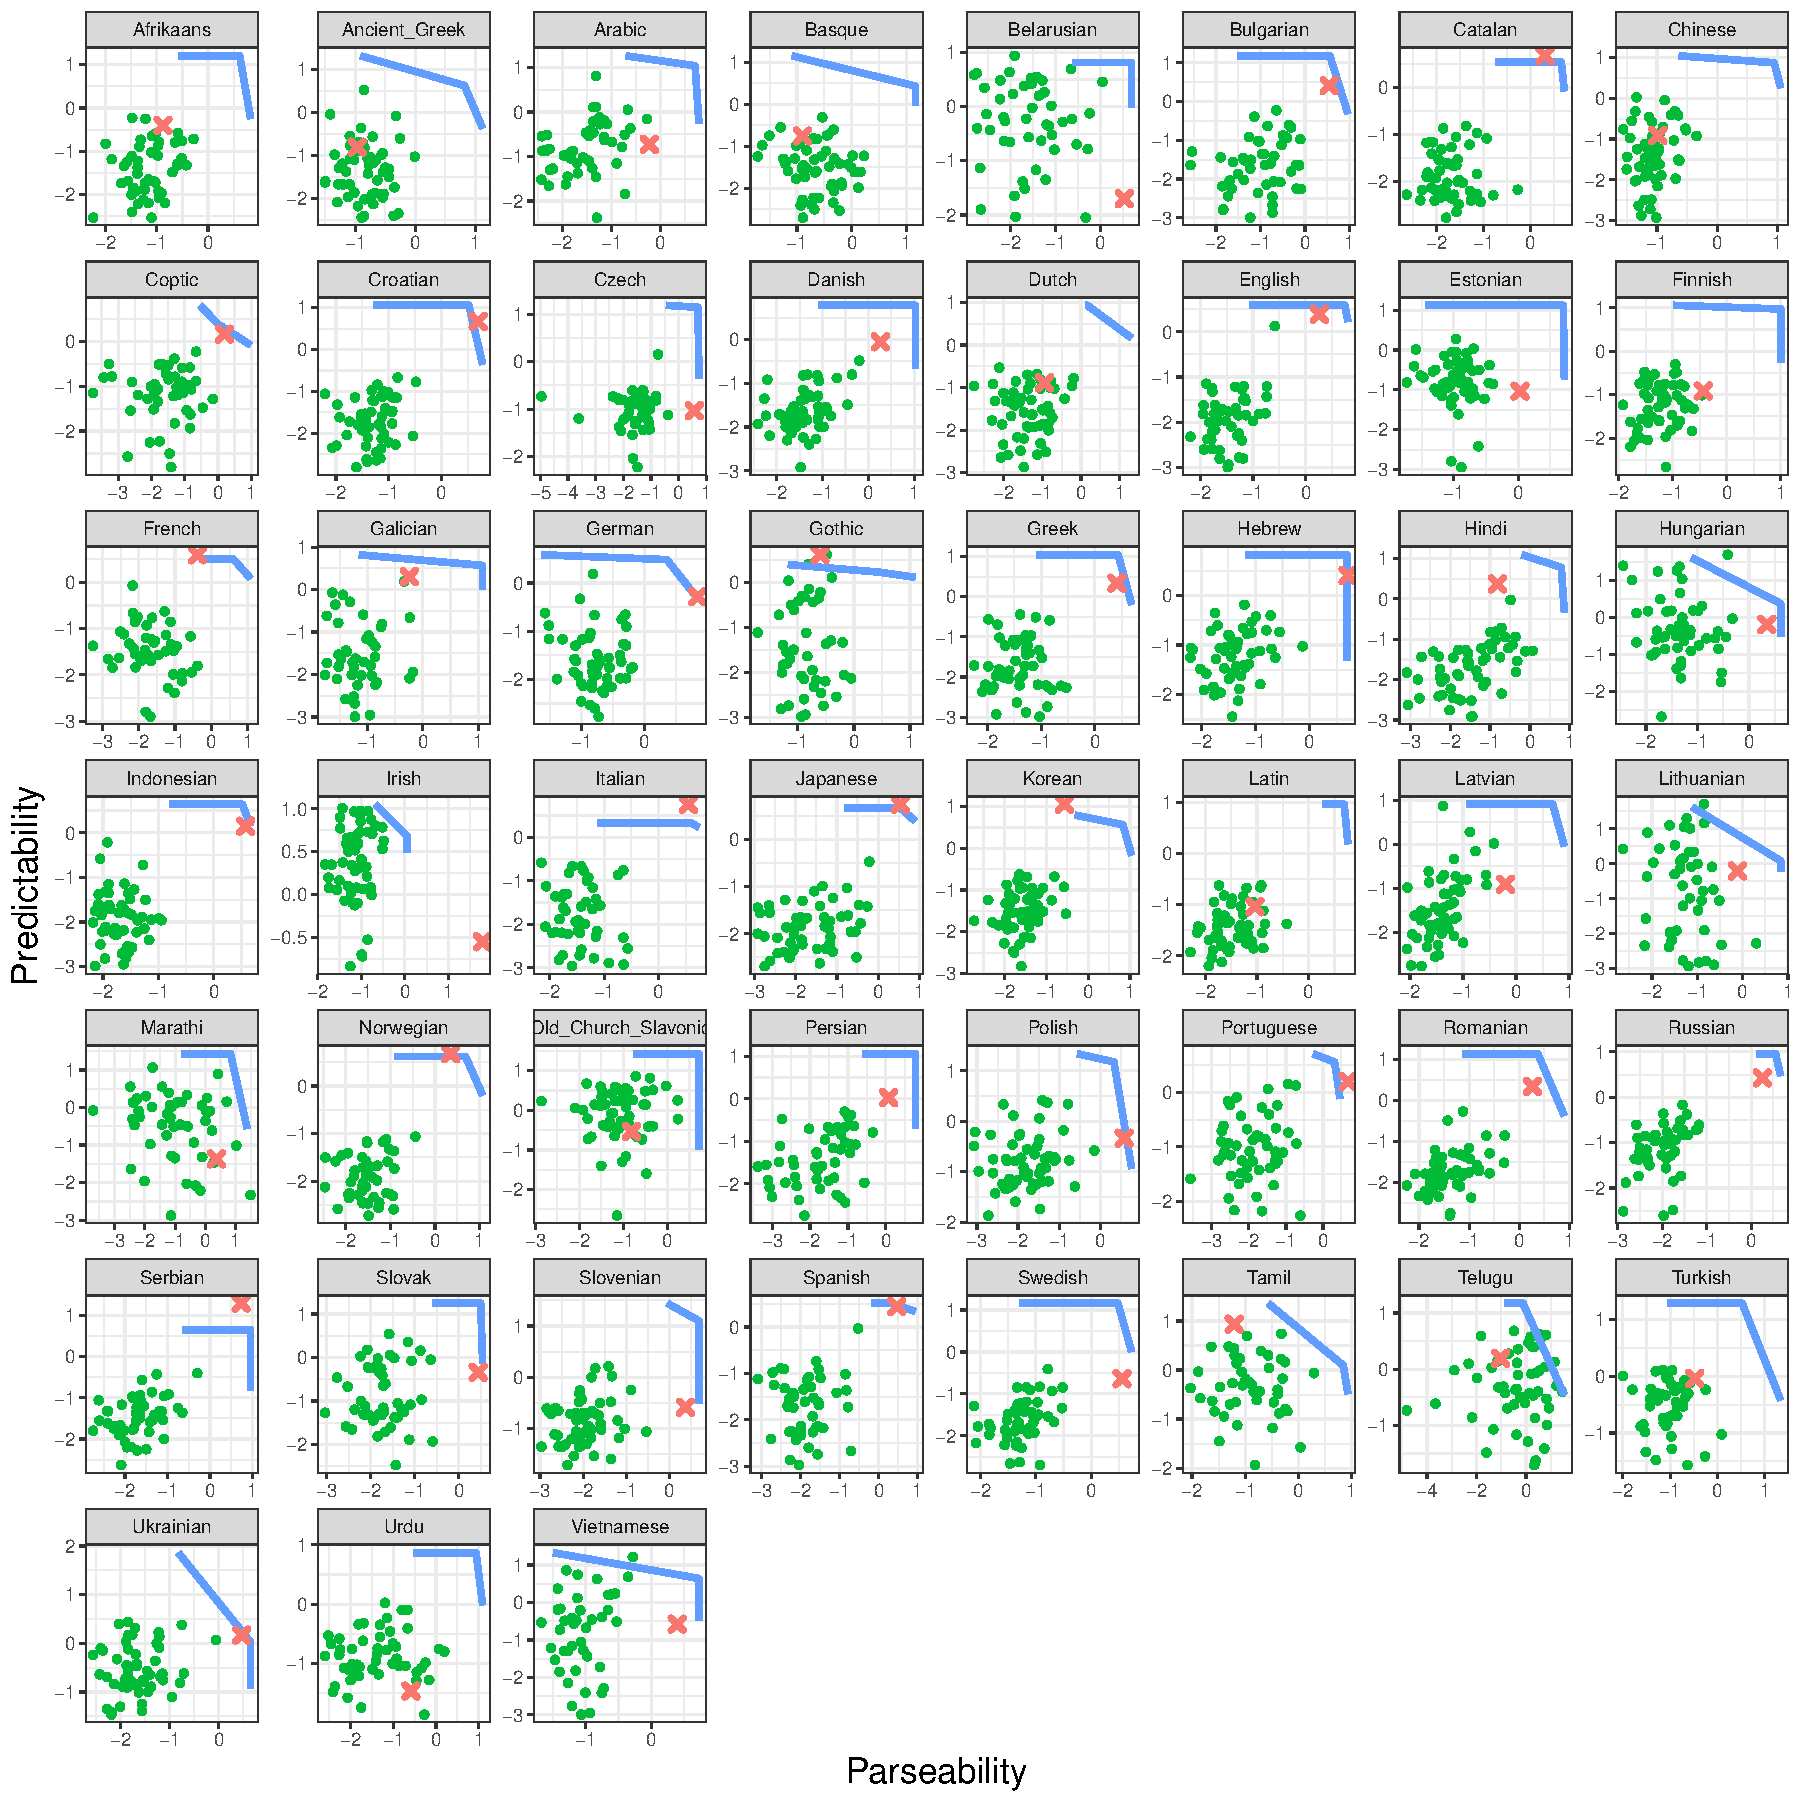
\includegraphics[width=\textwidth]{../results/plane/pareto-plane-perLanguage.pdf}
	\caption[Predictability and Parseability]{Predictability and parseability of 51 languages. Green: random baselines, Red: real grammar, blue: approximate Pareto frontier, computed from the optimized grammars.\footnotemark All data are $z$-scored. Languages are ordered by corpus size, measured by the number of sentences in the training partition, from largest (Czech) to smallest (Irish).}\label{fig:pareto-per-lang}
\end{figure}



\begin{figure}
\centering
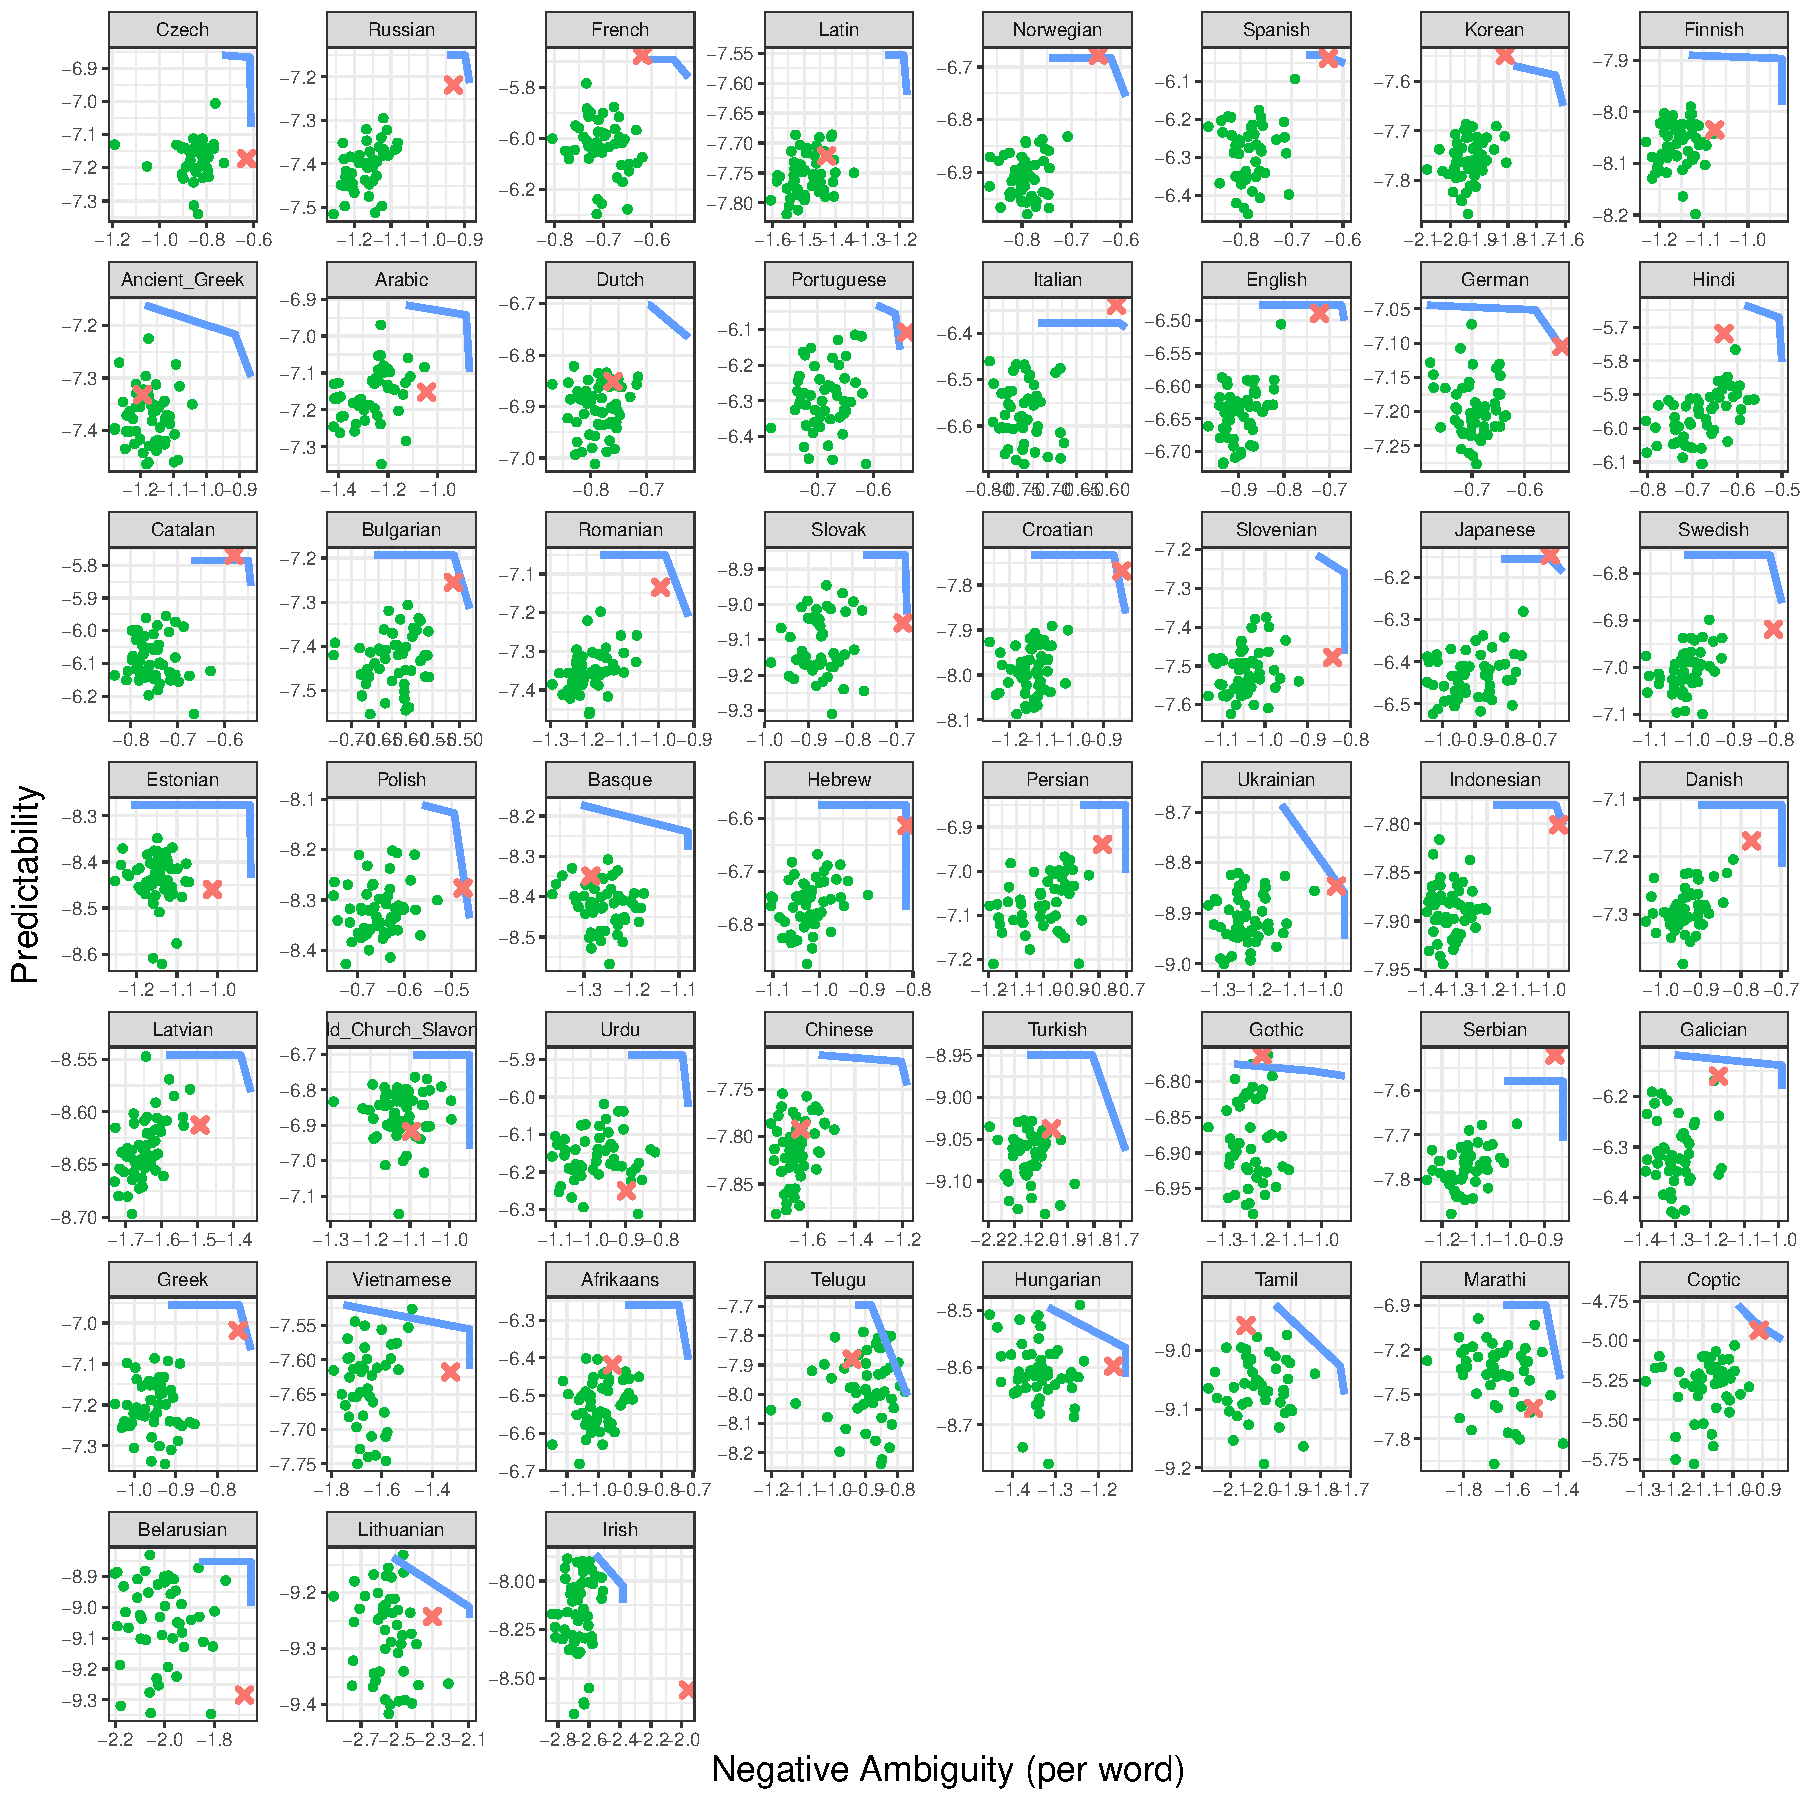
\includegraphics[width=\textwidth]{../results/plane/pareto-plane-perLanguage-raw.pdf}
	\caption[Predictability and Parseability]{Raw numerical values estimated for Predictability (negative surprisal), and negative syntactic ambiguity $-H[T|U]$, before $z$-scoring. For more meaningful comparison, both quantities are normalized by the number of words in the corpus, i.e., we plot per-word negative surprisal and per-word difficulty in recovering syntactic structures.  Note that the negative syntactic ambiguity $-H[T|U]$ equals parseability $I[T,U] = H[T] - H[T|U]$ up to a per-language constant $H[T]$, which we do not attempt to estimate. Further note that we use different scales in the different panels. }\label{fig:pareto-per-lang-raw}
\end{figure}



%\begin{figure}
%\centering
%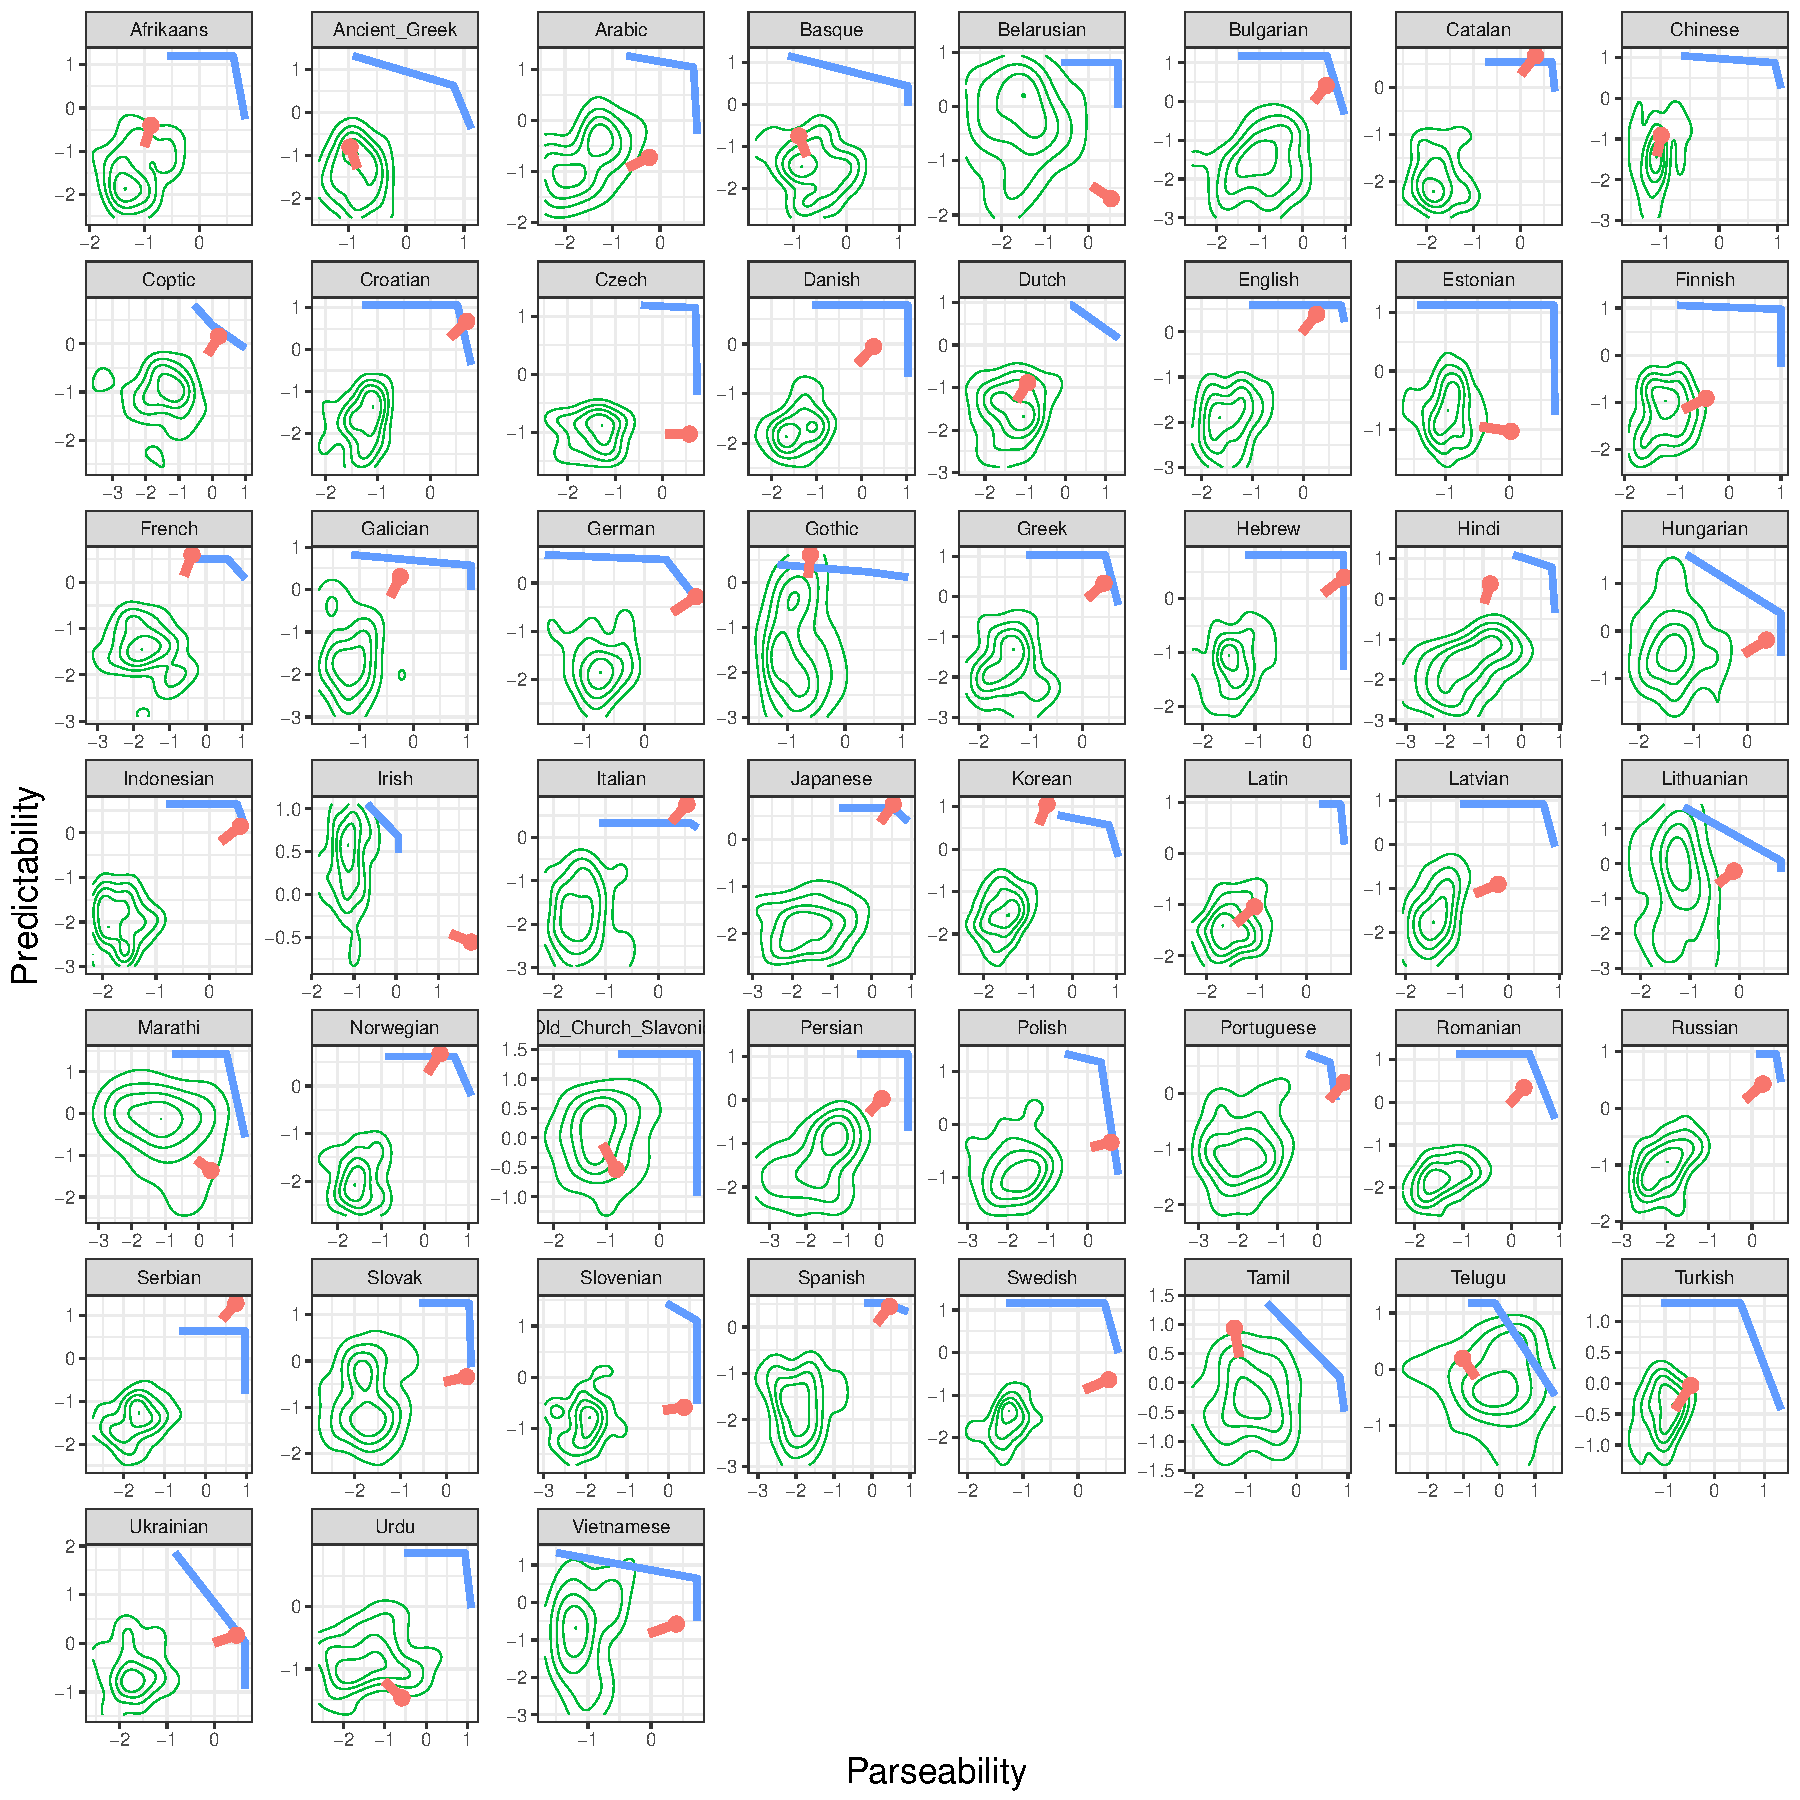
\includegraphics[width=\textwidth]{../results/plane/pareto-plane-perLanguage-arrows-smoothed.pdf}
%\caption[Predictability and Parseability]{Smoothed version with arrows. Is this useful?}\label{fig:pareto-per-lang-arrows}
%\end{figure}
%



\footnotetext{Note that, in a few languages, the real grammar is at a position slightly \emph{beyond} the estimated Pareto frontier. This can be attributed to two reasons: First, stochastic gradient descent introduces noise due to its stochasticity and will only approximately find an optimal solution; second, for some corpora, there may be some degree of distributional mismatch between the training partitions (on which grammars are optimized) and held-out partitions (on which efficiency is estimated). This in particular applies to very small corpora such as Irish (121 training sentences).}


In the main paper, we tested whether real grammars are more efficient than the mean of random grammars, using a $t$-test.
We also conducted the analysis using a Binomial test (one-sided), testing whether the real gramar is more efficient than the \emph{median} of random grammars, avoiding any distributional assumption on the random grammars.
As before, we used Hochberg's step-up procedure (Note that the tests for different languages are independent, as different random grammars are evaluated for each language), with $\alpha=0.05$.
In this analysis, real grammars improved in parseability for 80\% of languages, in predictability for 69\% of languages, and in either of both in 92\% of languages ($p<0.05$, with Bonferroni correction).
In Table~\ref{fig:pareto-per-lang-stats}, we provide per-language results for the $t$-tests and binomial tests.


\begin{table}
\centering
\small{
\begin{tabular}{l||ll|lll|lll}
Language & Pred. (t) & Parse. (t) & \multicolumn{3}{c|}{Pred. (Binomial)} & \multicolumn{3}{c}{Parseab. (Binomial)} \\ 
&  $p$ & $p$ &  Est. &CI & $p$ & Est. & CI & $p$  \\ \hline \hline
Afrikaans  & \num{5.29e-13} & \num{9.35e-06} & $0.96$ & $[0.89,1]$ & \num{1.59e-13} & $0.72$ & $[0.6,1]$ & \num{0.000748}\\ 
Ancient Greek  & \num{1.17e-07} & \num{1} & $0.8$ & $[0.69,1]$ & \num{7.01e-06} & $0.29$ & $[0.19,1]$ & \num{0.999}\\ 
Arabic  & \num{0.0774} & \num{<2e-16} & $0.57$ & $[0.44,1]$ & \num{0.196} & $0.96$ & $[0.89,1]$ & \num{4.28e-14}\\ 
Basque  & \num{2.69e-13} & \num{1} & $0.89$ & $[0.79,1]$ & \num{2.9e-09} & $0.24$ & $[0.15,1]$ & \num{1}\\ 
Belarusian  & \num{1} & \num{<2e-16} & $0.14$ & $[0.07,1]$ & \num{1} & $1$ & $[0.95,1]$ & \num{<2e-16}\\ 
Bulgarian  & \num{<2e-16} & \num{<2e-16} & $1$ & $[0.94,1]$ & \num{8.88e-16} & $1$ & $[0.95,1]$ & \num{<2e-16}\\ 
Catalan  & \num{<2e-16} & \num{<2e-16} & $1$ & $[0.95,1]$ & \num{<2e-16} & $1$ & $[0.95,1]$ & \num{<2e-16}\\ 
Chinese  & \num{1.56e-06} & \num{0.00084} & $0.75$ & $[0.64,1]$ & \num{0.000117} & $0.73$ & $[0.62,1]$ & \num{0.000343}\\ 
Coptic  & \num{0.00175} & \num{<2e-16} & $1$ & $[0.94,1]$ & \num{1.78e-15} & $1$ & $[0.95,1]$ & \num{<2e-16}\\ 
Croatian  & \num{<2e-16} & \num{<2e-16} & $1$ & $[0.94,1]$ & \num{4.44e-16} & $1$ & $[0.95,1]$ & \num{<2e-16}\\ 
Czech  & \num{0.438} & \num{<2e-16} & $0.46$ & $[0.34,1]$ & \num{0.756} & $1$ & $[0.94,1]$ & \num{4.44e-16}\\ 
Danish  & \num{<2e-16} & \num{<2e-16} & $1$ & $[0.95,1]$ & \num{<2e-16} & $1$ & $[0.95,1]$ & \num{<2e-16}\\ 
Dutch  & \num{1.41e-11} & \num{1} & $0.87$ & $[0.77,1]$ & \num{6.54e-09} & $0.27$ & $[0.18,1]$ & \num{1}\\ 
English  & \num{<2e-16} & \num{<2e-16} & $1$ & $[0.94,1]$ & \num{1.78e-15} & $1$ & $[0.95,1]$ & \num{<2e-16}\\ 
Estonian  & \num{0.942} & \num{<2e-16} & $0.27$ & $[0.18,1]$ & \num{1} & $1$ & $[0.95,1]$ & \num{<2e-16}\\ 
Finnish  & \num{8.85e-06} & \num{<2e-16} & $0.7$ & $[0.58,1]$ & \num{0.00274} & $1$ & $[0.95,1]$ & \num{<2e-16}\\ 
French  & \num{4.22e-09} & \num{<2e-16} & $1$ & $[0.94,1]$ & \num{8.88e-16} & $0.98$ & $[0.91,1]$ & \num{1.18e-14}\\ 
Galician  & \num{8.48e-15} & \num{<2e-16} & $1$ & $[0.94,1]$ & \num{1.78e-15} & $0.95$ & $[0.87,1]$ & \num{4.07e-13}\\ 
German  & \num{<2e-16} & \num{<2e-16} & $0.98$ & $[0.91,1]$ & \num{1.18e-14} & $1$ & $[0.95,1]$ & \num{<2e-16}\\ 
Gothic  & \num{9.98e-16} & \num{0.64} & $0.98$ & $[0.91,1]$ & \num{6e-15} & $0.48$ & $[0.36,1]$ & \num{0.658}\\ 
Greek  & \num{<2e-16} & \num{<2e-16} & $1$ & $[0.95,1]$ & \num{<2e-16} & $1$ & $[0.95,1]$ & \num{<2e-16}\\ 
Hebrew  & \num{<2e-16} & \num{<2e-16} & $1$ & $[0.95,1]$ & \num{<2e-16} & $1$ & $[0.95,1]$ & \num{<2e-16}\\ 
Hindi  & \num{<2e-16} & \num{1.41e-10} & $1$ & $[0.95,1]$ & \num{<2e-16} & $0.87$ & $[0.77,1]$ & \num{2e-08}\\ 
Hungarian  & \num{0.127} & \num{<2e-16} & $0.66$ & $[0.54,1]$ & \num{0.0135} & $1$ & $[0.95,1]$ & \num{<2e-16}\\ 
Indonesian  & \num{<2e-16} & \num{<2e-16} & $1$ & $[0.95,1]$ & \num{<2e-16} & $1$ & $[0.95,1]$ & \num{<2e-16}\\ 
Irish  & \num{0.982} & \num{<2e-16} & $0.09$ & $[0.04,1]$ & \num{1} & $1$ & $[0.96,1]$ & \num{<2e-16}\\ 
Italian  & \num{<2e-16} & \num{<2e-16} & $1$ & $[0.94,1]$ & \num{4.44e-16} & $1$ & $[0.94,1]$ & \num{4.44e-16}\\ 
Japanese  & \num{<2e-16} & \num{<2e-16} & $1$ & $[0.95,1]$ & \num{<2e-16} & $1$ & $[0.95,1]$ & \num{<2e-16}\\ 
Korean  & \num{<2e-16} & \num{<2e-16} & $1$ & $[0.95,1]$ & \num{<2e-16} & $0.98$ & $[0.92,1]$ & \num{1.55e-15}\\ 
Latin  & \num{3.97e-09} & \num{2.37e-07} & $0.79$ & $[0.67,1]$ & \num{1.79e-05} & $0.8$ & $[0.69,1]$ & \num{7.01e-06}\\ 
Latvian  & \num{1.14e-06} & \num{<2e-16} & $0.76$ & $[0.65,1]$ & \num{5.68e-05} & $1$ & $[0.95,1]$ & \num{<2e-16}\\ 
Lithuanian  & \num{0.000234} & \num{<2e-16} & $0.62$ & $[0.5,1]$ & \num{0.0492} & $0.98$ & $[0.91,1]$ & \num{6e-15}\\ 
Marathi  & \num{1} & \num{<2e-16} & $0.18$ & $[0.1,1]$ & \num{1} & $1$ & $[0.95,1]$ & \num{<2e-16}\\ 
Norwegian  & \num{<2e-16} & \num{<2e-16} & $1$ & $[0.94,1]$ & \num{1.42e-14} & $1$ & $[0.94,1]$ & \num{2.22e-16}\\ 
Old Church Slavonic  & \num{1} & \num{1.6e-05} & $0.19$ & $[0.1,1]$ & \num{1} & $0.73$ & $[0.62,1]$ & \num{0.000343}\\ 
Persian  & \num{<2e-16} & \num{<2e-16} & $1$ & $[0.94,1]$ & \num{2.22e-16} & $1$ & $[0.95,1]$ & \num{<2e-16}\\ 
Polish  & \num{3.57e-08} & \num{<2e-16} & $0.8$ & $[0.69,1]$ & \num{4.35e-06} & $1$ & $[0.95,1]$ & \num{<2e-16}\\ 
Portuguese  & \num{0.00814} & \num{<2e-16} & $1$ & $[0.95,1]$ & \num{<2e-16} & $1$ & $[0.95,1]$ & \num{<2e-16}\\ 
Romanian  & \num{<2e-16} & \num{<2e-16} & $1$ & $[0.95,1]$ & \num{<2e-16} & $1$ & $[0.95,1]$ & \num{<2e-16}\\ 
Russian  & \num{<2e-16} & \num{<2e-16} & $1$ & $[0.94,1]$ & \num{4.44e-16} & $1$ & $[0.95,1]$ & \num{<2e-16}\\ 
Serbian  & \num{<2e-16} & \num{<2e-16} & $1$ & $[0.94,1]$ & \num{2.22e-16} & $1$ & $[0.95,1]$ & \num{<2e-16}\\ 
Slovak  & \num{6.14e-06} & \num{<2e-16} & $0.67$ & $[0.54,1]$ & \num{0.0129} & $1$ & $[0.95,1]$ & \num{<2e-16}\\ 
Slovenian  & \num{1.79e-05} & \num{<2e-16} & $0.8$ & $[0.69,1]$ & \num{7.01e-06} & $1$ & $[0.95,1]$ & \num{<2e-16}\\ 
Spanish  & \num{5.09e-13} & \num{<2e-16} & $1$ & $[0.94,1]$ & \num{8.88e-16} & $1$ & $[0.95,1]$ & \num{<2e-16}\\ 
Swedish  & \num{<2e-16} & \num{<2e-16} & $0.98$ & $[0.91,1]$ & \num{6e-15} & $1$ & $[0.95,1]$ & \num{<2e-16}\\ 
Tamil  & \num{5.43e-13} & \num{<2e-16} & $1$ & $[0.94,1]$ & \num{1.78e-15} & $0.94$ & $[0.86,1]$ & \num{1.46e-12}\\ 
Telugu  & \num{8.2e-07} & \num{0.00797} & $0.8$ & $[0.69,1]$ & \num{7.01e-06} & $0.59$ & $[0.47,1]$ & \num{0.11}\\ 
Turkish  & \num{6.95e-07} & \num{5.06e-16} & $0.88$ & $[0.78,1]$ & \num{1.62e-08} & $0.92$ & $[0.84,1]$ & \num{3.53e-11}\\ 
Ukrainian  & \num{5.79e-15} & \num{<2e-16} & $0.87$ & $[0.77,1]$ & \num{6.54e-09} & $1$ & $[0.95,1]$ & \num{<2e-16}\\ 
Urdu  & \num{1} & \num{4.84e-11} & $0.1$ & $[0.04,1]$ & \num{1} & $0.83$ & $[0.72,1]$ & \num{1.02e-06}\\ 
Vietnamese  & \num{0.00274} & \num{<2e-16} & $0.54$ & $[0.41,1]$ & \num{0.333} & $1$ & $[0.95,1]$ & \num{<2e-16}\\ 

\end{tabular}
}
\caption{Per-language results in Study 1. For each language, we show the following: (1) $p$-values obtained from a one-sided $t$-test, for the null that the mean predictability/parseability of random grammars is at least as high as that of the real grammar. (2) Results from one-sided binomial tests, for the null that the the real grammar is better than at most $50 \%$ of random grammars. In addition to the $p$-value, we report point estimate and 95\% confidence interval for the fraction of random grammars that have values below real grammars.}\label{fig:pareto-per-lang-stats}
\end{table}

%
%
%\begin{table}
%\centering
%\small{
%\begin{tabular}{l||ll|lll|lll}
%Language & Pred. (t) & Parse. (t) & \multicolumn{3}{c|}{Pred. (Binomial)} & \multicolumn{3}{c}{Parseab. (Binomial)} \\ 
%&  $p$ & $p$ &  Est. &CI & $p$ & Est. & CI & $p$  \\ \hline \hline
%Afrikaans  & \num{5.29e-13} & \num{9.35e-06} & $0.96$ & $[0.89,1]$ & \num{1.59e-13} & $0.72$ & $[0.6,1]$ & \num{0.000748}\\ 
Ancient Greek  & \num{1.17e-07} & \num{1} & $0.8$ & $[0.69,1]$ & \num{7.01e-06} & $0.29$ & $[0.19,1]$ & \num{0.999}\\ 
Arabic  & \num{0.0774} & \num{<2e-16} & $0.57$ & $[0.44,1]$ & \num{0.196} & $0.96$ & $[0.89,1]$ & \num{4.28e-14}\\ 
Basque  & \num{2.69e-13} & \num{1} & $0.89$ & $[0.79,1]$ & \num{2.9e-09} & $0.24$ & $[0.15,1]$ & \num{1}\\ 
Belarusian  & \num{1} & \num{<2e-16} & $0.14$ & $[0.07,1]$ & \num{1} & $1$ & $[0.95,1]$ & \num{<2e-16}\\ 
Bulgarian  & \num{<2e-16} & \num{<2e-16} & $1$ & $[0.94,1]$ & \num{8.88e-16} & $1$ & $[0.95,1]$ & \num{<2e-16}\\ 
Catalan  & \num{<2e-16} & \num{<2e-16} & $1$ & $[0.95,1]$ & \num{<2e-16} & $1$ & $[0.95,1]$ & \num{<2e-16}\\ 
Chinese  & \num{1.56e-06} & \num{0.00084} & $0.75$ & $[0.64,1]$ & \num{0.000117} & $0.73$ & $[0.62,1]$ & \num{0.000343}\\ 
Coptic  & \num{0.00175} & \num{<2e-16} & $1$ & $[0.94,1]$ & \num{1.78e-15} & $1$ & $[0.95,1]$ & \num{<2e-16}\\ 
Croatian  & \num{<2e-16} & \num{<2e-16} & $1$ & $[0.94,1]$ & \num{4.44e-16} & $1$ & $[0.95,1]$ & \num{<2e-16}\\ 
Czech  & \num{0.438} & \num{<2e-16} & $0.46$ & $[0.34,1]$ & \num{0.756} & $1$ & $[0.94,1]$ & \num{4.44e-16}\\ 
Danish  & \num{<2e-16} & \num{<2e-16} & $1$ & $[0.95,1]$ & \num{<2e-16} & $1$ & $[0.95,1]$ & \num{<2e-16}\\ 
Dutch  & \num{1.41e-11} & \num{1} & $0.87$ & $[0.77,1]$ & \num{6.54e-09} & $0.27$ & $[0.18,1]$ & \num{1}\\ 
English  & \num{<2e-16} & \num{<2e-16} & $1$ & $[0.94,1]$ & \num{1.78e-15} & $1$ & $[0.95,1]$ & \num{<2e-16}\\ 
Estonian  & \num{0.942} & \num{<2e-16} & $0.27$ & $[0.18,1]$ & \num{1} & $1$ & $[0.95,1]$ & \num{<2e-16}\\ 
Finnish  & \num{8.85e-06} & \num{<2e-16} & $0.7$ & $[0.58,1]$ & \num{0.00274} & $1$ & $[0.95,1]$ & \num{<2e-16}\\ 
French  & \num{4.22e-09} & \num{<2e-16} & $1$ & $[0.94,1]$ & \num{8.88e-16} & $0.98$ & $[0.91,1]$ & \num{1.18e-14}\\ 
Galician  & \num{8.48e-15} & \num{<2e-16} & $1$ & $[0.94,1]$ & \num{1.78e-15} & $0.95$ & $[0.87,1]$ & \num{4.07e-13}\\ 
German  & \num{<2e-16} & \num{<2e-16} & $0.98$ & $[0.91,1]$ & \num{1.18e-14} & $1$ & $[0.95,1]$ & \num{<2e-16}\\ 
Gothic  & \num{9.98e-16} & \num{0.64} & $0.98$ & $[0.91,1]$ & \num{6e-15} & $0.48$ & $[0.36,1]$ & \num{0.658}\\ 
Greek  & \num{<2e-16} & \num{<2e-16} & $1$ & $[0.95,1]$ & \num{<2e-16} & $1$ & $[0.95,1]$ & \num{<2e-16}\\ 
Hebrew  & \num{<2e-16} & \num{<2e-16} & $1$ & $[0.95,1]$ & \num{<2e-16} & $1$ & $[0.95,1]$ & \num{<2e-16}\\ 
Hindi  & \num{<2e-16} & \num{1.41e-10} & $1$ & $[0.95,1]$ & \num{<2e-16} & $0.87$ & $[0.77,1]$ & \num{2e-08}\\ 
Hungarian  & \num{0.127} & \num{<2e-16} & $0.66$ & $[0.54,1]$ & \num{0.0135} & $1$ & $[0.95,1]$ & \num{<2e-16}\\ 
Indonesian  & \num{<2e-16} & \num{<2e-16} & $1$ & $[0.95,1]$ & \num{<2e-16} & $1$ & $[0.95,1]$ & \num{<2e-16}\\ 
Irish  & \num{0.982} & \num{<2e-16} & $0.09$ & $[0.04,1]$ & \num{1} & $1$ & $[0.96,1]$ & \num{<2e-16}\\ 
Italian  & \num{<2e-16} & \num{<2e-16} & $1$ & $[0.94,1]$ & \num{4.44e-16} & $1$ & $[0.94,1]$ & \num{4.44e-16}\\ 
Japanese  & \num{<2e-16} & \num{<2e-16} & $1$ & $[0.95,1]$ & \num{<2e-16} & $1$ & $[0.95,1]$ & \num{<2e-16}\\ 
Korean  & \num{<2e-16} & \num{<2e-16} & $1$ & $[0.95,1]$ & \num{<2e-16} & $0.98$ & $[0.92,1]$ & \num{1.55e-15}\\ 
Latin  & \num{3.97e-09} & \num{2.37e-07} & $0.79$ & $[0.67,1]$ & \num{1.79e-05} & $0.8$ & $[0.69,1]$ & \num{7.01e-06}\\ 
Latvian  & \num{1.14e-06} & \num{<2e-16} & $0.76$ & $[0.65,1]$ & \num{5.68e-05} & $1$ & $[0.95,1]$ & \num{<2e-16}\\ 
Lithuanian  & \num{0.000234} & \num{<2e-16} & $0.62$ & $[0.5,1]$ & \num{0.0492} & $0.98$ & $[0.91,1]$ & \num{6e-15}\\ 
Marathi  & \num{1} & \num{<2e-16} & $0.18$ & $[0.1,1]$ & \num{1} & $1$ & $[0.95,1]$ & \num{<2e-16}\\ 
Norwegian  & \num{<2e-16} & \num{<2e-16} & $1$ & $[0.94,1]$ & \num{1.42e-14} & $1$ & $[0.94,1]$ & \num{2.22e-16}\\ 
Old Church Slavonic  & \num{1} & \num{1.6e-05} & $0.19$ & $[0.1,1]$ & \num{1} & $0.73$ & $[0.62,1]$ & \num{0.000343}\\ 
Persian  & \num{<2e-16} & \num{<2e-16} & $1$ & $[0.94,1]$ & \num{2.22e-16} & $1$ & $[0.95,1]$ & \num{<2e-16}\\ 
Polish  & \num{3.57e-08} & \num{<2e-16} & $0.8$ & $[0.69,1]$ & \num{4.35e-06} & $1$ & $[0.95,1]$ & \num{<2e-16}\\ 
Portuguese  & \num{0.00814} & \num{<2e-16} & $1$ & $[0.95,1]$ & \num{<2e-16} & $1$ & $[0.95,1]$ & \num{<2e-16}\\ 
Romanian  & \num{<2e-16} & \num{<2e-16} & $1$ & $[0.95,1]$ & \num{<2e-16} & $1$ & $[0.95,1]$ & \num{<2e-16}\\ 
Russian  & \num{<2e-16} & \num{<2e-16} & $1$ & $[0.94,1]$ & \num{4.44e-16} & $1$ & $[0.95,1]$ & \num{<2e-16}\\ 
Serbian  & \num{<2e-16} & \num{<2e-16} & $1$ & $[0.94,1]$ & \num{2.22e-16} & $1$ & $[0.95,1]$ & \num{<2e-16}\\ 
Slovak  & \num{6.14e-06} & \num{<2e-16} & $0.67$ & $[0.54,1]$ & \num{0.0129} & $1$ & $[0.95,1]$ & \num{<2e-16}\\ 
Slovenian  & \num{1.79e-05} & \num{<2e-16} & $0.8$ & $[0.69,1]$ & \num{7.01e-06} & $1$ & $[0.95,1]$ & \num{<2e-16}\\ 
Spanish  & \num{5.09e-13} & \num{<2e-16} & $1$ & $[0.94,1]$ & \num{8.88e-16} & $1$ & $[0.95,1]$ & \num{<2e-16}\\ 
Swedish  & \num{<2e-16} & \num{<2e-16} & $0.98$ & $[0.91,1]$ & \num{6e-15} & $1$ & $[0.95,1]$ & \num{<2e-16}\\ 
Tamil  & \num{5.43e-13} & \num{<2e-16} & $1$ & $[0.94,1]$ & \num{1.78e-15} & $0.94$ & $[0.86,1]$ & \num{1.46e-12}\\ 
Telugu  & \num{8.2e-07} & \num{0.00797} & $0.8$ & $[0.69,1]$ & \num{7.01e-06} & $0.59$ & $[0.47,1]$ & \num{0.11}\\ 
Turkish  & \num{6.95e-07} & \num{5.06e-16} & $0.88$ & $[0.78,1]$ & \num{1.62e-08} & $0.92$ & $[0.84,1]$ & \num{3.53e-11}\\ 
Ukrainian  & \num{5.79e-15} & \num{<2e-16} & $0.87$ & $[0.77,1]$ & \num{6.54e-09} & $1$ & $[0.95,1]$ & \num{<2e-16}\\ 
Urdu  & \num{1} & \num{4.84e-11} & $0.1$ & $[0.04,1]$ & \num{1} & $0.83$ & $[0.72,1]$ & \num{1.02e-06}\\ 
Vietnamese  & \num{0.00274} & \num{<2e-16} & $0.54$ & $[0.41,1]$ & \num{0.333} & $1$ & $[0.95,1]$ & \num{<2e-16}\\ 

%\end{tabular}
%}
%\caption{Per-language results in Study 1. For each language, we show the following: (1) $p$-values obtained from a one-sided $t$-test, for the null that the mean predictability/parseability of random grammars is at least as high as that of the real grammar. (2) Results from one-sided binomial tests, for the null that the the real grammar is better than at most $50 \%$ of random grammars. In addition to the $p$-value, we report point estimate and 95\% confidence interval for the fraction of random grammars that have values below real grammars.}\label{fig:pareto-per-lang-stats}
%\end{table}
%
%


\subsection{Analysis controlling for Families}

The UD treebanks overrepresent certain language families.
Does this impact the results of Study 1?
We estimate the overall degree of optimization of languages for efficiency, controlling for differences between families, we constructed a Bayesian logistic mixed-effects model estimating, for each language $L$ among the 51 UD languages, the rate $q_L \in [0,1]$ of random baseline grammars that have lower efficiency (parseability, predictability) than the real grammar.
We entered languages and language families as random effects:
\begin{equation}\label{eq:mixed-effects-study1}
logit(q_{L}) = \beta + u_{L} + v_{f_L}
\end{equation}
where $f_L$ is the language family of $L$.

Results for the posterior of $\beta$ are shown in Table~\ref{tab:study1-glmer}.
Across language families, real grammars tend to be more efficient than almost all baseline grammars.
According to this analysis, exceptions among the UD corpora can be attributed to language-specific effects.

TODO also report glmer, posterior plots, transformed probabilities

\begin{table}
\small{
\begin{center}
\begin{tabular}{|l||l|lll|llll|ll|llllll}
\hline
	& Mean $\beta$ & SD & Lower 95\% CrI & Upper 95\% CrI \\
\hline\hline
	Efficiency ($\lambda=0.9$) &	-5.88   &   1.08  &  -8.28  &  -3.97  \\
	Surp & -3.48   &   0.88  &  -5.42  &  -1.85   \\
	Pars & -5.55   &   1.08  &  -7.80  &  -3.67    \\
\hline
\end{tabular}
\end{center}
}
	\caption{Models estimating the log-odds of a random baseline grammar improving over a real grammar in efficiency ($\lambda=0.9$), surprisal, or parseability, with random effects for languages and language families. The strongly negative estimates of $\beta$ confirm that, across languages and language families, real grammars improve over most baselines. TODO}\label{tab:study1-glmer}
\end{table}

\subsection{Quantifying Degree of Optimality}


\begin{figure}
\centering
		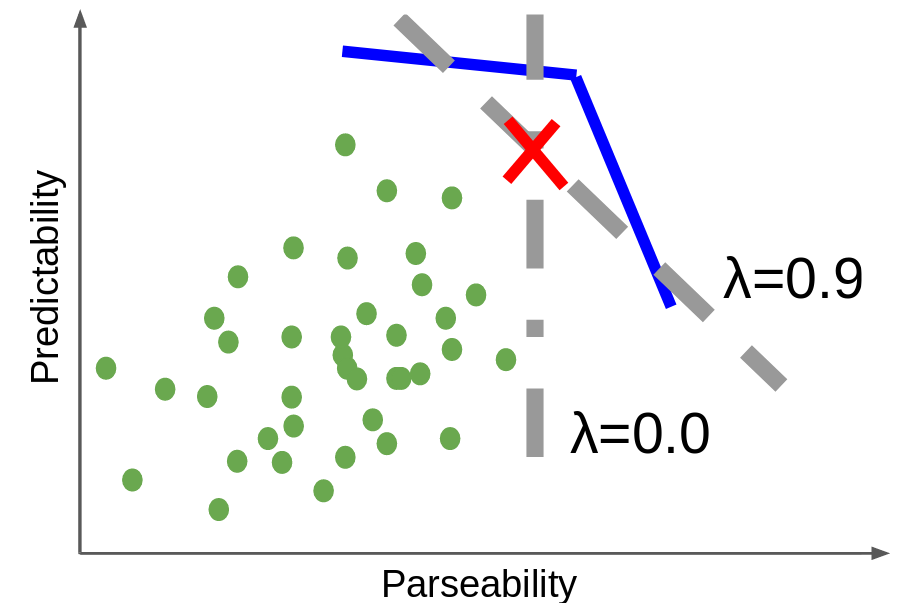
\includegraphics[width=0.5\textwidth]{lambda-explanation.png}

	\caption{For $\lambda=0$ and $\lambda=0.9$, we provide lines connecting points that have the same efficiency value as the real language (red cross). Points to the bottom right of the lines have lower efficiency under the respective values of $\lambda$. In this example, all baseline samples (green dots) have lower efficiency than the real language, even though the real language does not outperform every baselines on both components of efficiency.}\label{fig:opt-lambda-explanation}
\end{figure}


\begin{figure}
\centering
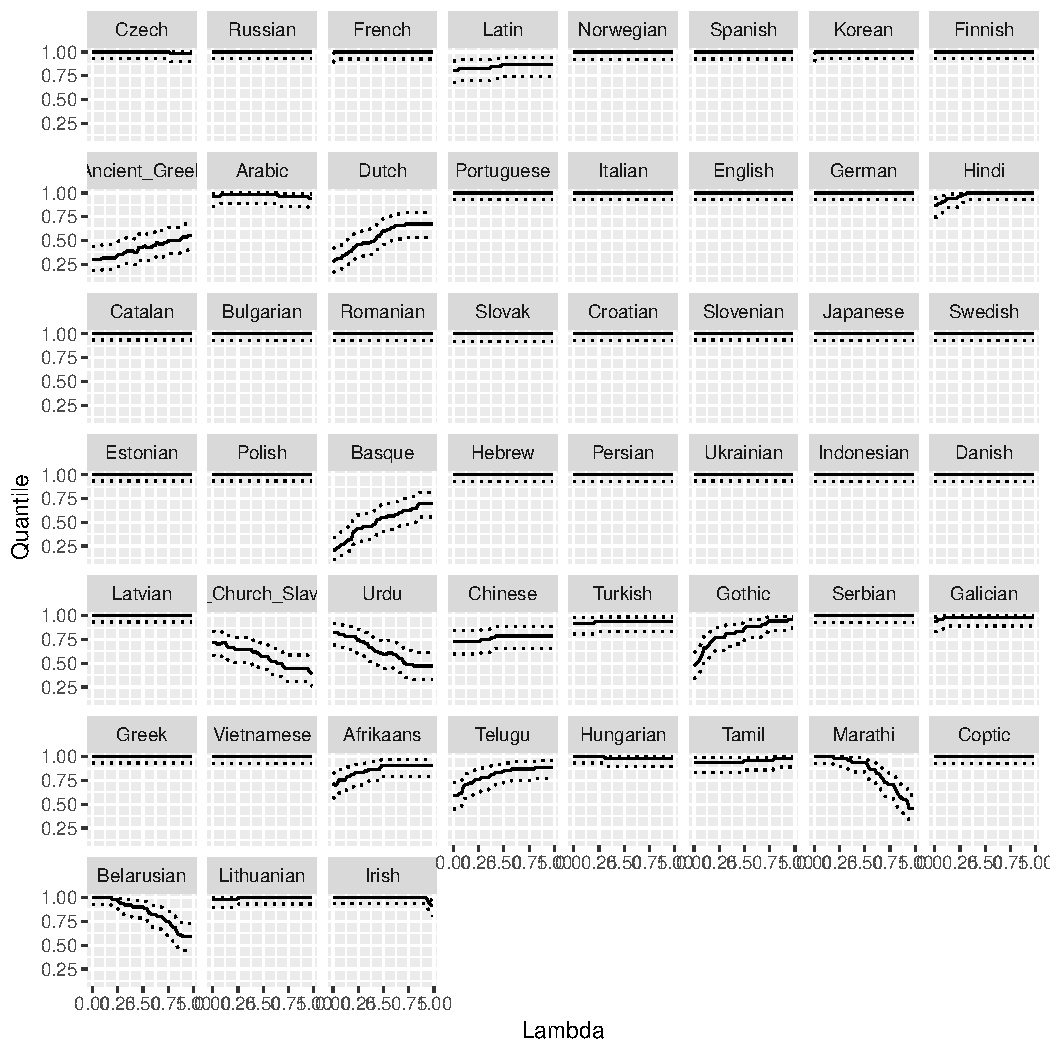
\includegraphics[width=\textwidth]{../results/plane/analyze_pareto_optimality/figures/quantileByLambda.pdf}
	\caption[]{The $x$-axis shows $\lambda \in [0,1)$, the $y$-axis shows the fraction of baselines that have lower efficiency at this value of $\lambda$, with 95\% confidence bands obtained from a binomial test.}\label{fig:lambda-quantile}
\end{figure}

In the main paper (Study 1), we showed that languages tend to be optimized for parseability and/or predictability.
Efficiency is a combination of both components; in this section we address the question whether languages are generally optimized for efficiency, i.e., the multi-objective optimization problem of optimizing for parseability and predictability.
%Note that the numerical value of efficiency depends on the parameter $\lambda \in [0,1)$.

We quantify degree of optimality in two ways.
In Analysis 1, we consider the efficiency metric $R_\lambda := R_{Pars} + \lambda R_{Pred}$ with the tradeoff parameter $\lambda \in [0,1)$.
For each possible value of $\lambda \in [0,1)$ trading off parseability and predictability, we quantify how many baseline grammars are less efficient than the real language.
In Analysis 2, we quantify what fraction of baseline languages \emph{Pareto-dominates} the real language, showing that -- while not all real languages may be strongly optimized for both objectives individually -- at most a very small fraction of baseline grammars improve on the real language on both components.

\paragraph{Analysis 1: Optimality by $\lambda$}
%Second, we quantify how many baseline languages are more efficient across all values of $\lambda$.

Recall the efficiency metric
\begin{equation}
	R_\lambda := R_{Pars} + \lambda R_{Pred}
\end{equation}
 with the tradeoff parameter $\lambda \in [0,1)$.
For each $\lambda$, we quantify the fraction of baselines that have better efficiency than the real language:
\begin{equation}
	O_\lambda := \frac{\# \{b \in B: R_{\lambda}(b) > R_{\lambda}(r)\}}{\# B}
\end{equation}
where $B$ is the set of baseline languages.
We illustrate this in Figure~\ref{fig:opt-lambda-explanation}.

The results are plotted in Figure~\ref{fig:lambda-quantile}.

For all languages, there are some values of $\lambda$ where the real language improves at least on more than the median of the baseline grammars, i.e., $O_\lambda >0$.
In about 40 of the languages, $O_\lambda$ is even close to one across all values of $\lambda$.

This shows that, while many languages do not improve over \emph{all} baselines on \emph{both} individual components, they mostly improve over the large majority of baselines on the combined objective of efficiency, even across different values of $\lambda$.


\begin{figure}
\centering
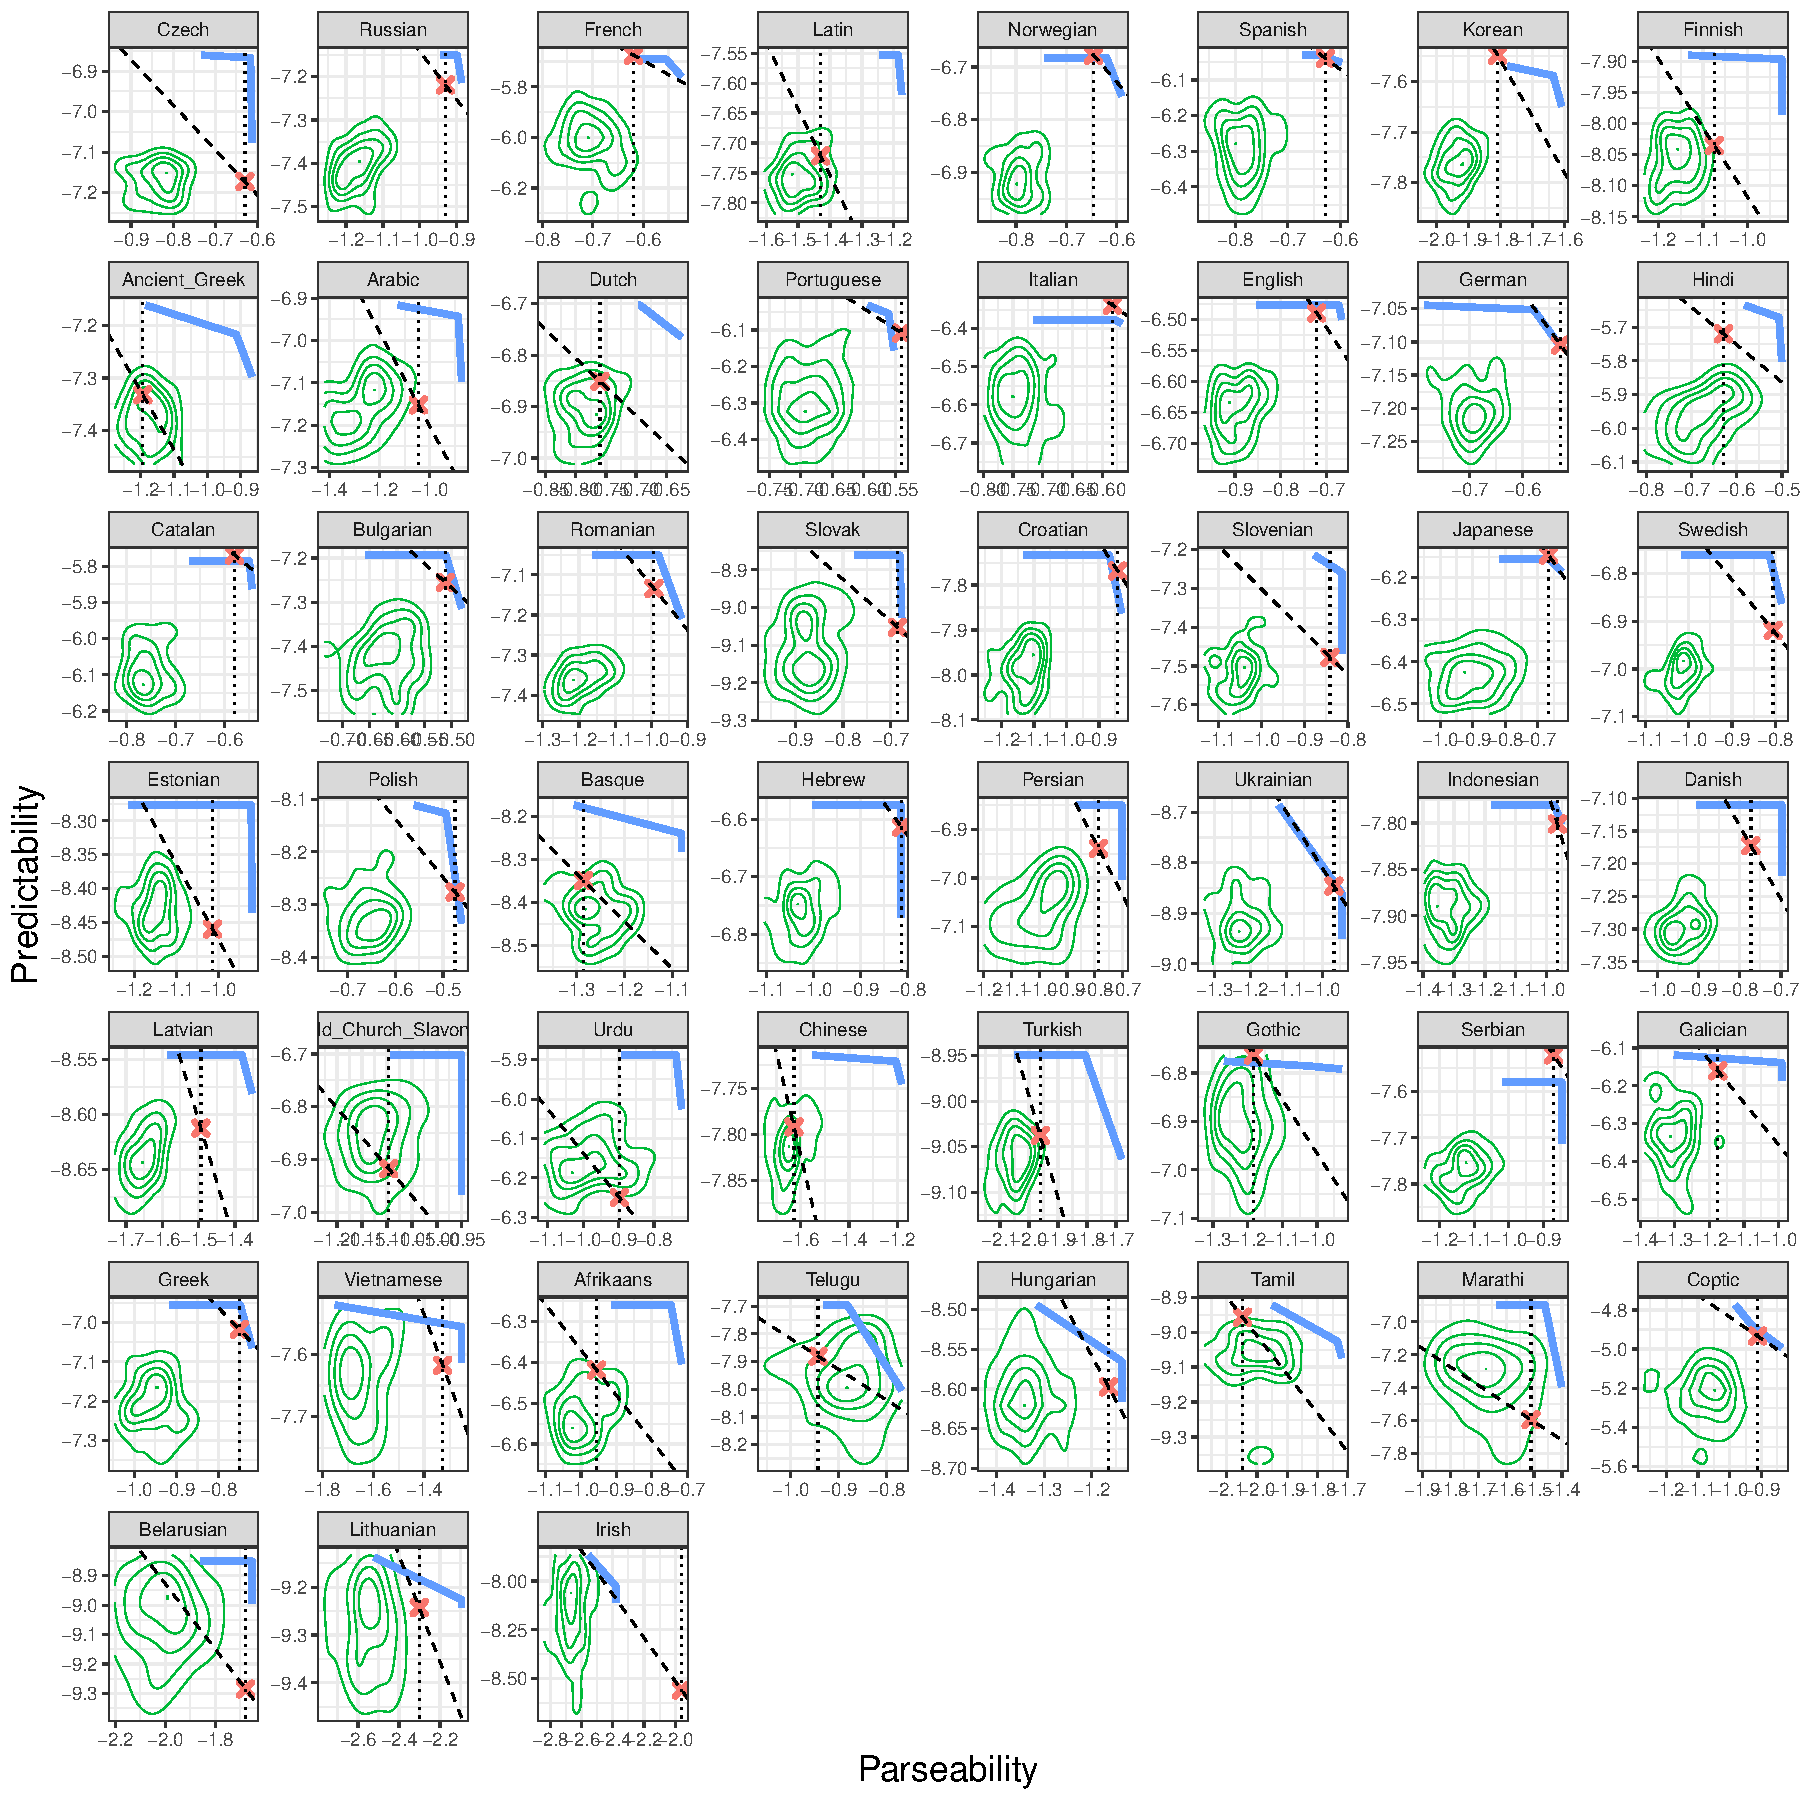
\includegraphics[width=\textwidth]{../results/plane/analyze_pareto_optimality/pareto-plane-perLanguage-arrows-smoothed-halfspace-untransformed.pdf}
	\caption[]{Per-Language results as in Figure~\ref{fig:pareto-per-lang-raw}, with lines connecting those points that have the same efficiency as the real grammar at $\lambda = 0.0$ (dotted) and $\lambda = 0.9$ (dashed). Points to the bottom/left of these line have lower efficiency than the real grammar, at the given value of $\lambda$.}\label{fig:lambda-halfplane-09}
\end{figure}

TODO
We note that not all real grammars are on the estimated Pareto frontier.
TODO discuss difference from semantic typology:
TODO mention that, in semantic typology, random baselines might tend to be closer to the frontier, whereas, in our study, there tends to be a low-density region between the baseline grammars and the optimum (as also observed in previous DLM and surprisal studies, cite Futrell and Gildea/Jaeger). 




\subsection{Parseability and Surprisal Metrics for Observed Orders and Extracted Grammars}

In Table~\ref{tab:observed-and-extracted}, we report parsing and surprisal metrics that are commonly used in the NLP literature, both for the originally observed orders in the corpora, and the corpora ordered according to the real grammars as extracted and expressed in our grammar formalism.
We observe similar performance on observed orders and the extracted grammars, across all metrics.
We note that, while our parsing model is based on the strongest available dependency parsing method from the NLP literature \cite{dozat2017stanford,zeman2018proceedings,che2018towards}, the parsing metrics here are mostly below the best numbers reported with this architecture \cite{zeman2018proceedings} due to the use of an unlexicalized parsing model.


\begin{table}
\centering
\small{
\begin{tabular}{l||ll|ll|l||ll|ll|l|lllll}
	Language & \multicolumn{5}{c||}{Observed Orders} & \multicolumn{5}{c|}{Extracted Grammars} \\ 
	& UAS & LAS & U.Pars. & L.Pars. & Surp. & UAS & LAS & U.Pars. & L.Pars. & Surp.\\ \hline \hline
Afrikaans  &  0.798  &  0.757  &  0.754  &  1.005  &  6.341  &  0.799  &  0.763  &  0.738  &  0.951  &  6.419  &  \\ 
Ancient Greek  &  0.634  &  0.539  &  1.141  &  1.716  &  7.345  &  0.748  &  0.66  &  0.801  &  1.196  &  7.332  &  \\ 
Arabic  &  0.785  &  0.726  &  0.73  &  1.036  &  6.872  &  0.77  &  0.709  &  0.759  &  1.06  &  7.152  &  \\ 
Basque  &  0.714  &  0.562  &  0.879  &  1.512  &  8.344  &  0.736  &  0.624  &  0.858  &  1.293  &  8.349  &  \\ 
Belarusian  &  0.684  &  0.606  &  1.263  &  1.865  &  9.127  &  0.675  &  0.615  &  1.21  &  1.73  &  9.285  &  \\ 
Bulgarian  &  0.883  &  0.815  &  0.378  &  0.62  &  7.15  &  0.894  &  0.846  &  0.336  &  0.497  &  7.255  &  \\ 
Catalan  &  0.864  &  0.806  &  0.457  &  0.681  &  5.691  &  0.873  &  0.838  &  0.447  &  0.586  &  5.769  &  \\ 
Chinese  &  0.593  &  0.554  &  1.301  &  1.68  &  7.682  &  0.594  &  0.547  &  1.234  &  1.617  &  7.792  &  \\ 
Coptic  &  0.829  &  0.749  &  0.634  &  1.041  &  4.869  &  0.84  &  0.772  &  0.597  &  0.891  &  4.933  &  \\ 
Croatian  &  0.796  &  0.725  &  0.696  &  1.081  &  7.766  &  0.816  &  0.771  &  0.611  &  0.869  &  7.769  &  \\ 
Czech  &  0.824  &  0.763  &  0.558  &  0.858  &  7.156  &  0.853  &  0.813  &  0.519  &  0.63  &  7.173  &  \\ 
Danish  &  0.801  &  0.75  &  0.73  &  1.017  &  7.043  &  0.841  &  0.802  &  0.55  &  0.764  &  7.173  &  \\ 
Dutch  &  0.839  &  0.782  &  0.573  &  0.897  &  6.826  &  0.835  &  0.792  &  0.57  &  0.808  &  6.851  &  \\ 
English  &  0.834  &  0.788  &  0.552  &  0.837  &  6.396  &  0.843  &  0.806  &  0.498  &  0.728  &  6.489  &  \\ 
Estonian  &  0.742  &  0.602  &  0.814  &  1.344  &  8.371  &  0.784  &  0.709  &  0.681  &  0.997  &  8.46  &  \\ 
Finnish  &  0.728  &  0.616  &  0.814  &  1.306  &  7.959  &  0.754  &  0.686  &  0.755  &  1.07  &  8.035  &  \\ 
French  &  0.856  &  0.8  &  0.493  &  0.752  &  5.72  &  0.873  &  0.832  &  0.425  &  0.617  &  5.675  &  \\ 
Galician  &  0.777  &  0.718  &  0.77  &  1.213  &  6.12  &  0.774  &  0.718  &  0.784  &  1.175  &  6.16  &  \\ 
German  &  0.832  &  0.777  &  0.53  &  0.84  &  7.09  &  0.896  &  0.859  &  0.337  &  0.523  &  7.105  &  \\ 
Gothic  &  0.72  &  0.596  &  0.869  &  1.424  &  7.038  &  0.755  &  0.641  &  0.781  &  1.217  &  6.763  &  \\ 
Greek  &  0.829  &  0.773  &  0.609  &  0.89  &  7.1  &  0.834  &  0.804  &  0.577  &  0.765  &  7.018  &  \\ 
Hebrew  &  0.829  &  0.759  &  0.588  &  0.944  &  6.61  &  0.835  &  0.776  &  0.545  &  0.836  &  6.614  &  \\ 
Hindi  &  0.867  &  0.791  &  0.38  &  0.642  &  5.599  &  0.861  &  0.803  &  0.486  &  0.614  &  5.72  &  \\ 
Hungarian  &  0.741  &  0.622  &  0.909  &  1.419  &  8.572  &  0.758  &  0.678  &  0.855  &  1.18  &  8.597  &  \\ 
Indonesian  &  0.8  &  0.749  &  0.685  &  1.062  &  7.735  &  0.818  &  0.767  &  0.616  &  0.969  &  7.801  &  \\ 
Irish  &  0.659  &  0.542  &  1.244  &  2.122  &  7.772  &  0.721  &  0.598  &  1.023  &  1.84  &  8.558  &  \\ 
Italian  &  0.858  &  0.802  &  0.471  &  0.736  &  6.342  &  0.879  &  0.839  &  0.391  &  0.588  &  6.338  &  \\ 
Japanese  &  0.872  &  0.766  &  0.389  &  0.726  &  6.092  &  0.877  &  0.782  &  0.385  &  0.696  &  6.146  &  \\ 
Korean  &  0.623  &  0.438  &  1.09  &  1.898  &  7.476  &  0.632  &  0.459  &  1.077  &  1.804  &  7.548  &  \\ 
Latin  &  0.606  &  0.492  &  1.238  &  2.005  &  7.735  &  0.733  &  0.621  &  0.873  &  1.446  &  7.722  &  \\ 
Latvian  &  0.65  &  0.53  &  1.121  &  1.767  &  8.629  &  0.658  &  0.597  &  1.07  &  1.493  &  8.612  &  \\ 
Lithuanian  &  0.522  &  0.418  &  1.614  &  2.576  &  9.725  &  0.546  &  0.479  &  1.562  &  2.295  &  9.243  &  \\ 
Marathi  &  0.719  &  0.57  &  1.006  &  1.809  &  7.203  &  0.76  &  0.631  &  0.896  &  1.42  &  7.594  &  \\ 
Norwegian  &  0.859  &  0.801  &  0.447  &  0.761  &  6.678  &  0.879  &  0.829  &  0.378  &  0.653  &  6.678  &  \\ 
Old Church Slavonic  &  0.748  &  0.619  &  0.79  &  1.342  &  7.304  &  0.794  &  0.676  &  0.672  &  1.089  &  6.917  &  \\ 
Persian  &  0.814  &  0.755  &  0.632  &  0.869  &  6.908  &  0.828  &  0.78  &  0.587  &  0.803  &  6.939  &  \\ 
Polish  &  0.852  &  0.782  &  0.461  &  0.725  &  8.389  &  0.91  &  0.858  &  0.357  &  0.481  &  8.276  &  \\ 
Portuguese  &  0.869  &  0.817  &  0.443  &  0.676  &  6.049  &  0.891  &  0.847  &  0.346  &  0.536  &  6.109  &  \\ 
Romanian  &  0.806  &  0.712  &  0.671  &  1.123  &  7.074  &  0.813  &  0.737  &  0.619  &  0.977  &  7.134  &  \\ 
Russian  &  0.782  &  0.696  &  0.706  &  1.146  &  7.155  &  0.809  &  0.742  &  0.607  &  0.923  &  7.219  &  \\ 
Serbian  &  0.825  &  0.757  &  0.617  &  0.992  &  7.556  &  0.832  &  0.766  &  0.576  &  0.894  &  7.521  &  \\ 
Slovak  &  0.831  &  0.772  &  0.543  &  0.849  &  9.199  &  0.849  &  0.817  &  0.495  &  0.696  &  9.053  &  \\ 
Slovenian  &  0.798  &  0.713  &  0.705  &  1.112  &  7.498  &  0.841  &  0.788  &  0.595  &  0.836  &  7.478  &  \\ 
Spanish  &  0.855  &  0.789  &  0.484  &  0.777  &  6.246  &  0.869  &  0.825  &  0.429  &  0.637  &  6.039  &  \\ 
Swedish  &  0.823  &  0.752  &  0.606  &  0.979  &  6.839  &  0.849  &  0.796  &  0.519  &  0.808  &  6.919  &  \\ 
Tamil  &  0.658  &  0.572  &  1.245  &  1.896  &  9  &  0.663  &  0.565  &  1.438  &  1.857  &  8.957  &  \\ 
Telugu  &  0.882  &  0.651  &  0.359  &  1.081  &  7.9  &  0.888  &  0.715  &  0.481  &  0.882  &  7.88  &  \\ 
Turkish  &  0.58  &  0.423  &  1.376  &  2.119  &  8.966  &  0.572  &  0.448  &  1.358  &  1.959  &  9.038  &  \\ 
Ukrainian  &  0.789  &  0.716  &  0.714  &  1.101  &  8.826  &  0.799  &  0.753  &  0.673  &  0.953  &  8.846  &  \\ 
Urdu  &  0.816  &  0.736  &  0.617  &  0.984  &  5.771  &  0.822  &  0.756  &  0.58  &  0.893  &  6.25  &  \\ 
Vietnamese  &  0.627  &  0.583  &  1.142  &  1.601  &  7.536  &  0.696  &  0.653  &  0.986  &  1.345  &  7.618  &  \\ 

\end{tabular}
}
	\caption{Parsing and Surprisal metrics for observed orders (left), and for corpora ordered according to extracted real grammars (right). UAS and LAS refer to \emph{Unlabeled} and \emph{Labeled Attachment Scores}, respectively, indicating what fraction of words is assigned the correct head (UAS) or the correct head and relation label (LAS) when choosing heads and labels assigned the highest probability $p_\phi(\text{head}_i, \text{label}_i | u, i)$ (Equation~\ref{eq:pars-obj}) by the parser.
	U.Pars refers to the average value of $- \log p_\phi(\text{head}_i| u, i)$, which is a measure of the difficulty of recovering the raw tree structure, without relation labels. 
	L.Pars refers to the average value of $- \log p_\phi(\text{head}_i, \text{label}_i| u, i)$, measuring the difficulty of recoovering tree structures including relation labels.
	Note that L.Pars corresponds to $\operatorname{H}[\tree|\utterance]$ normalized by the number of words.
	Finally, Surp. refers to the average word-by-word surprisal, which corresponds to the predictability measure $\operatorname{H}[\utterance]$ normalized by the number of words.
	}\label{tab:observed-and-extracted}
\end{table}




\section{Supplementary Analyses for Study 2}
\subsection{Correlation between Universals and Efficiency}

In Figure~\ref{fig:corr-eff-corr}, we plot efficiency, parseability, and predictability (all are $z$-scored within language, as in Study 1) as a function of the number of satisfied correlations, for the real grammars of the 51 languages.

We found very similar results using Spearman's rank correlation (Efficiency: $\rho=0.59$, $p = 9.8 \cdot 10^{-6}$; Parseability: $\rho=0.55$, $p=4.7 \cdot 10^{-5}$; Predictability: $\rho=0.36$, $p=0.012$).


\begin{figure}[ht]
    \centering
    
    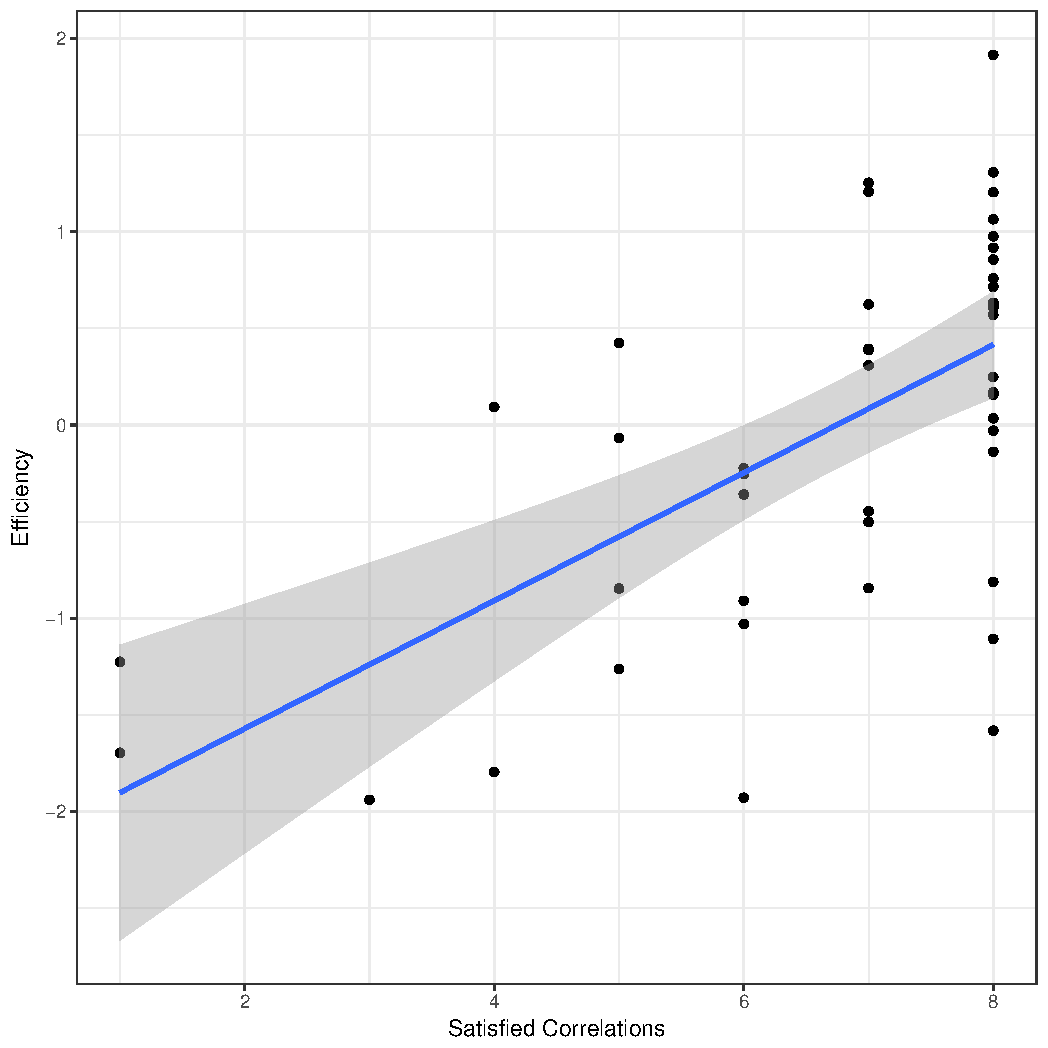
\includegraphics[width=.3\textwidth]{../results/correlations/correlations-by-grammar/ground-corrs-efficiency.pdf}
    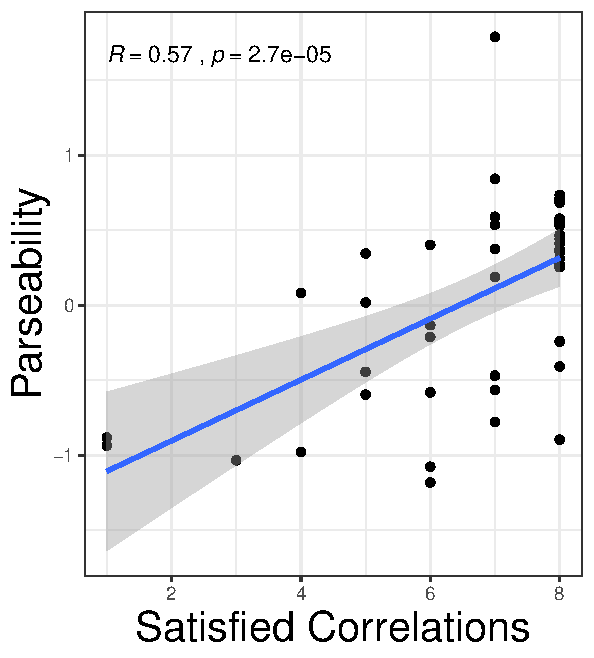
\includegraphics[width=.3\textwidth]{../results/correlations/correlations-by-grammar/ground-corrs-parseability.pdf}
    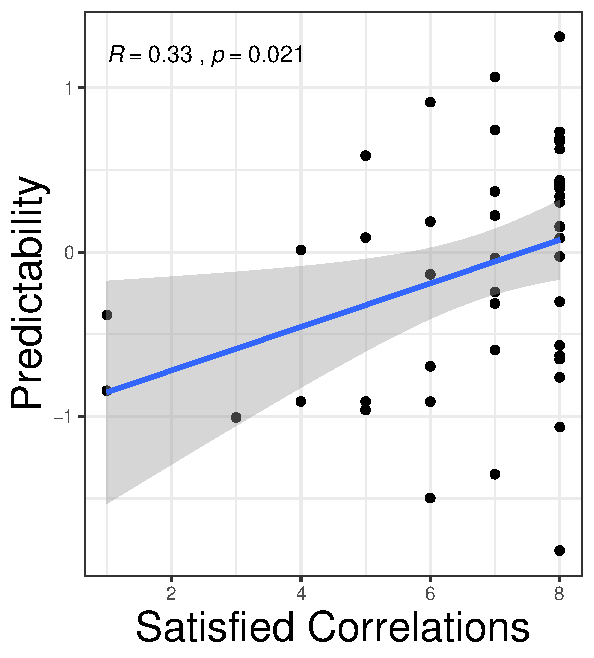
\includegraphics[width=.3\textwidth]{../results/correlations/correlations-by-grammar/ground-corrs-predictability.pdf}

	\caption{Correlation between the number of satisfied correlations ($x$-axis) and efficiency, parseability, and predictability ($y$-axis), for the 51 real languages.}
    \label{fig:corr-eff-corr}
\end{figure}



\subsection{Predictions for Individual Languages}


We show predictions for the eight correlations on the level of individual languages in Figure~\ref{fig:per-lang}.
We obtained these predictions for individual languages and each of the eight relations as follows.
For each language and each of the objective functions (efficiency, predictability, parseability), we considered the optimized grammar that yielded the best value of this objective function among the eight optimized grammars (i.e., the grammar where the optimization procedure had been most successful).
We interpreted this grammar as verb-object or object-verb depending on the order in the real grammar of the language.


\begin{figure} 
	\begin{center}
	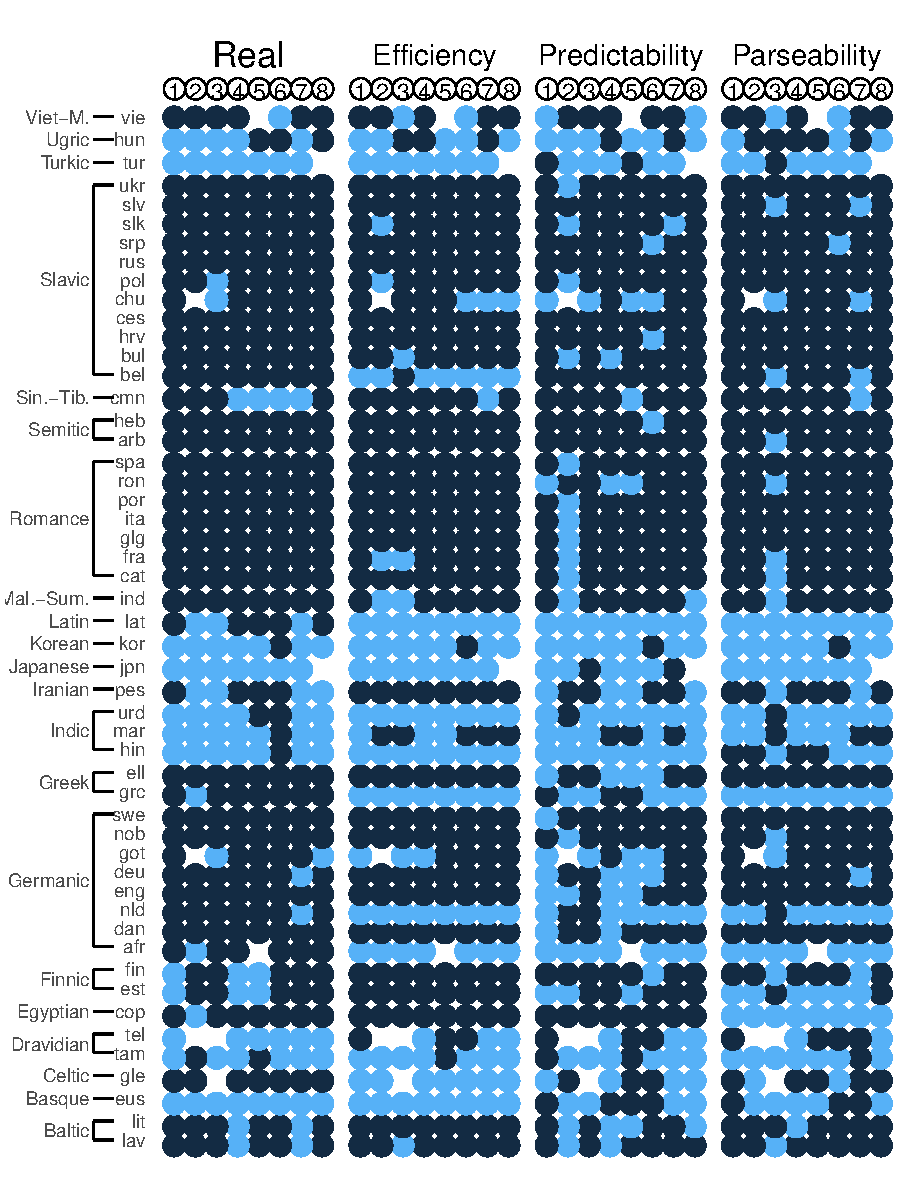
\includegraphics[width=0.7\textwidth]{../results/correlations/figures/pred-eff-pred-pars-families-2.pdf} 
	\end{center}
	\caption{Order of the eight correlates across 51 languages, in the real grammars (left) and predicted by optimizing for efficiency, predictability, parseability (right). Dark blue: Verb patterner \emph{precedes} object patterner (English, Arabic, ...). Light blue: Verb patterner \emph{follows} object patterner (Japanese, Hindi , ...). White cells indicate that the relation is not annotated in the dataset for the given language.}\label{fig:per-lang}
\end{figure}

\subsection{Regression for Predicted Correlations}


%https://github.com/stan-dev/stan/wiki/Prior-Choice-Recommendations

\paragraph{Bayesian Mixed-Effects Regression}
We modeled the probabilities $p_{L,j}$ that a grammar optimized for data from language $L$ satisfies the $j$-th correlation ($j=1,...,8$) using a multilevel logistic model \cite{gelman2013bayesian}, with random intercepts for the language for whose data the grammar had been optimized, and for its language family, annotated according to \url{http://universaldependencies.org/}.
Formally,
\begin{equation}\label{eq:mixed-effects}
logit(p_{L,j}) = \alpha_j + u_{L,j} + v_{f_L,j}
\end{equation}
where $f_L$ is the language family of $L$.
The intercepts $\alpha_j$ ($j=1,...8$) encode the population-level prevalence of the correlations when controlling for differences between datasets from different languages and language families; $u_{L,j}$, $v_{f_L,j}$ encode per-language and per-family deviations from the population-level intercept $\alpha_j$.



Following the recommendations of \cite{ghosh2018use, burkner2018advanced}, we used as a very weakly informative prior a Student's $t$ prior with $\nu=3$ degrees of freedom, mean 0, and scale $\sigma=10$ (i.e., the PDF $p$ is $\frac{1}{\sigma} p_3(x/\sigma)$, where $p_3$ is the PDF of the $t$-distribution with $\nu=3$).
We used this prior for $\alpha_j, \sigma_{L,j}, \tau_{L,j}$.
A correlation that holds in 90\% of cases would correspond to an intercept $\alpha \approx 2.19$ in the logistic model, well within the main probability mass of the prior.

We modeled full covariance matrices of per-language and per-family random intercepts over all eight correlations. We placed an LKJ prior ($\eta=1$) on these matrices, as described in \cite{burkner2018advanced}.
We used MCMC sampling implemented in Stan \cite{carpenter2017stan, hoffman2014no} using the R package \texttt{brms} \cite{buerkner2017brms}.
We ran four chains, with 5000 samples each, of which the first 2500 were discarded as warmup samples.
We confirmed convergence using $\hat{R}$ and visual inspection of chains \cite{gelman2013bayesian}.

We obtained the posterior density plots in Table 2 (Main Paper) and in Figure (\ref{tab:all-predictions-1}) by applying the logistic transformation ($x \mapsto \frac{1}{1+\exp(-x)}$) to the posterior samples of $\alpha_j$ (\ref{eq:mixed-effects}).
As the logistic transformation is inverse to the logit transform (\ref{eq:mixed-effects}), this corresponds to the posterior distribution of the prevalence (between 0.0 and 1.0) of each correlation, controlling for languages and language families.






\paragraph{Robustness}
To ascertain the robustness of our results, we also conducted a frequentist analysis using \texttt{lme4} \cite{bates2015fitting}.
For each of the correlations, we conducted a logistic mixed-effects analysis predicting whether a grammar satisfies the correlation, with random effects of language and language family.
The results are shown in Table~\ref{tab:corr-regression} together with those of the Bayesian analysis.
The frequentist analysis agrees with the Bayesian model; all eight correlations are predicted to hold in more than half of the optimized grammars ($p < 0.01$ each).

Note that the Bayesian analysis  also estimates a posterior distribution of the number of satisfied correlations (see Figure~\ref{fig:posterior}), providing an elegant solution to the multiple-comparisons problem arising from analysing the eight correlation.



\begin{table}
\small{
\begin{center}
\begin{tabular}{|l||l|lll|llll|ll|llllll}
\hline
 & Prevalence & \multicolumn{3}{c|}{Bayesian} & \multicolumn{4}{c|}{Frequentist} \\ 
& & Mean & SD & $p(\beta \leq 0)$ & $\beta$ & SE & $z$ & p \\
\hline\hline
	\raisebox{.5pt}{\textcircled{\raisebox{-.9pt} {1}}} & 0.779 & 1.449 & 0.273 & $<$ \num{1e-4} & 1.395 & 0.222 & 6.277 & \num{3.5e-10}\\
\raisebox{.5pt}{\textcircled{\raisebox{-.9pt} {2}}} & 0.678 & 0.761 & 0.171 & \num{1.0e-04} & 0.784 & 0.135 & 5.796 & \num{6.8e-09}\\
\raisebox{.5pt}{\textcircled{\raisebox{-.9pt} {3}}} & 0.696 & 1.003 & 0.424 & 0.012 & 0.943 & 0.342 & 2.753 & 0.006\\
\raisebox{.5pt}{\textcircled{\raisebox{-.9pt} {4}}} & 0.782 & 1.586 & 0.318 & $<$ \num{1e-4} & 1.512 & 0.251 & 6.013 & \num{1.8e-09}\\
\raisebox{.5pt}{\textcircled{\raisebox{-.9pt} {5}}} & 0.793 & 1.505 & 0.327 & $<$ \num{1e-4} & 1.434 & 0.272 & 5.281 & \num{1.3e-07}\\
\raisebox{.5pt}{\textcircled{\raisebox{-.9pt} {6}}} & 0.757 & 1.133 & 0.43 & 0.006 & 1.072 & 0.352 & 3.041 & 0.002\\
\raisebox{.5pt}{\textcircled{\raisebox{-.9pt} {7}}} & 0.748 & 1.093 & 0.388 & 0.003 & 1.026 & 0.322 & 3.185 & 0.001\\
\raisebox{.5pt}{\textcircled{\raisebox{-.9pt} {8}}} & 0.911 & 3.854 & 0.878 & $<$ \num{1e-4} & 3.823 & 0.782 & 4.887 & \num{1.0e-06}\\

\hline
\end{tabular}
\end{center}
}
	\caption{Detailed results for Bayesian and Frequentist mixed-effects analyses for the eight correlations. 
We show (1) the raw prevalence of each correlation in the optimized grammars (8 grammars for each of the 51 languages),
(2) for the Bayesian analysis, we provide posterior mean and SD of $\beta$, and the posterior probability that $\beta$ has the opposite sign,
(3) for the Frequentist analysis, we provide the point estimate, SE, $z$, and $p$-values (2-sided).
The frequentist analysis confirms the results of the Bayesian analysis.
}\label{tab:corr-regression}
\end{table}





\subsection{Comparing Efficiency to its Components}\label{sec:posterior-number}


In Figure~\ref{fig:posterior}, we plot the posterior distribution of the number of correlations predicted to hold in most optimized grammars, as obtained from the Bayesian regression.
For each posterior sample, we say that the $j$-th correlation holds if the value of $\alpha_j$ in that posterior sample is positive.
In the figure, we plot the fraction of posterior samples in which a given number of correlations is satisfied.
In addition to grammars optimized for efficiency, we also report the result for grammars optimized for predictability and for parseability alone.
Efficiency predicts all eight correlations with high posterior probability; predictability and parseability alone do not.

\begin{figure}[ht]
	\begin{center}
	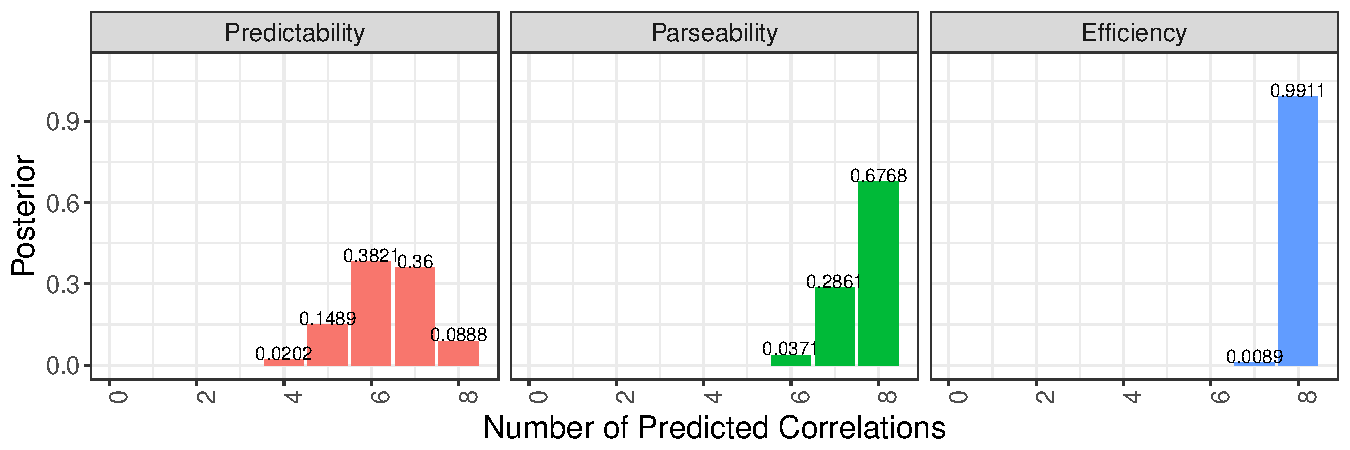
\includegraphics[width=0.98\textwidth]{../results/correlations/figures/posterior-satisfied-universals-together-large-three.pdf}
	\end{center}
	\caption{Posterior of the number of correlations correctly predicted by efficiency and its components, in the Bayesian multivariate mixed-effects logistic regression with random effects for languages and language families. We show results for grammars optimized for only Predictability (left), only Parseability (center), and full Efficiency (right).}\label{fig:posterior}
\end{figure}




\subsection{Results on all UD Relations}
In this section, we provide the predicted prevalence of correlations between the \emph{obj} dependency and all UD dependency types, along with the expected prevalence according to typological studies.
We also report results for grammars optimized for predictability and parseability individually.


We considered all UD syntactic relations occurring in at least two of the 51 languages.
In Table~\ref{tab:all-predictions-1}, we present the data for the eight correlations discussed in the main paper, and for those other relations for which the typological literature provides data.\footnote{The \emph{aux} syntactic relation in UD has the auxiliary (verb-patterner) as its dependent, and has direction \emph{opposite} to the auxiliary-verb relation \raisebox{.5pt}{\textcircled{\raisebox{-.9pt} {3}}}. Therefore, this relation is \emph{anti-correlated} with the verb-object relation, while \raisebox{.5pt}{\textcircled{\raisebox{-.9pt} {3}}} is \emph{correlated}.  For simplicity, we display this as a corelation in this table.}
Additionally, in Table~\ref{tab:all-predictions-2} we present data for the other UD relations, for which either no typological data is available, or which are not linguistically meaningful.





\begin{table*} 
	\begin{center}	
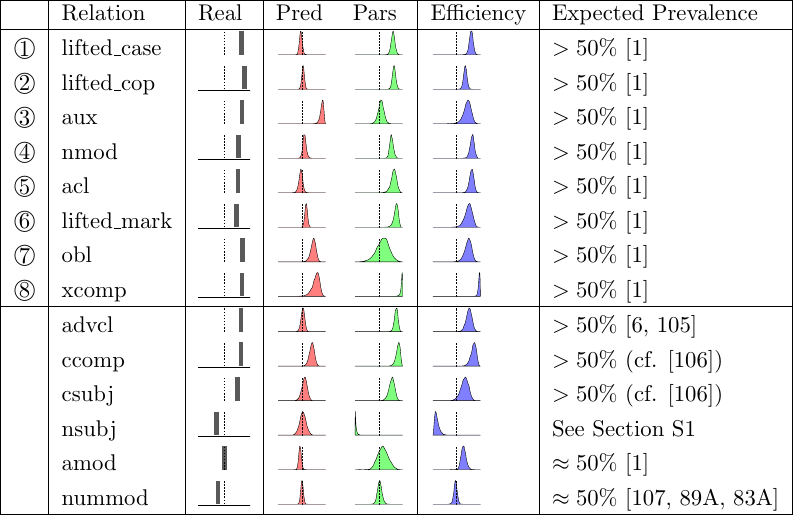
\includegraphics[width=0.8\textwidth]{si-table-perrel-1a-1.png}
\end{center}
\caption{Predictions on UD relations with predictions from the typological literature.
The first section contains the eight correlations discussed in the main paper (See Section~\ref{sec:correlations}); the second section provides other relations for which predictions are available.
The `Real' column provides the prevalence among the 51 languages in the Universal Dependencies data.
We provide posterior prevalences for grammars optimized for Efficiency, and for grammars optimized for Pars(eability) and Pred(ictability) alone, obtained from the Bayesian mixed-effects analysis controlling for languages and language families (as in Table 2 of the main paper).
In the last column, we indicate what prevalence is expected according to the typological literature. 
}
\label{tab:all-predictions-1}
\end{table*}





\begin{table*} 
	\begin{center}	
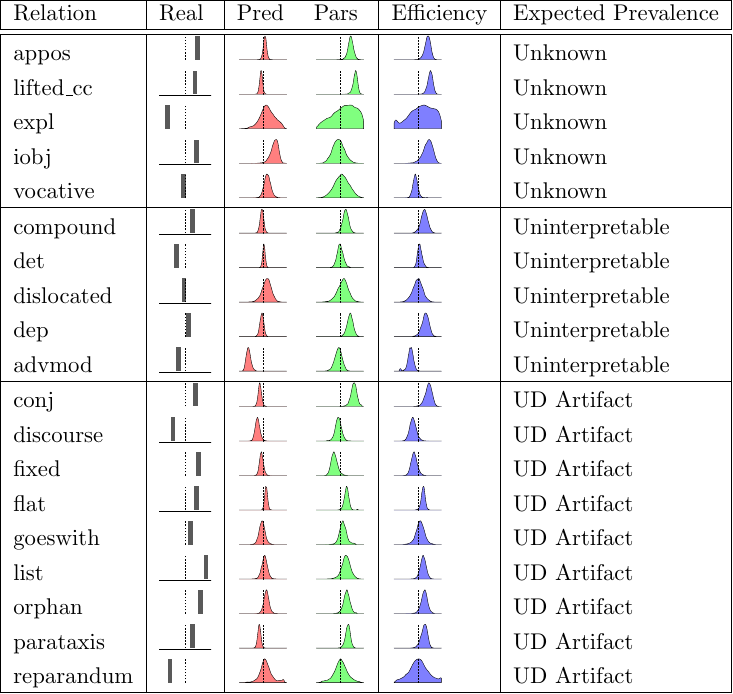
\includegraphics[width=0.7\textwidth]{si-table-perrel-2a-1.png}  
\end{center}
\caption{Predictions on UD relations for which no predictions are available in the typological literature.  ``Uninterpretable'' UD relations are those which collapse so many different linguistic relationships that they are not linguistically meaningful. ``UD artifact'' relations are those whose order is determined strictly by UD parsing standards, such that their order is not linguistically meaningful: these include dependencies such as the connection between two parts of a word that have been separated by whitespace inserted as a typo (\emph{goeswith}).
We provide results for grammars optimized for Efficiency, and for grammars optimized for Pars(eability) and Pred(ictability) alone.
}
\label{tab:all-predictions-2}
\end{table*}








\subsection{Previous Experiments}\label{sec:previous-exps}
In Table~\ref{table:corr-resu-previous} we report the results of our two previous, preregistered, simulations\footnote{\url{http://aspredicted.org/blind.php?x=8gp2bt}, \url{https://aspredicted.org/blind.php?x=bg35x7}. For the results of the Locality simulations described in the first preregistration, see the Dependency Length Minimization results in Table~\ref{tab:all-predictions-1b}, with discussion in Section~\ref{sec:DLM}.} together with results from the main experiment.
These experiments all had the same setup described in Section~\ref{sec:neural-architectures}, which was fixed before starting simulations; differences are that (1) one simulation places fully equal weight on parseability and predictability ($\lambda=1.0$), and (2) the final experiment uses three random seeds per grammar.
Results across all three experiments agree; jointly optimizing grammars for parseability and predictability produces all eight correlations.


\begin{table}[hbt!]

	\begin{center}
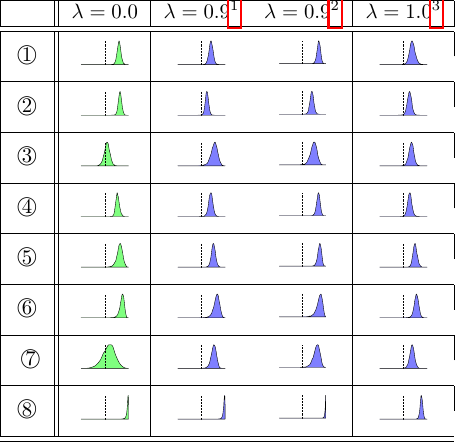
\includegraphics[width=0.4\textwidth]{si-table-perrel-3-1.png}  
\end{center}

	\begin{center}
\begin{tabular}{cccc}
$\lambda=0.0$ & $\lambda=0.9$ & $\lambda=0.9$ & $\lambda=1.0$ \\
	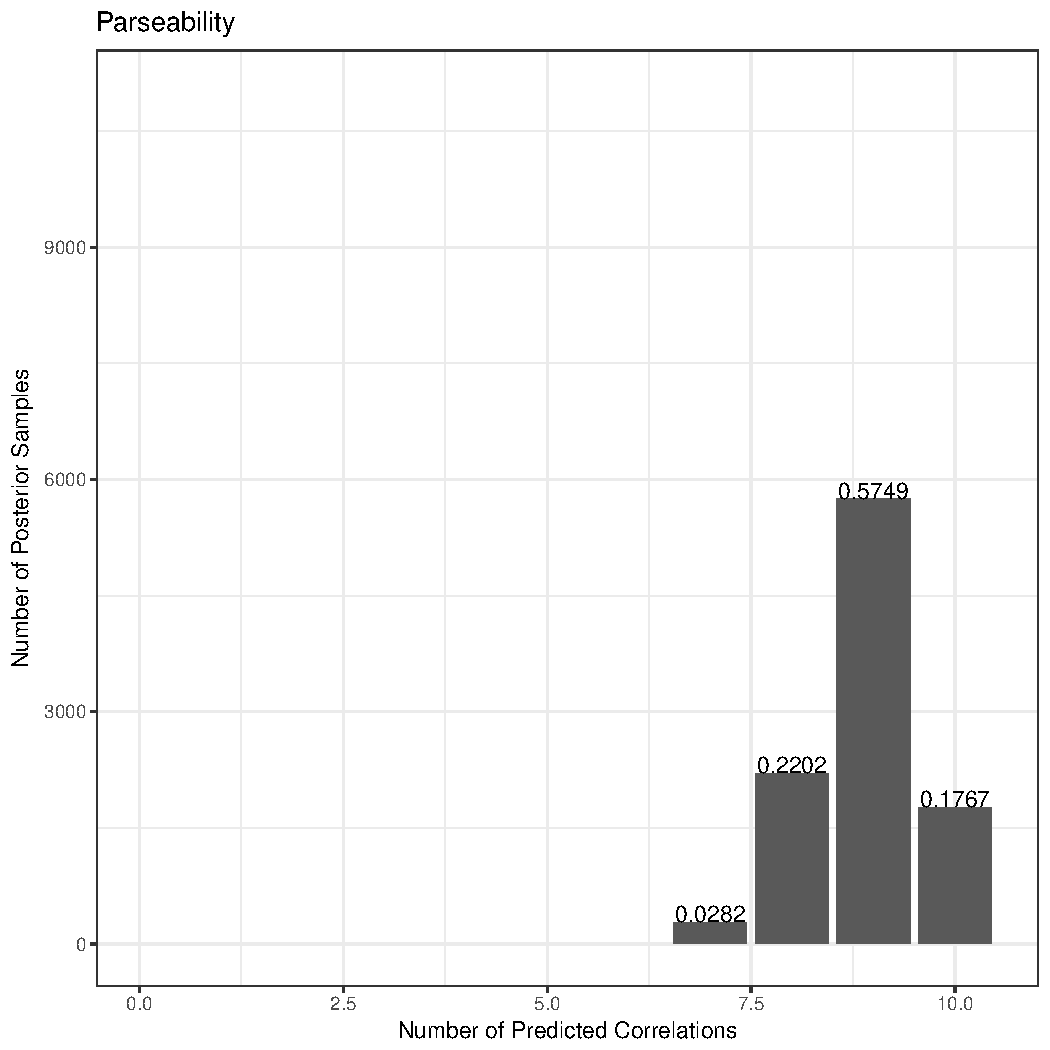
\includegraphics[width=0.15\textwidth]{../results/correlations/figures/posterior-satisfied-universals-parseability.pdf}&
	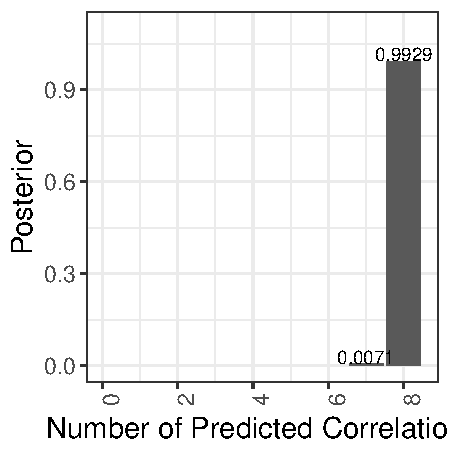
\includegraphics[width=0.15\textwidth]{../results/correlations/figures/posterior-satisfied-universals-together-large-prior-efficiency09.pdf}&
	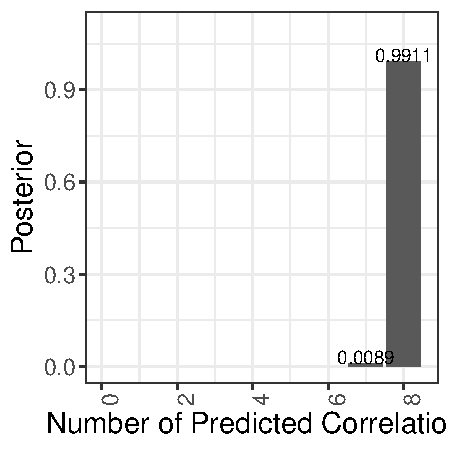
\includegraphics[width=0.15\textwidth]{../results/correlations/figures/posterior-satisfied-universals-efficiency-large.pdf}&
	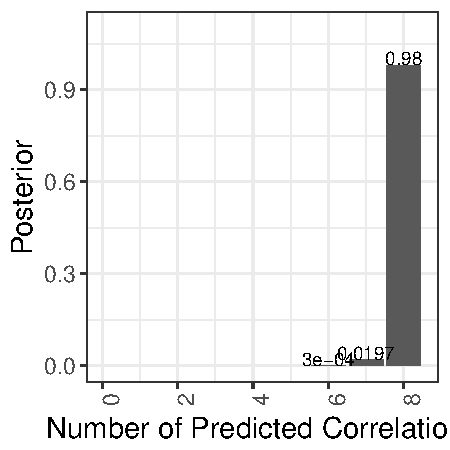
\includegraphics[width=0.15\textwidth]{../results/correlations/figures/posterior-satisfied-universals-together-large-prior-efficiency10.pdf}
\end{tabular}
	\end{center}
	\caption{Results from optimization experiments for different values of $\lambda$, including our two previous preregistered experiments (Section~\ref{sec:previous-exps}). For comparison, we also show results for $\lambda=0$, corresponding to optimizing for parseability only (same results as reported in Tables (\ref{tab:all-predictions-1}-\ref{tab:all-predictions-2})). For $\lambda=0.9$, we report results from one preliminary preregistered experiment (center left) and the final experiment (center right). For $\lambda=1.0$, we report the other preliminary preregistered experiment.
Giving similar weight to parseability and predictability -- that is, $\lambda$ close to $1$ -- results in more accurate word order predictions than choosing a small value of $\lambda$ such as $\lambda=0.0$. Note that $\lambda$ cannot take values smaller than zero, or greater than one, see Section \ref{sec:lambda}.
}\label{table:corr-resu-previous}
\end{table}



\subsection{Comparison to other Formalizations of Greenberg's Correlations}

We followed \citet{dryer1992greenbergian} in treating Greenberg's correlations as pairwise correlations with verb-object order.
While Greenberg's original study \cite{greenberg1963universals} also formalized most of these as correlations with verb-object order, a few were formalized as correlations between other relations that are only indirectly related to verb-object order (e.g., Universal 22 linking the position of the standard of comparison to the order of adpositions).

\citet{justeson1990explanation} conducted a log-linear analysis on typological judgments of 147 languages, constructing an undirected graphical model modeling correlations among any pair of six syntactic relations (verb-object, adposition-noun, noun-genitive, noun-relative clause, noun-adjective, verb-subject).
Results from their analysis suggested that, while some relations are directly correlated with the verb-object order, whereas other relations are only indirectly correlated with it.
In particular, in their analysis, the noun-genitive relation (corresponding to Correlation \raisebox{.5pt}{\textcircled{\raisebox{-.9pt} {4}}} here) was not directly correlated with the verb-object correlation; instead, the typologically observed correlation was explained through correlations between the noun-genitive relation and other relations (such as the adposition-noun relation) that directly correlate with the verb-object relation.
Note that this does not contradict the statement that verb-object and noun-genitive relations correlate; it shows that the observed correlation can be explained through a chain of other correlations.

Since the set of syntactic relations examined here is different from that examined by \citet{justeson1990explanation}, we cannot directly compare the predictions of efficiency optimization with their results.
Nonetheless, we can show that efficiency optimization is compatible with a picture of Greenberg's correlation as a network of pairwise correlations among different syntactic relations, and in particular the result that the correlation between the verb-object and noun-genitive relations is mediated through other correlations.

First, we directly test the optimized grammars for two additional correlations found by \citet{justeson1990explanation}:
For the relations examined here, beyond correlations with verb-object order, they found additional correlations between (1) the noun-genitive and adposition-noun dependencies, and (2) between the noun-relative clause and adposition-noun dependencies, \emph{beyond} the correlation mediated through the individual correlations with the verb-object dependency.
%With their model, they found no evidence for a direct correlation V-O, G-N beyond that mediated through other correlations.
We ran the same Bayesian logistic mixed-effects analysis for these two correlations.
Results are shown in Figure~\ref{tab:corr-regression-implication}.
Both correlations are very strongly supported by grammars optimized for efficiency.

Second, we directly applied the log-linear analysis described by \citet{justeson1990explanation} to optimized grammars.
We represent each grammar via the directions $v_1, \dots v_9$ of the nine relations indicated in Table 1 of the main paper (verb-object, and \raisebox{.5pt}{\textcircled{\raisebox{-.9pt} {1}}}-\raisebox{.5pt}{\textcircled{\raisebox{-.9pt} {8}}}), we coded these as $-0.5$ for Japanese-like order, and $+0.5$ for Arabic-like order.
This analysis models the relative frequency $p_{(v_1, \dots, v_9)}$ of a particular configuration of such a configuration $(v_1, \dots, v_9)$ by a log-linear model:
\begin{equation}
	\log p_{(v_1, \dots, v_9)} = u_0 + \sum_{i=1}^9 u_i v_i + \sum_{i, j \in C} u_{i,j} v_{i} v_{j}
\end{equation}
where $C$ is some set of (unordered) pairs of relations $\in \{1, \dots, 9\}$, modeling those pairs of relations that directly correlate with each other, and where $u_0, i_i, i_{i,j}$ are real-valued parameters.
For instance, if all relations directly correlate with the verb-object order, and not with any other relation, $C$ would contain all the unordered pairs containing the verb-object relation.

We inferred the best-fitting such model by selecting the pairs in $C$ via forward-selection using AIC.
The best-fitting model includes a set $C$ of 13 correlating pairs, with $AIC=274.18$.
This resulting model is shown in Figure~\ref{fig:loglinear}; following \cite{justeson1990explanation}, we show those links between nodes that are included in this selected model.
In agreement with the results of \cite{justeson1990explanation}, a network is identified in which all relations are connected at least indirectly, but several relations are not directly connected to the verb-object relation:
In particular, in accordance with the typological data analysed by \cite{justeson1990explanation}, the observed correlation between the verb-object and noun-genitive relation is entirely mediated through correlations with other relations (adposition-noun and verb-adpositional phrase) that directly correlate with the verb-object relation.
A difference is that, in our analysis and unlike the analysis by \cite{justeson1990explanation}, the noun-relative clause dependency is not directly linked to the verb-object relation; this might be because our analysis takes a different set of relations into account compared to \cite{justeson1990explanation}.


We also note that, unlike our mixed-effects models, this log-linear model does not have random effects, as we found that adding random effects to the log-linear model led to nonconvergence.
This means that it does not account for differences in the tree structures between languages and language families; as a result, the mixed-effects analyses for individual correlation pairs may be more conservative than this log-linear model.
Future work should replicate the analysis of \cite{justeson1990explanation} on a larger typological database and with more relations, to enable a direct comparison with the network structure predicted by  efficiency optimization.


\begin{table}
\small{
\begin{center}
\begin{tabular}{|ll||l|lll|llll|ll|llllll}
\hline
	& &Prevalence & Mean & SD & $p(\beta \leq 0)$  \\
\hline\hline
	G-N (nmod) & N-Adp (lifted\_case)  & 0.919 & 4.482 & 1.058 & $<$ \num{1e-4} \\
	Rel-N (acl) & N-Adp (lifted\_case) & 0.898 & 4.653 & 1.286 & $<$ \num{1e-4} \\
\hline
\end{tabular}
\end{center}
}
	\caption{Detailed results for the two correlations found by \citet{justeson1990explanation} that do not involve the verb-object dependency, for grammars optimized for efficiency. Both correlations are strongly supported by optimized grammars, holding in about 90\% of optimized grammars. Compare Table~\ref{tab:corr-regression}.
}\label{tab:corr-regression-implication}
\end{table}


\begin{figure}
	\begin{center}
	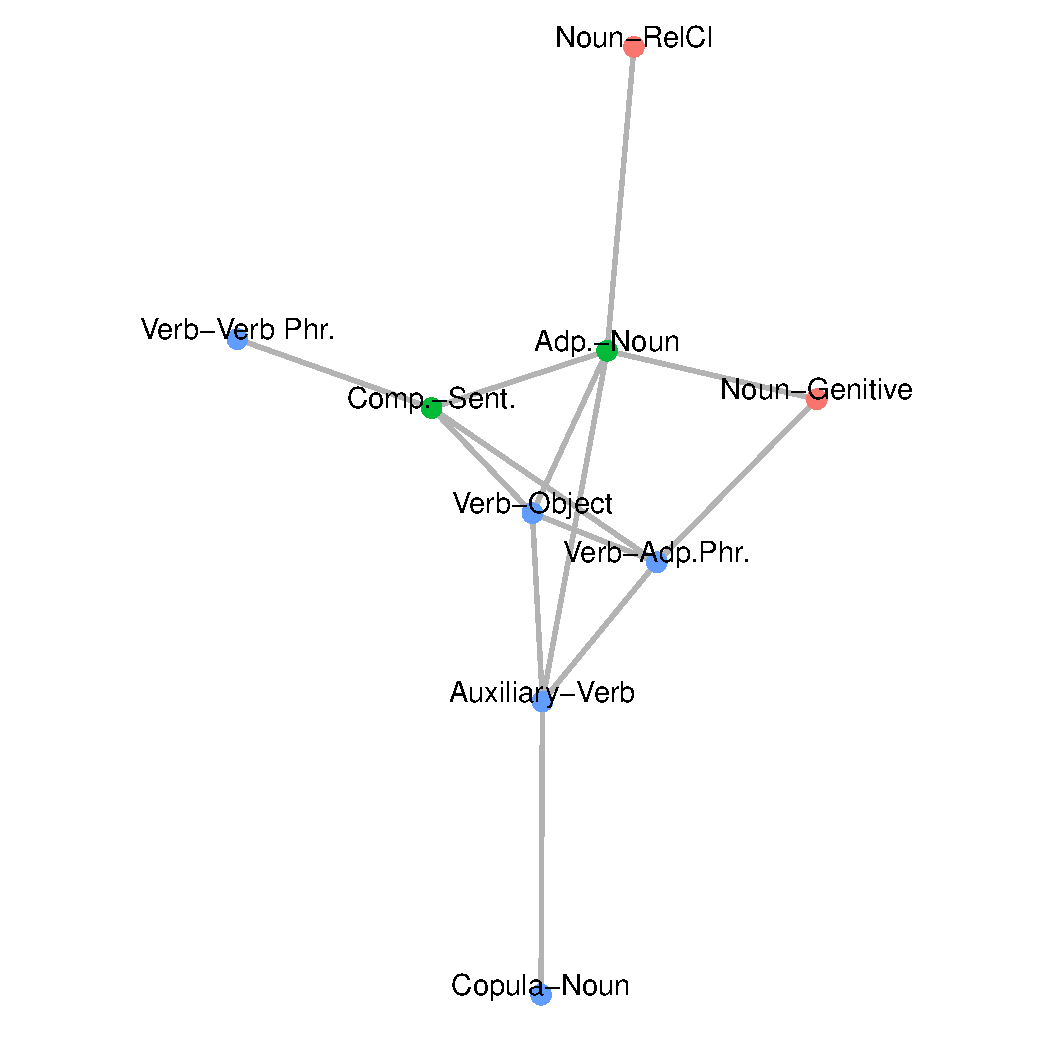
\includegraphics[width=0.8\textwidth]{../results/correlations/analysis/controls/loglinear-pairwise-correlations.pdf}
	\end{center}
	\caption{Network of pairwise correlations among the nine syntactic relations examined in this study, estimated from grammars optimized, identified using a log-linear model following \citet{justeson1990explanation}. The verb-object relation is at the center of the network. Relations between verbs and their dependents are colored in blue; relations between nouns and their dependents are colored in red; other relations are colored in green.}\label{fig:loglinear}
\end{figure}




\section{Creating Optimized Grammars}

In this section, we describe the method we employ for creating grammars that are optimized for efficiency, and how we extract grammars describing the actual ordering rules of languages.
%Our method will be applicable more generally to the task of optimizing grammars for a broad class of objective functions.
We carry out grammar optimization in an extended space of grammars that interpolates continuously between different grammars (Section~\ref{sec:diff-gramm}).
More specifically, we include probabilistic relaxations of grammars, which describe probability distributions over different ways of ordering a syntactic structure into a sentence.
This makes efficiency a \emph{differentiable} function of the grammar parameters, and enables efficient optimization with stochastic gradient descent, as we describe in Section~\ref{sec:optim-eff}.

This method addresses a major challenge noted in previous work optimizing grammars, namely that the predictability (and parseability) of an individual sentence depends on the entire distribution of the language.
Previously, \citet{gildea2015human} optimized grammars for dependency length and trigram surprisal using a simple hill-climbing method on the grammar parameters, which required reestimating the trigram surprisal model in every iteration.
Such a method would be computationally prohibitive for efficiency optimization, as it would require reestimating the neural network models after every change to the grammar, which would amount to reestimating them hundreds or thousands of times per grammar.
Our method, by allowing for the use of stochastic gradient descent, addresses this challenge, as we describe in Section~\ref{sec:optim-eff}.


\subsection{Differentiable Ordering Grammars}\label{sec:diff-gramm}

We extended the parameter space of grammars by continuously interpolating between grammars, making efficiency a \emph{differentiable} function of grammar parameters.
The parameters of such a \key{differentiable word order grammar} are as follows. 
For each dependency label type $\tau$, we have (1) a \key{Direction Parameter} $a_\tau \in [0,1]$, and (2) a \key{Distance Parameter} $b_\tau \in \mathbb{R}$. 
Each dependent is ordered on the left of its head with probability $a_\tau$ and to the right with probability $1-a_\tau$. 
Then for each set of co-dependents $\{s_1, \dots , s_n\}$ placed on one side of a head, their order from left to right is determined by iteratively sampling from the distribution $\operatorname{softmax}(b_{\tau_1}, \dots, b_{\tau_n})$ (for dependents preceding the head) or $\operatorname{softmax}(-b_{\tau_1}, \dots, -b_{\tau_n})$ (for dependents following the head) (for the definition of $\operatorname{Softmax}$, see \cite[p. 184]{goodfellow2016deep}) without replacement.

If $a_\tau \in \{0, 1\}$, and the distances between values of $b_\tau$ (for different $\tau$) become very large, such a differentiable grammar becomes deterministic, assigning almost full probability to exactly one ordering for each syntactic structure.
In this case, the grammar can be converted into an equivalent grammar of the form described in Materials and Methods, by extracting a single parameter in $[-1, 1]$ for each relation $\tau$.

We provide an example in Figure~\ref{fig:grammar-sample}, illustrating grammar parameters for the relations in Figure 3 of the main paper.

Note that the grammatical formalism simplifies some aspects of the word order regularities of natural languages.
For instance, it does not represent cases where ordering varies between main and embedded clauses, as it does not condition ordering decisions on the larger context.
It also does not nonprojective orderings, which -- while generally rare -- do occur in many languages (CITE).
More complex and powerful ordering grammar models have been proposed \cite{futrell2015experiments, wang2016galactic}; however, they have similar limitations, and for our purposes, the model adopted here has the advantage of being simple and interpretable.



\begin{figure}
	\begin{center}
\begin{tabular}{l||l|ll||l|lllll}
	& \multicolumn{3}{c||}{English}    &  \multicolumn{3}{c}{Japanese}  \\ 
	Relation                     &  Par.   & $a_\tau$ & $b_\tau$            & Par.   & $a_\tau$ & $b_\tau$     \\ \hline \hline
	object (\textit{obj})        &  $0.1$   &   $0.04$   & $-1.46$            & $-0.1$  & $0.99$ & $-0.7$2 \\
	oblique (\textit{obl})       &  $0.3$   &   $0.13$     & $1.25$             & $-0.3$  & $0.99$ & $0.73$ \\
	case (\textit{lifted\_case}) &  $0.2$   &   $0.07$       &   $-0.89$         & $-0.2$  &  $0.92$ & $0.02$  \\
\end{tabular}
	\end{center}
	\caption{Sample Coefficients from grammars extracted from the real English and Japanese orderings (Section~\ref{sec:extract-grammars}), for the relations occurring in Figure 3 (Main Paper). We show parameters in $[-1,1]$ for deterministic word order grammars as described in \emph{Materials and Methods}, and the coefficients ($a_\tau, b_\tau$) for corresponding differentiable ordering grammars. For the deterministic grammars (`Par.'), positive coefficients indicate that the dependent will be placed after the head. For the differentiable grammars, $a_\tau > 0.5$ indicates predominance of ordering of dependents before heads, and larger $b_\tau$ indicates greater distance between head and dependent.}\label{fig:grammar-sample}
\end{figure}


\subsection{Extracting Grammars from Datasets}\label{sec:extract-grammars}
We extract grammars for each actual language by fitting a differentiable ordering grammar maximizing the likelihood of the observed orderings.
To prevent overfitting, we regularize each $a_\tau$, $b_\tau$ with a simple Bayesian prior $logit(a_\tau) \sim \mathcal{N}(0,1)$, $b_\tau \sim \mathcal{N}(0,1)$.
We implemented this regularized optimization as mean-field ELBO variational inference in Pyro~\cite{bingham2018pyro}.
We then extract the posterior means for each parameter $a_\tau, b_\tau$, and convert the resulting differentiable grammar into an ordinary ordering grammar.




We validated the extracted grammars by comparing the dominant orders of six syntactic relations that are also annotated in the World Atlas of Linguistic Structures (WALS, \cite{haspelmath2005world}).
Among the eight Greenbergian correlations that we were able to test, five are annotated in WALS: adpositions, complementizers, relative clauses, genitives, and oblique PPs.
In Table~\ref{tab:grammars-wals}, we compare our grammars with WALS on these five relations, and the verb-object relation.
WALS has data for 74\% of the entries\footnote{Serbian and Croatian are listed as a single language Serbian-Croatian in WALS. In the table, we compare those with the grammar we extracted for Croatian, noting that it fully agrees with the Serbian grammar.}, and lists a dominant order for 91\% of these.
The grammars we extracted from the corpora agree with WALS in 96~\%  of these cases.




\begin{table}
\small{
\begin{center}
\begin{tabular}{l||ll|ll|ll|ll|ll|ll|llllll}
		   Language 
		   &	\multicolumn{2}{c|}{Objects} 
		   &	\multicolumn{2}{c|}{Adpositions} 
		   &	\multicolumn{2}{c|}{Compl.} 
		   &	\multicolumn{2}{c|}{Rel.Cl.} 
		   &	\multicolumn{2}{c|}{Genitive} 
		   &	\multicolumn{2}{c|}{PP}  \\ \hline\hline
	Afrikaans  & DH  & ?  & HD  & ?  & HD  & ?  & --  & ?  & HD  & ?  & HD  & ?  & \\ 
Anc.Grk.  & DH  & ?  & HD  & ?  & HD  & ?  & HD  & ?  & HD  & ?  & HD  & ?  & \\ 
Arabic  & HD  & HD  & HD  & HD  & HD  & HD  & HD  & ?  & HD  & HD  & HD  & HD  & \\ 
Basque  & DH  & DH  & DH  & DH  & DH  & DH  & DH  & DH  & DH  & DH  & DH  & DH  & \\ 
Belarusian  & HD  & *  & HD  & ?  & HD  & ?  & HD  & HD  & HD  & HD  & HD  & *  & \\ 
Bulgarian  & HD  & HD  & HD  & HD  & HD  & HD  & HD  & HD  & HD  & *  & HD  & HD  & \\ 
Catalan  & HD  & HD  & HD  & HD  & HD  & ?  & HD  & HD  & HD  & HD  & HD  & ?  & \\ 
Chinese  & HD  & HD  & HD  & *  & DH  & ?  & DH  & DH  & DH  & DH  & DH  & DH  & \\ 
Coptic  & HD  & HD  & HD  & HD  & HD  & HD  & HD  & HD  & HD  & HD  & HD  & HD  & \\ 
Croatian  & HD  & HD  & HD  & HD  & HD  & HD  & HD  & ?  & HD  & *  & HD  & ?  & \\ 
Czech  & HD  & HD  & HD  & HD  & HD  & HD  & HD  & HD  & HD  & *  & HD  & ?  & \\ 
Danish  & HD  & HD  & HD  & HD  & HD  & HD  & HD  & HD  & \textit{HD} & DH  & HD  & HD  & \\ 
Dutch  & DH  & *  & HD  & HD  & HD  & HD  & HD  & HD  & HD  & HD  & DH  & *  & \\ 
English  & HD  & HD  & HD  & HD  & HD  & HD  & HD  & HD  & HD  & *  & HD  & HD  & \\ 
Estonian  & HD  & HD  & DH  & DH  & HD  & HD  & \textit{DH} & HD  & DH  & DH  & HD  & HD  & \\ 
Finnish  & HD  & HD  & DH  & DH  & HD  & HD  & \textit{DH} & HD  & DH  & DH  & HD  & HD  & \\ 
French  & HD  & HD  & HD  & HD  & HD  & HD  & HD  & HD  & HD  & HD  & HD  & HD  & \\ 
Galician  & HD  & ?  & HD  & ?  & HD  & ?  & HD  & ?  & HD  & ?  & HD  & ?  & \\ 
German  & HD  & *  & HD  & HD  & HD  & HD  & HD  & HD  & HD  & HD  & DH  & *  & \\ 
Gothic  & HD  & ?  & HD  & ?  & HD  & ?  & HD  & ?  & HD  & ?  & HD  & ?  & \\ 
Greek  & HD  & HD  & HD  & HD  & HD  & HD  & HD  & HD  & HD  & HD  & HD  & ?  & \\ 
Hebrew  & HD  & HD  & HD  & HD  & HD  & HD  & HD  & HD  & HD  & HD  & HD  & ?  & \\ 
Hindi  & DH  & DH  & DH  & DH  & HD  & HD  & DH  & *  & DH  & DH  & DH  & ?  & \\ 
Hungarian  & \textit{DH} & HD  & DH  & DH  & HD  & HD  & HD  & *  & DH  & DH  & DH  & ?  & \\ 
Indonesian  & HD  & HD  & HD  & HD  & HD  & HD  & HD  & HD  & HD  & HD  & HD  & HD  & \\ 
Irish  & HD  & HD  & HD  & HD  & HD  & HD  & HD  & HD  & HD  & HD  & HD  & HD  & \\ 
Italian  & HD  & HD  & HD  & HD  & HD  & HD  & HD  & HD  & HD  & HD  & HD  & ?  & \\ 
Japanese  & DH  & DH  & DH  & DH  & DH  & DH  & DH  & DH  & DH  & DH  & DH  & DH  & \\ 
Korean  & DH  & DH  & DH  & DH  & \textit{HD} & DH  & DH  & DH  & DH  & DH  & DH  & ?  & \\ 
Latin  & DH  & ?  & HD  & ?  & HD  & ?  & HD  & ?  & HD  & ?  & DH  & ?  & \\ 
Latvian  & HD  & HD  & HD  & HD  & HD  & HD  & HD  & HD  & DH  & DH  & DH  & ?  & \\ 
Lithuanian  & HD  & HD  & HD  & HD  & HD  & HD  & HD  & HD  & DH  & DH  & DH  & ?  & \\ 
Marathi  & DH  & DH  & DH  & DH  & HD  & *  & DH  & DH  & DH  & DH  & DH  & ?  & \\ 
Norwegian  & HD  & HD  & HD  & HD  & HD  & HD  & HD  & HD  & HD  & *  & HD  & ?  & \\ 
O.C.Slav.  & HD  & ?  & HD  & ?  & HD  & ?  & HD  & ?  & HD  & ?  & HD  & ?  & \\ 
Persian  & DH  & DH  & HD  & HD  & HD  & HD  & HD  & HD  & HD  & HD  & DH  & ?  & \\ 
Polish  & HD  & HD  & HD  & HD  & HD  & HD  & HD  & HD  & HD  & HD  & HD  & ?  & \\ 
Portuguese  & HD  & HD  & HD  & HD  & HD  & ?  & HD  & HD  & HD  & HD  & HD  & ?  & \\ 
Romanian  & HD  & HD  & HD  & HD  & HD  & HD  & HD  & HD  & HD  & HD  & HD  & ?  & \\ 
Russian  & HD  & HD  & HD  & HD  & HD  & HD  & HD  & HD  & HD  & HD  & HD  & ?  & \\ 
Serbian  & HD  & ?  & HD  & ?  & HD  & ?  & HD  & ?  & HD  & ?  & HD  & ?  & \\ 
Slovak  & HD  & ?  & HD  & ?  & HD  & ?  & HD  & ?  & HD  & ?  & HD  & ?  & \\ 
Slovenian  & HD  & HD  & HD  & HD  & HD  & ?  & HD  & ?  & HD  & *  & HD  & ?  & \\ 
Spanish  & HD  & HD  & HD  & HD  & HD  & HD  & HD  & HD  & HD  & HD  & HD  & HD  & \\ 
Swedish  & HD  & HD  & HD  & HD  & HD  & HD  & HD  & HD  & \textit{HD} & DH  & HD  & HD  & \\ 
Tamil  & DH  & DH  & DH  & DH  & DH  & *  & \textit{HD} & DH  & DH  & DH  & DH  & DH  & \\ 
Telugu  & DH  & DH  & DH  & DH  & DH  & *  & DH  & DH  & DH  & DH  & DH  & ?  & \\ 
Turkish  & DH  & DH  & DH  & DH  & DH  & *  & DH  & DH  & DH  & DH  & DH  & DH  & \\ 
Ukrainian  & HD  & HD  & HD  & HD  & HD  & HD  & HD  & HD  & HD  & ?  & HD  & ?  & \\ 
Urdu  & DH  & DH  & DH  & DH  & HD  & HD  & HD  & *  & DH  & DH  & DH  & ?  & \\ 
Vietnamese  & HD  & HD  & HD  & HD  & \textit{DH} & HD  & --  & HD  & HD  & HD  & HD  & HD  & \\ 

\end{tabular}
\end{center}
}
\caption{Comparing grammars extracted from databases to linguistic judgments in the World Atlas of Linguistic Structures. For each of the six syntactic relation, the first column provides the ordered coded in the extracted grammar; the second column provides the order coded in WALS (DH for dependent-head, HD for head-dependent order). `?' indicates that WALS has no data.
$*$ indicates that WALS does not list a dominant order; as \citet{dryer2011evidence} describes, this can mean that neither order is dominant in the language, or that insufficient data was available when compiling WALS.
Finally, `--' indicates that the relation does not occur in the Universal Dependencies corpus.
}\label{tab:grammars-wals}
\end{table}




\subsection{Optimizing Grammars for Efficiency}\label{sec:optim-eff}

In this section, we describe how we optimized grammar parameters for efficiency.
A word order grammar can be viewed as a function $\mathcal{L}_\theta$, whose behavior is specified by parameters $\theta$, which takes an unordered dependency tree $t$ as input and produces as output an ordered sequence of words $u = \mathcal{L}_\theta(t)$ linearizing the tree.
More generally, if $\mathcal{L}_\theta$ is a differentiable ordering grammar (Section~\ref{sec:diff-gramm}), then $\mathcal{L}_\theta(t)$ defines a \emph{probability distribution} $p_{\mathcal{L}_\theta}(u|t)$ over ordered sequences of words $u$.
In the limit where $\mathcal{L}_\theta$ becomes deterministic, the distribution $p_{\mathcal{L}_\theta}(u|t)$ concentrates on a single ordering $u$.

Recall the definition of efficiency
\begin{equation}\label{eq:efficiency-recall}
	R_{\textit{Eff}} := R_{\textit{Pars}} + \lambda R_\textit{Pred},
\end{equation}
where
\begin{equation}\label{eq:rpars}
	R_{Pars} := \operatorname{I}[\utterance,\tree] = \sum_{t,u} p(t,u) \log \frac{p(t|u)}{p(t)} 
\end{equation}
\begin{equation}
	R_{Pred} := - \operatorname{H}[\utterance] = \sum_{u} p(u) \log p(u),
\end{equation}
where $t \sim \tree$ is the distribution over syntactic structures as found in databases of the language, and $u \sim p_{\mathcal{L}_\theta}(u|t)$ denotes the corresponding linearized sentences.

These quantities are estimated using two neural models, as described in Section~\ref{sec:neural-architectures}:
A \key{parser} recovers syntactic structures from utterances by computing a distribution $p_\phi(t|u)$, parameterized via parser parameters $\phi$.
The degree to which a parser with parameters $\phi$ succeeds in parsing a sentence $u$ with structure $t$ is\footnote{Note that, in the definition of $R_{Pars}$ (\ref{eq:rpars}), the term $p(t)$ is a constant independent of $\phi$ and the word order grammar $\mathcal{L}_\theta$; it can therefore be ignored in the optimization process.} 
\begin{equation}
	R_{Pars}^{\phi}(u,t) =  \log p_\phi(t|u).
\end{equation}
A \key{language model}, with some parameters $\psi$, calculates the word-by-word surprisal of an utterance:
\begin{equation}
	R_{Pred}^{\psi}(u) = \sum_{i=1}^{|u|} \log p_\psi(u_i|u_{1\dots i-1}).
\end{equation}
Using this and Gibbs' inequality~\cite{cover2006elements}, we can rewrite Efficiency~(\ref{eq:efficiency-recall}), for a given grammar $\theta$, equivalently into the parseability and predictability achieved with the best parser and language models:
\begin{equation}
	R_{\textit{Eff}}^{\theta} := \max_{\phi,\psi} R_{\textit{Eff}}^{\theta, \phi, \psi},
\end{equation}\label{eq:efficiency-rewrite}
where we have written
\begin{equation}
R_{\textit{Eff}}^{\theta, \phi, \psi} := \E_{t \sim \mathcal{T}} \E_{u \sim p_{\mathcal{L}_\theta}(u|t)} \left[R_{Pars}^{\phi}(u,t) + \lambda R_{Pred}^{\psi}(u)\right].
\end{equation}
In order to find an optimal grammar $\theta$, we thus need to compute 
\begin{equation}\label{eq:efficiency}
\argmax_\theta\	R_{\textit{Eff}}^{\theta} = \argmax_\theta\	\max_{\phi, \psi} R_{\textit{Eff}}^{\theta, \phi, \psi} 
%= \argmax_\theta\	\max_{\phi, \psi} \E_t \E_{u \sim p_\theta(u|t)} \left[R_{Pars}^{\phi}(u,t) + \lambda R_{Pred}^{\psi}(u)\right]
\end{equation}
Importantly, $R_{\textit{Eff}}^{\theta, \phi, \psi}$ is differentiable in $\theta, \phi, \psi$: %, and we can apply stochastic gradient descent to carry out this optimization.
\begin{align}
\partial_\theta R_{\textit{Eff}}^{\theta, \phi, \psi} &= \E_t \E_{u \sim p_{\mathcal{L}_\theta}(u|t)} \left[  \left[\partial_\theta \log p_{\mathcal{L}_\theta}(u|t)\right] \cdot    \left(R_{Pars}^{\phi}(u,t) + \lambda R_{Pred}^{\psi}(u)\right) \right] \label{eq:dtheta}\\ 
\partial_\phi R_{\textit{Eff}}^{\theta, \phi, \psi} &= \E_t \E_{u \sim p_{\mathcal{L}_\theta}(u|t)}  \left[\partial_\phi R_{Pars}^{\phi}(u,t)\right] \\
\partial_\psi R_{\textit{Eff}}^{\theta, \phi, \psi} &= \E_t \E_{u \sim p_{\mathcal{L}_\theta}(u|t)}  \left[\lambda \cdot \partial_\psi R_{Pred}^{\psi}(u)\right] \label{eq:dpsi},
\end{align}
where (\ref{eq:dtheta}) is derived using the \emph{score-function} or \emph{REINFORCE} theorem~\cite{williams1992simple}.
Note that the derivatives inside the expectations on the right hand sides can all be computed using backpropagation for our neural network architectures.

We can therefore apply stochastic gradient descent to jointly optimize $\theta, \phi, \psi$:
In each optimization step, we sample a dependency tree $t$ from the database, then sample an ordering from the current setting of $\theta$ to obtain a linearized sentence ${\bf w} \sim p_{\theta}(\cdot|t)$.
Then we %update $\thetal$ with ordinary gradient descent, and $\thetad$ with the REINFORCE estimator~\ref{williams-simple-1992}.
do a gradient descent step using the estimator given by the expressions in the square brackets in (\ref{eq:dtheta}-\ref{eq:dpsi}).


Optimizing for only parseability (or predictability) is very similar---in this case, the terms involving $R_{Pred}^\phi$ (or $R_{Pars}^\psi$) are removed.


At the beginning of the optimization procedure, we initialize all values $a_\tau := 0.5$, $b_\tau := 0$ (except for the \emph{obj} dependency, for which we fix $a_\tau$ to 0 or 1, see Section~\ref{sec:neural-architectures}).
The neural parser and language model are also randomly initialized at the beginning of optimization.
Empirically, we observe that optimizing differentiable ordering grammars for efficiency leads to convergence towards deterministic behavior, allowing us to extract equivalent deterministic grammars as described in Section~\ref{sec:diff-gramm}.

See Section~\ref{sec:neural-architectures}, paragraph `Optimization Details' for the stopping criterion and learning rates used in this optimization scheme.



\section{Neural Network Architectures}\label{sec:neural-architectures}

In this section, we describe the details of the neural network architectures.
Choices follow standard practice in machine learning.
All choices, except where explicitly noted otherwise, were made before evaluating word order properties, and the efficiency of real grammars.


\paragraph{Estimating Predictability}
We choose a standard LSTM language model \citep{goldberg2017neural, hochreiter1997long}, as such recurrent neural models are the strongest known predictors of the surprisal effect on human processing effort~\cite{frank2011insensitivity,goodkind2018predictive}.
This model uses a recurrent neural network to compute the predictability of a sentence $u = u_1...u_n$\footnote{Technically, $u_1...u_{n-1}$ are words, and $u_n$ is an end-of-sentence token, to ensure the probability distribution over all sentences is normalized.}:
\begin{equation}
\log p_\psi(u) = \sum_{i=1}^n \log p_\psi(u_i|u_{1\dots i-1})
\end{equation}
where $\psi$ are the parameters of the recurrent LSTM network, optimized on training data (see paragraph `Optimization Details').


We estimate the average predictability of a language as a Monte Carlo estimate on held-out data:
\begin{equation}
	R_{Pred} := - \operatorname{H}[\utterance] = \sum_{u} p(u) \log p_\psi(u) \approx \frac{1}{|\text{Heldout Data}|} \sum_{u \in \text{Heldout Data}} \log p_\psi(u)
\end{equation}
by averaging over all sentences $u$ occurring in the corpus.


For computational reasons, we restrict the vocabulary to the most frequent 50,000 words in the treebanks for a given language.
Given the moderate size of the corpora, this limit is only attained only for few languages.
In each time step, the input is a concatenation of embeddings for the word, for language-specific POS tags, and for universal POS tags.
The model predicts both the next word and its language-specific POS tag in each step.
Using POS tags is intended to prevent overfitting on small corpora.
This choice was made before evaluating the efficiency of real grammars, and before evaluating word order properties.


\paragraph{Estimating Parseability}
We use a biaffine attention parser architecture \citep{kiperwasser2016simple,zhang2017dependency,dozat2017stanford}. This architecture is remarkably simple: the words of a sentence are encoded into context-sensitive embeddings using bidirectional LSTMs, then a classifier is trained to predict the head for each work. The classifier works by calculating a score for every pair of word embeddings $(w_i, w_j)$, indicating the likelihood that the $j$th word is the head of the $i$th word. This is a highly generic architecture for recovering graph structures from strings, and is a simplification of graph-based parsers which reduce the parsing problem to a minimal spanning tree problem \citep{mcdonald2005nonprojective}.
The parseability of a sentence $u = u_1\dots u_n$ with syntactic structure $t$ is computed as
\begin{equation}
	\log p_\phi(t|u) = \sum_{i=1}^n \log p_\phi(\text{head}_i, \text{label}_i | u, i)
\end{equation}\label{eq:pars-obj}
where $\text{head}_i \in \{\textsc{root}, 1,\dots,n\}$ is the index of the head of $u_i$ in the syntactic structure, and $\text{label}_i$ is its syntactic relation as formalized in UD; $\phi$ denotes the parameters estimated on the training data (see paragraph `Optimization Details').
The overall parseability is estimated as a Monte Carlo estimate on held-out data:
\begin{equation}\label{eq:rpars}
	R_{Pars} := \operatorname{I}[\utterance,\tree] = \sum_{t,u} p(t,u) \log \frac{p_\phi(t|u)}{p(t)} = \frac{1}{|\text{Heldout Data}|} \sum_{t,u \in \text{Heldout Data}} \log \frac{p_\phi(t|u)}{p(t)}
\end{equation}
The constant $p(t)$ only depends on the language (but not on the word order rules), and can thus be ignored when comparing different grammars applied to the same language, and when optimizing grammars for a given language; we therefore do not attempt to explicitly estimate it.


To reduce overfitting on small corpora, we choose a delexicalized setup, parsing only from POS tags. Preliminary experiments showed that a parser incorporating word forms overfitted long before the ordering grammar had converged; parsing from POS tags prevents early overfitting.
This decision was made before evaluating word order properties.

\paragraph{Hyperparameters}
Neural network models have hyperparameters such as the number of hidden units, and the learning rate. 
For predictability and parseability optimization, we first selected hyperparameters on the respective objectives for selected languages on the provided development partitions.
These parameters are shown in Table~\ref{tab:hyperparameters}.
Then, for each language and each objective function, we created eight random combinations of these selected hyperparameter values, and selected the setting that yielded the best value of the respective objective function (efficiency, predictability, parseability) on the language. We then used this setting for creating optimized word order grammars. 




All word and POS embeddings are randomly initialized with uniform values from $[-0.01, 0.01]$.
We do not use pretrained embeddings \citep{peters2018deep}; while these could improve performance of language models and parsers, they would introduce confounds from the languages' actual word orders as found in the unlabeled data.


\begin{table}[]
    \centering
    \begin{tabular}{|l|l|l|}
\hline
\multirow{2}{*}{Optimization}&    Learning Rate     & 5e-6, 1e-5, 2e-5, 5e-5 \\
&    Momentum & 0.8, 0.9 \\ \hline
\multirow{6}{*}{Language Model} &    Learning Rate  & 0.5, 0.1, 0.2 \\
&    Dropout Rate& 0.0, 0.3, 0.5 \\
& Embedding Size (Words) & 50 \\
& Embedding Size (POS) & 20 \\
&    LSTM Layers  & 2 \\
&    LSTM Dimensions  & 128 \\
 \hline
\multirow{5}{*}{Parser}&    Learning Rate  & 0.001 \\
&    Dropout Rate  & 0.2 \\
&    Embedding Size  & 100 \\
&    LSTM Layers  & 2 \\
&    LSTM Dimensions  & 200 \\
\hline
    \end{tabular}
    \caption{Hyperparameters}
    \label{tab:hyperparameters}
\end{table}

\paragraph{Improved Unbiased Gradient Estimator}
We employ two common variance reduction methods to improve the estimator~(\ref{eq:dtheta}), while keeping it unbiased.
For predictability, note that the surprisal of a specific word only depends on the preceding words (not on the following words), and thus only depends on ordering decisions made up to that word.
We represent the process of linearizing a tree as a dynamic stochastic computation graph, and use these independence properties to apply the method described in \citet{schulman2015gradient} to obtain a version of~(\ref{eq:dtheta}) with lower variance.
Second, we use a word-dependent moving average of recent per-word losses (the word's surprisal in the case of predictability, and the negative log-probability of the correct head and relation label in the case of parseability) as control variate \cite{williams1992simple}.
These two methods reduce the variance of the estimator and thereby increase the speed of optimization and reduce training time, without biasing the results.
For numerical stability, we represent $a_\tau \in [0,1]$ via its logit $\in \mathbb{R}$.
Furthermore, to encourage exploration of the parameter space, we add an entropy regularization term \citep{xu2015show} for each Direction Parameter $a_\tau$, which penalizes $a_\tau$ values near $0$ or $1$. The weight of the entropy regularization was chosen together with the other hyperparameters.\footnote{Explored values: 0.0001, 0.001.}


These techniques for improving (\ref{eq:dtheta}) are well-known in the machine learning literature, and we fixed these before evaluating optimized grammars for word order properties.

\paragraph{Optimization Details}
We update word order grammar parameters $\theta$ using Stochastic Gradient Descent with momentum.
For the language model parameters $\phi$, we use plain Stochastic Gradient Descent without momentum, as recommended by \citet{merity2018regularizing}. 
For the parser parameters $\psi$, we use Adam \citep{kingma2014adam}, following \citet{dozat2017stanford}.
The learning rates and other optimization hyperparameters were determined together with the other hyperparameters.

All corpora have a predefined split in training and held-out (development) sets.
We use the training set for optimizing parameters, and apply Early Stopping~\citep{prechelt1998early} using the held-out set.

For \key{estimating the parseability or predictability} of a given grammar, we optimize the neural model on data ordered according to this grammar, and report the parseability/predictability on the held-out set to avoid overfitting to the training set.
For Early Stopping, we evaluate on the held-out set at the end of every epoch. %run through the training set.

For \key{optimizing grammars}, we jointly apply gradient descent to the grammar parameters and the neural models, using the gradient estimator (\ref{eq:dtheta}-\ref{eq:dpsi}).
For Early Stopping, we evaluate on the held-out set in intervals of 50,000 sentences, using a Monte-Carlo estimate of $R_{\textit{Eff}}^{\theta, \phi, \psi}$ (\ref{eq:efficiency-rewrite}), sampling a single linearized sentence for each syntactic structure in the held-out set.
When reporting the parseability/predictability of an optimized grammar, we evaluate these values for its fully deterministic version (Section~\ref{sec:diff-gramm}) to allow fair comparison with baseline grammars.


The choice of optimization methods and the stopping criterion were fixed before we investigated language efficiency or word order correlations.

\paragraph{Optimized Grammars}
As described in the main paper, for each language, we created 8 optimized languages for each optimization criterion.
We enforced balanced distribution of object--verb and verb--object ordering among optimized languages by fixing $a_\tau$ for the \textit{obj} dependency to be 0.0 in four of these languages, and 1.0 in the other four.
This maximizes statistical precision in detecting and quantifying correlations between the verb-object relation and other relations.

For efficiency optimization, for each grammar, we ran efficiency optimization with three different random seeds, selecting among these the seed that yielded the best overall efficiency value.
We did this in order to control for possible variation across random seeds for the stochastic gradient descent optimization method.
As described in our preregistration \url{http://aspredicted.org/blind.php?x=ya4qf8}, this choice was made after conducting a preliminary version of Study 2 reported in Section~\ref{sec:previous-exps}; results reported there show qualitatively identical results regarding the prediction of the eight word order correlations by efficiency optimization.




\section{Robustness to different language models and parsers}


Here we take up the question of the extent to which our results are dependent on the particular parser and language model used in the optimization process. We want to know: when we optimize a word order grammar for efficiency, have we produced a language which is highly efficient \emph{in general}, or one which is highly efficient \emph{for a specific parser}? We wish to argue that natural language syntax is optimized for efficiency in general, meaning that syntactic trees are highly recoverable from word orders in principle. If it turns out that our optimized languages are only optimal for a certain parser from the NLP literature, then we run the risk of circularity: it may be that the reason this parser was successful in the NLP literature was because it implicitly encoded word order universals in its inductive biases, and thus it would be no surprise that languages which are optimized for parseability also show those universals.

In this connection, we note that the parser and language model architectures we use are highly generic, and do not encode any obvious bias toward natural-language-like word orders. The LSTM language model is a generic model of sequence data which is also been used to model financial time series \citep{sirignano2018universal} and purely theoretical chaotic dynamical systems \citep{ogunmolu2016nonlinear}; the neural graph-based parser is simply solving a minimal spanning tree problem \citep{mcdonald2005nonprojective}. Nevertheless, it may be the case that a bias toward word order universals is somehow encoded implicitly in the hyperparameters and architectures of these models.

Here we address this question by demonstrating that our languages optimized for efficiency are also optimal under a range of different language models and parsers. These results show that our optimization process creates languages in which strings are generally predictable and informative about trees, without dependence on particular prediction and parsing algorithms.

%TODO also mention: As we estimate parseability and predictability using cross-entropies, our models constitute variational approximations to the true parseability and predictability values, similar to previous work quantifying other aspects of linguistic complexity \citep{cotterell2019complexity}.
%TODO

\subsection{CKY Parsers}


We constructed simple Probabilistic Context-Free Grammars (PCFGs) from corpora and word order grammars, using a simplified version of the models of \cite{collins2003head} (Model 1).
In our PCFGs, each head independently generates a set of left and right dependents.
We formulate this as a PCFG where each rule has the form:
\begin{center}
	POS$_H$ $\rightarrow$ POS$_H$ POS$_D$
\end{center}
for head-initial structures, and
\begin{center}
	POS$_H$ $\rightarrow$ POS$_D$ POS$_H$
\end{center}
for head-final structures, where each symbol is a POS tag.
Thus, POS tags act both as terminals and as nonterminals.

We estimated probabilities by taking counts in the training partition, and performing Laplace smoothing with a pseudocount $\alpha=1$ for each possible rule of this form.
For such a PCFG, exact parsing is possible using Dynamic Programming, and specifically the CKY algorithm \cite{kasami1966efficient}.

This parsing strategy is very different from the neural graph-based parser:
While the graph-based parser solves a minimum spanning tree problem, the CKY algorithm uses dynamic programming to compute the exact probabilities of trees given a sentence, as specified by the generative model encoded in the PCFG.
Second, while the graph-based neural parser uses machine learning to induce syntactic knowledge from data, the CKY parser performs exact probabilistic inference.
In this sense, the CKY algorithm does not have any architectural biases in itself.
On the other hand, the PCFG makes severely simplifying independence assumptions, compared to the universal approximation capabilities of neural network-based systems.

We used the CKY algorithm to compute the syntactic ambiguity $\operatorname{H}[\tree|\utterance]$ on the validation partition of the English and Japanese UD corpora, for random and optimized ordering grammars.
Results (Figure~\ref{fig:cky-parser}) show that optimized grammars are more parseable than baseline grammars, for exact parsing of a simple PCFG.


\begin{figure}
    \centering
    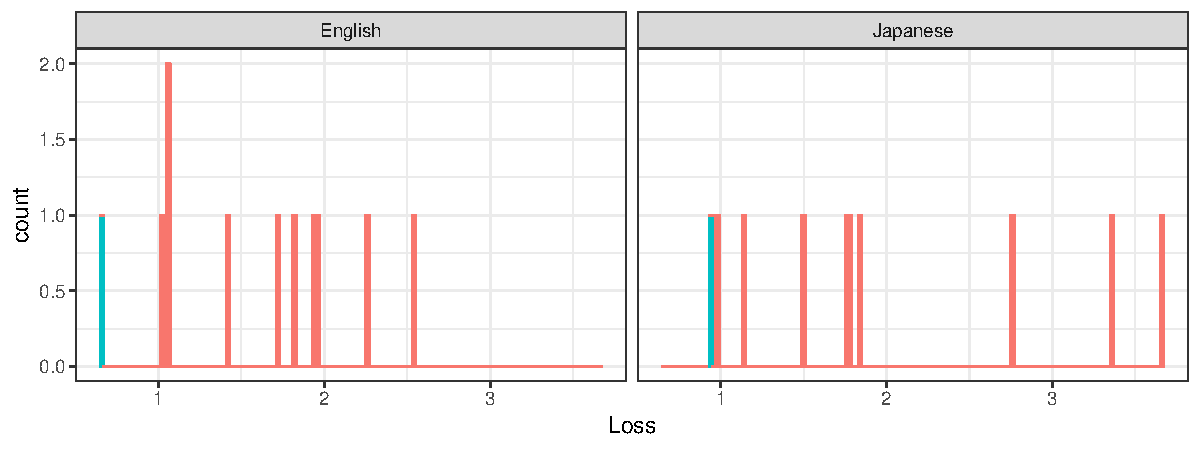
\includegraphics[scale=.7]{../results/cky/cky-parse.pdf} 
	\caption{Parsing loss $\operatorname{H}[\tree|\utterance]$ (lower is better) computed by a simple CKY parser, for random word order grammars (red) and word order grammars optimized for efficiency (blue). We report $\operatorname{H}[\tree|\utterance]$ normalized by sentence length.}
    \label{fig:cky-parser}
\end{figure}



\subsection{Distorted graph-based parsers}
\label{sec:distorted}

In this section, we address the idea that the graph-based parser might have a built-in bias toward certain kinds of orderings, and the question whether this might be responsible for our findings.
In particular, we address the idea that the graph-based parser might have a bias toward parses involving short dependencies, which we call a \key{locality bias}. 
We address this by changing the order in which the parser sees words, in such a way that the distance between words in the input is not indicative of syntactic relations.




\paragraph{Even--odd order.} A sequence of $n$ words originally ordered as $w_1 w_2 w_3 w_4 \cdots w_n$ is reordered by separating the even and odd indices: $w_2 w_4 w_6 \cdots w_{n-1} w_1 w_3 w_5 \cdots w_n$ (assuming $n$ odd). Therefore all words that are adjacent in the original order will be separated by a distance of $\approx n/2$ in the distorted order, while all words of distance 2 in the original order will become adjacent.

\paragraph{Interleaving order.} In interleaving ordering, a sequence originally ordered as $w_1 w_2 w_3 \cdots w_n$ is split in half at the middle (index $m=\ceiling{n/2}$), and the two resulting sequences are interleaved, yielding $w_1 w_m w_2 w_{m+1} w_3 w_{m+3} \cdots w_n$. Thus all words that were originally adjacent will have distance 2 in the distorted order, with the intervening word coming from a very distant part of the sentence.

\paragraph{Inwards order.} A sequence originally ordered as $w_1 w_2 w_3 \cdots w_{n-1} w_n$ is ordered from the edges of the string inwards, as $w_1 w_n w_2 w_{n-1} \cdots w_{\ceiling{n/2}}$. This corresponds to folding the string in on itself once, or equivalently, splitting the sequence in half at the middle, then interleaving the two resulting sequences after reversing the second one. The result is that the most non-local possible dependencies in the original order become the most local dependencies in the distorted order.

\paragraph{Lexicographic order.} A sequence is reordered by sorting by POS tags, and randomizing the order within each block of identical POS tags.
To each word, we then add a symbol encoding the original position in the sequence.
For instance
\begin{center}
PRON VERB PRON
\end{center}
may be reordered as
\begin{center}
PRON 1 PRON 3 VERB 2
\end{center}
or
\begin{center}
PRON 3 PRON 1 VERB 2
\end{center}
The numbers are provided to the parser as atomic symbols from a vocabulary ranging from 1 to 200; numbers greater than 200 (which may occur in extremely long sentences) are replaced by an out-of-range token.

The result is that distance between words in the input is not indicative at all of the presence of absence of syntactic relations between them.

\paragraph{Experiments}
Using English and Japanese data, we trained parsers for ten random word order grammars and for the best grammar optimized for efficiency, with the input presented in each of the distorted orderings.
Resulting parsing scores are shown in Figure~\ref{fig:distorted-parser}.
In all settings, the language optimized for efficiency achieved lower parsing loss (i.e., higher parseability) than random ordering grammars, showing that the parser's preference for optimized languages cannot be attributed to a locality bias.

\begin{figure}
    \centering
    English
    
    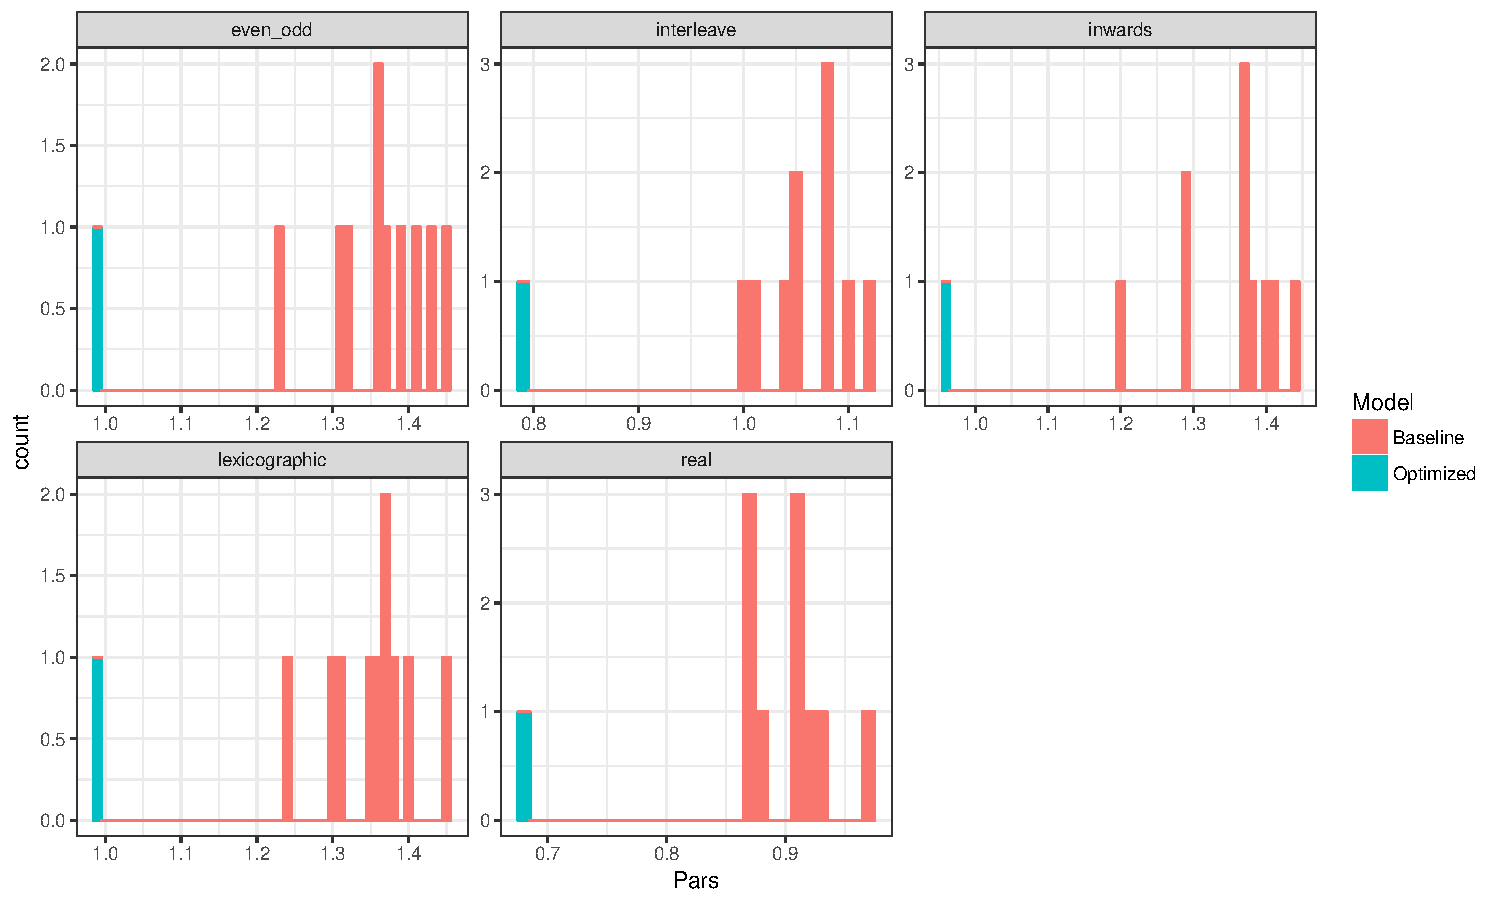
\includegraphics[scale=.5]{../results/permuted/adversarial-parse-loss-english.pdf}
    
    Japanese
    
    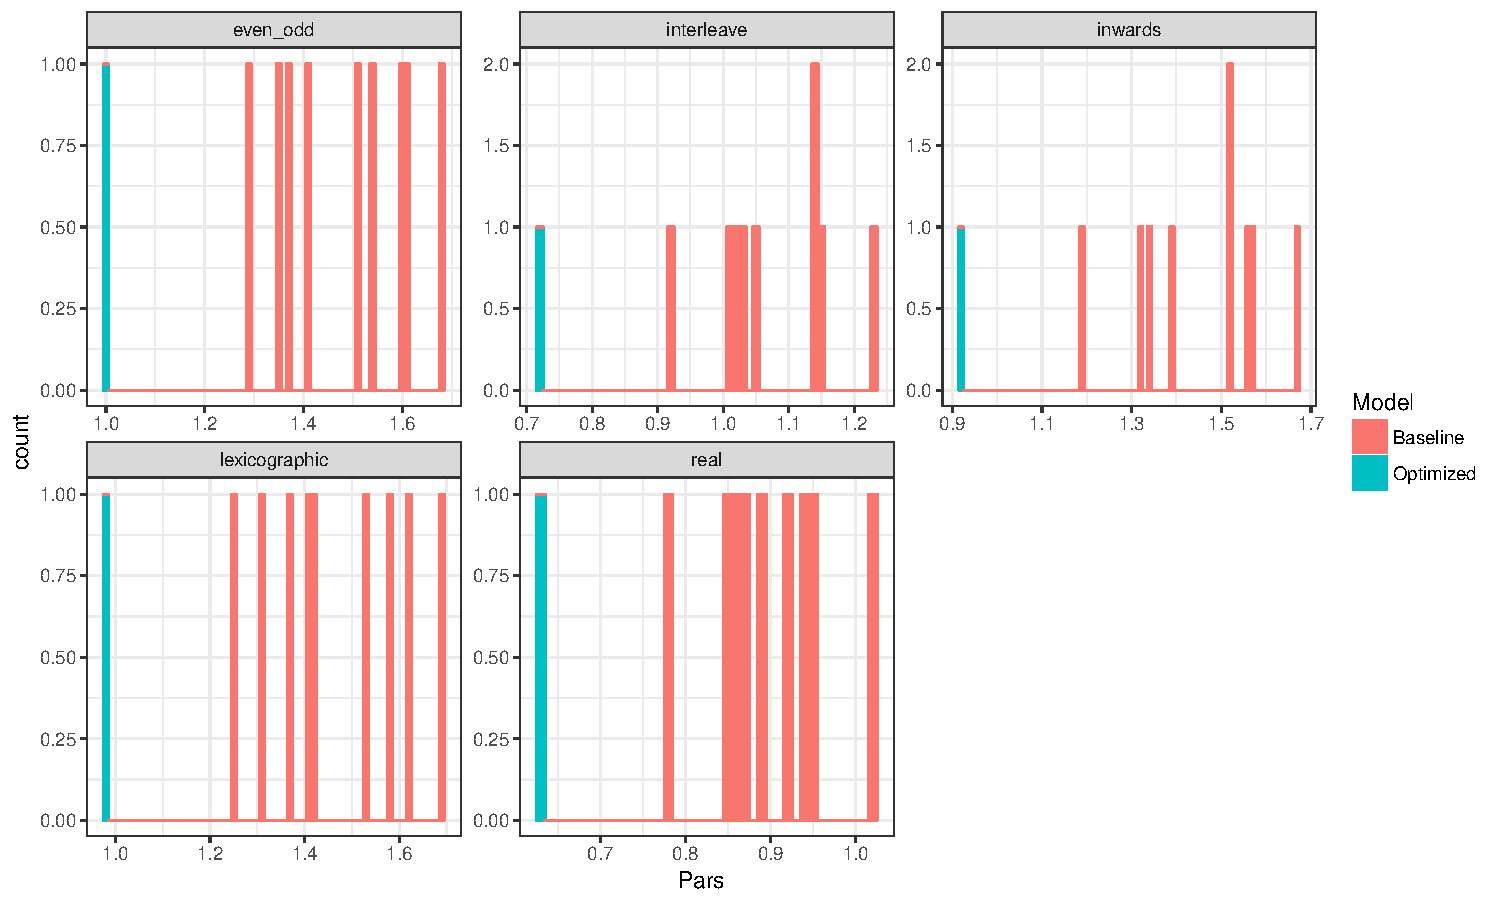
\includegraphics[scale=.5]{../results/permuted/adversarial-parse-loss-japanese.pdf}
	\caption{Parseability of baseline grammars and grammars optimized for efficiency, in English (top) and Japanese (bottom), measured by parsing loss $\operatorname{H}[\tree|\utterance]$ (lower is better), for the four distorted orderings, and the actual orderings (`real'). We report $\operatorname{H}[\tree|\utterance]$ normalized by sentence length.}
    \label{fig:distorted-parser}
\end{figure}


\subsection{$n$-gram language models}

We model predictability using LSTM language models, which are are the strongest known predictors of the surprisal effect on human processing effort~\citep{frank2011insensitivity,goodkind2018predictive}.
In previous work, such as \cite{gildea2015human}, predictability has often been measured using $n$-gram models.

Here, we show that languages optimized for LSTM predictability are also optimal for $n$-gram predictability.
Specifically, we constructed bigram models with Kneser-Ney smoothing~\cite{kneser1995improved, chen1999empirical}.
A bigram model predicts each word taking only the previous word into account.
This contrasts with LSTMs, which take the entire context into consideration.
Thus, bigram models and LSTMs stand on opposing ends of a spectrum of language models taking more and more aspects of the context into account.

We estimated language models on the training partitions, and used the validation partitions to estimate surprisal.
We conducted this for ten random and the best optimized ordering grammars on English and Japanese data.
Results (Figure~\ref{fig:bigrams}) show that languages optimized for efficiency are also optimal for a bigram language model.

\begin{figure}
    \centering
    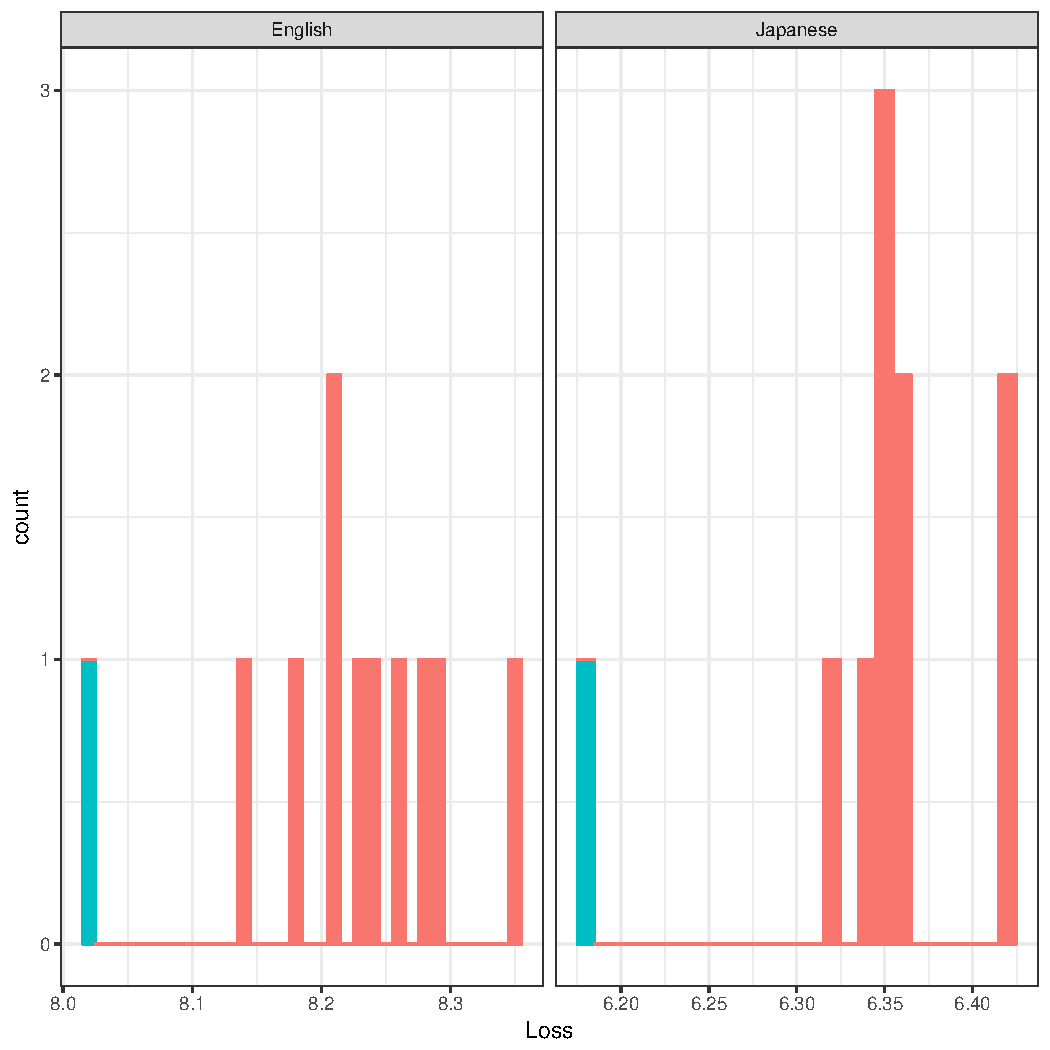
\includegraphics[scale=.6]{../results/bigrams/bigrams.pdf} 
	\caption{Surprisal (i.e., negative predictability, lower is better) computed from Bigram model, on English and Japanese data ordered according to random ordering grammars (red) and ordering grammars optimized for efficiency (blue).}
    \label{fig:bigrams}
\end{figure}



\section{Other Methods of Estimating Efficiency and Efficiency Optimization}

\subsection{Lexicalized Models}






Here we replicate Study 1 with both parsers and language models operating entirely on word forms, without POS tags.
Results are shown in Figures~\ref{fig:pareto-plane-noPOS}.
As shown in Figure~\ref{fig:byLambda-noPOS}, most real grammars have higher efficiency than most baselines across permissible values of $\lambda$.

\begin{figure}
\centering
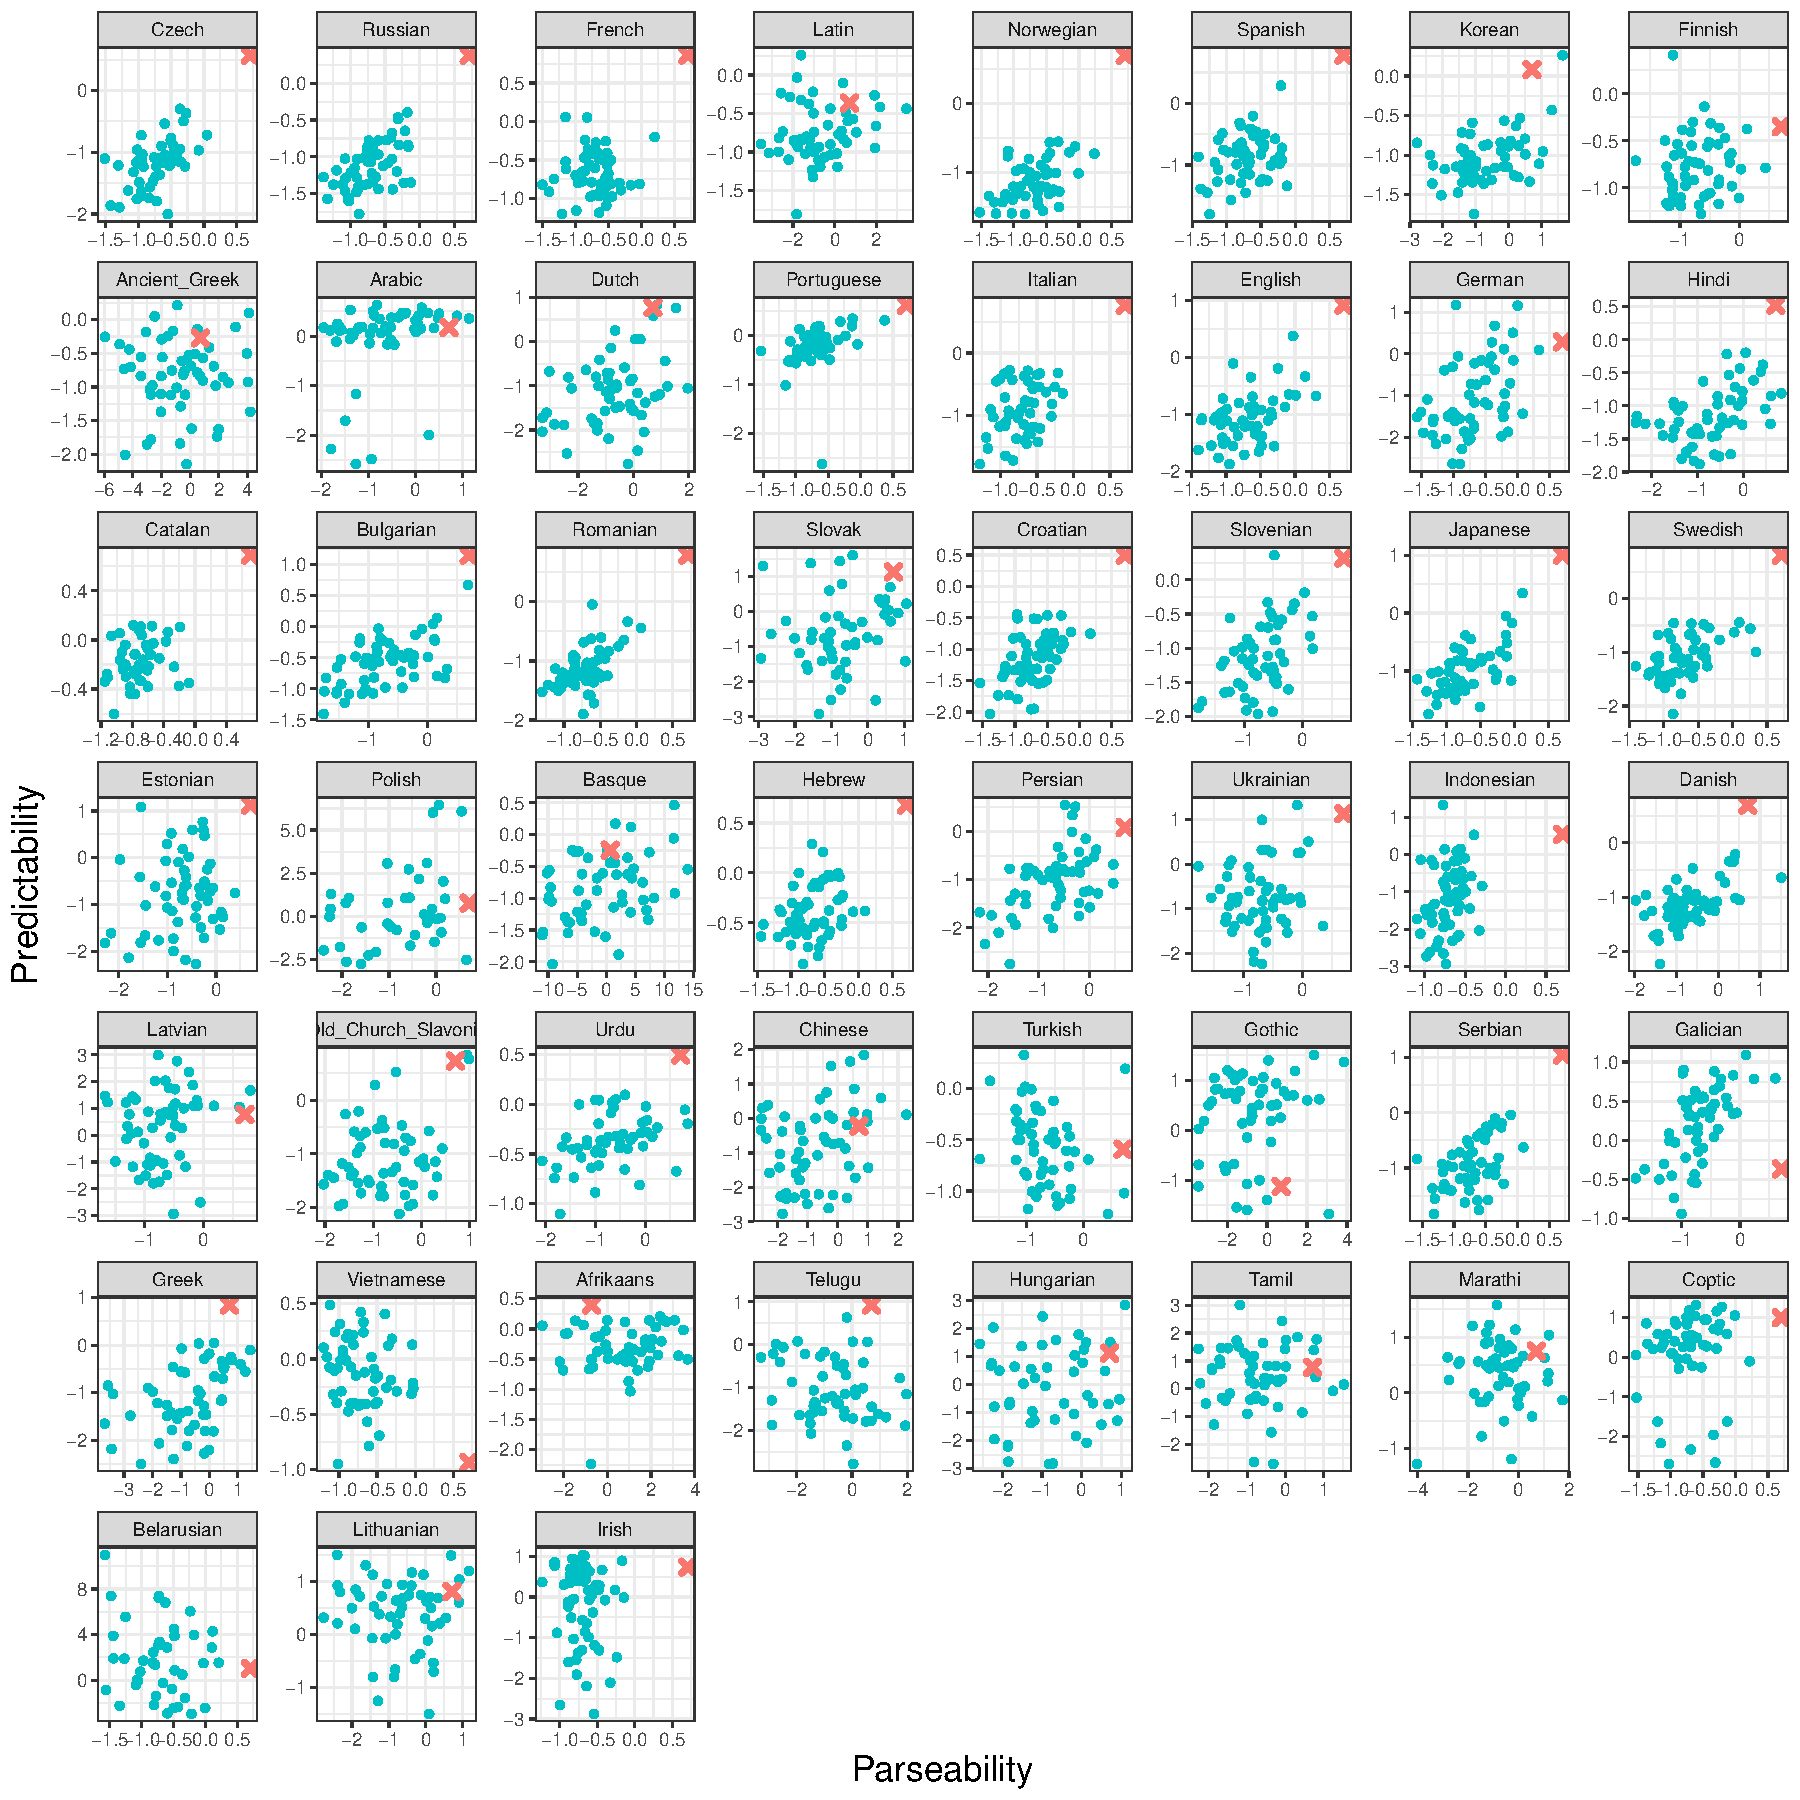
\includegraphics[width=\textwidth]{../results/plane/unlexicalized/pareto-plane-perLanguage-lexicalized.pdf}
	\caption[Predictability and Parseability]{Study 1, replication with lexicalized models: Predictability and parseability of 51 languages, for \emph{lexicalized} models, compare Figure~\ref{fig:pareto-per-lang}.}\label{fig:pareto-plane-noPOS}
\end{figure}


\begin{table}
\centering
\small{
\begin{tabular}{l||ll|lll|lll}
Language & Pred. (t) & Parse. (t) & \multicolumn{3}{c|}{Pred. (Binomial)} & \multicolumn{3}{c}{Parseab. (Binomial)} \\ 
&  $p$ & $p$ &  Est. &CI & $p$ & Est. & CI & $p$  \\ \hline \hline
Afrikaans  & \num{0.00945} & \num{0.97} & $1$ & $[0.95,1]$ & \num{<2e-16} & $0.44$ & $[0.33,1]$ & \num{0.83}\\ 
Ancient Greek  & \num{2.4e-10} & \num{1} & $0.84$ & $[0.73,1]$ & \num{2.17e-07} & $0.29$ & $[0.19,1]$ & \num{0.999}\\ 
Arabic  & \num{1} & \num{<2e-16} & $0.04$ & $[0.01,1]$ & \num{1} & $0.96$ & $[0.89,1]$ & \num{4.28e-14}\\ 
Basque  & \num{6.39e-12} & \num{1} & $0.93$ & $[0.84,1]$ & \num{1.02e-11} & $0.27$ & $[0.18,1]$ & \num{1}\\ 
Belarusian  & \num{0.0417} & \num{<2e-16} & $0.56$ & $[0.44,1]$ & \num{0.209} & $1$ & $[0.95,1]$ & \num{<2e-16}\\ 
Bulgarian  & \num{<2e-16} & \num{<2e-16} & $1$ & $[0.95,1]$ & \num{<2e-16} & $1$ & $[0.95,1]$ & \num{<2e-16}\\ 
Catalan  & \num{1.27e-05} & \num{<2e-16} & $1$ & $[0.95,1]$ & \num{<2e-16} & $1$ & $[0.95,1]$ & \num{<2e-16}\\ 
Chinese  & \num{0.000172} & \num{0.00271} & $0.66$ & $[0.54,1]$ & \num{0.0111} & $0.73$ & $[0.62,1]$ & \num{0.000343}\\ 
Coptic  & \num{4.06e-06} & \num{<2e-16} & $0.85$ & $[0.75,1]$ & \num{6.92e-08} & $1$ & $[0.95,1]$ & \num{<2e-16}\\ 
Croatian  & \num{<2e-16} & \num{<2e-16} & $1$ & $[0.95,1]$ & \num{<2e-16} & $1$ & $[0.95,1]$ & \num{<2e-16}\\ 
Czech  & \num{<2e-16} & \num{3.41e-12} & $1$ & $[0.94,1]$ & \num{2.22e-16} & $1$ & $[0.83,1]$ & \num{1.53e-05}\\ 
Danish  & \num{<2e-16} & \num{<2e-16} & $1$ & $[0.95,1]$ & \num{<2e-16} & $1$ & $[0.95,1]$ & \num{<2e-16}\\ 
Dutch  & \num{<2e-16} & \num{<2e-16} & $0.98$ & $[0.92,1]$ & \num{1.55e-15} & $0.96$ & $[0.89,1]$ & \num{4.28e-14}\\ 
English  & \num{<2e-16} & \num{<2e-16} & $1$ & $[0.95,1]$ & \num{<2e-16} & $1$ & $[0.95,1]$ & \num{<2e-16}\\ 
Estonian  & \num{<2e-16} & \num{<2e-16} & $1$ & $[0.95,1]$ & \num{<2e-16} & $1$ & $[0.95,1]$ & \num{<2e-16}\\ 
Finnish  & \num{3.92e-13} & \num{<2e-16} & $0.92$ & $[0.84,1]$ & \num{3.53e-11} & $1$ & $[0.95,1]$ & \num{<2e-16}\\ 
French  & \num{7.81e-08} & \num{<2e-16} & $1$ & $[0.95,1]$ & \num{<2e-16} & $1$ & $[0.95,1]$ & \num{<2e-16}\\ 
Galician  & \num{0.343} & \num{<2e-16} & $0.18$ & $[0.1,1]$ & \num{1} & $0.98$ & $[0.92,1]$ & \num{7.91e-16}\\ 
German  & \num{8.14e-16} & \num{<2e-16} & $0.93$ & $[0.84,1]$ & \num{5.5e-12} & $1$ & $[0.95,1]$ & \num{<2e-16}\\ 
Gothic  & \num{1} & \num{0.332} & $0.07$ & $[0.03,1]$ & \num{1} & $0.57$ & $[0.45,1]$ & \num{0.17}\\ 
Greek  & \num{<2e-16} & \num{<2e-16} & $1$ & $[0.95,1]$ & \num{<2e-16} & $1$ & $[0.95,1]$ & \num{<2e-16}\\ 
Hebrew  & \num{0.000744} & \num{<2e-16} & $1$ & $[0.95,1]$ & \num{<2e-16} & $1$ & $[0.95,1]$ & \num{<2e-16}\\ 
Hindi  & \num{<2e-16} & \num{1.32e-15} & $1$ & $[0.95,1]$ & \num{<2e-16} & $0.91$ & $[0.82,1]$ & \num{1.95e-10}\\ 
Hungarian  & \num{1.28e-07} & \num{<2e-16} & $0.79$ & $[0.68,1]$ & \num{1.12e-05} & $1$ & $[0.95,1]$ & \num{<2e-16}\\ 
Indonesian  & \num{<2e-16} & \num{<2e-16} & $0.98$ & $[0.92,1]$ & \num{1.55e-15} & $1$ & $[0.95,1]$ & \num{<2e-16}\\ 
Italian  & \num{9.09e-11} & \num{<2e-16} & $1$ & $[0.94,1]$ & \num{4.44e-16} & $1$ & $[0.94,1]$ & \num{8.88e-16}\\ 
Japanese  & \num{<2e-16} & \num{<2e-16} & $1$ & $[0.95,1]$ & \num{<2e-16} & $1$ & $[0.95,1]$ & \num{<2e-16}\\ 
Korean  & \num{<2e-16} & \num{6.52e-13} & $0.98$ & $[0.92,1]$ & \num{1.55e-15} & $0.87$ & $[0.77,1]$ & \num{1.15e-08}\\ 
Latin  & \num{4.92e-11} & \num{<2e-16} & $0.85$ & $[0.75,1]$ & \num{6.92e-08} & $0.98$ & $[0.92,1]$ & \num{3.05e-15}\\ 
Latvian  & \num{0.0107} & \num{<2e-16} & $0.52$ & $[0.4,1]$ & \num{0.446} & $1$ & $[0.95,1]$ & \num{<2e-16}\\ 
Lithuanian  & \num{5.64e-05} & \num{1.4e-12} & $0.75$ & $[0.64,1]$ & \num{0.000134} & $0.91$ & $[0.81,1]$ & \num{3.54e-10}\\ 
Marathi  & \num{1.07e-05} & \num{8.79e-09} & $0.74$ & $[0.62,1]$ & \num{0.000268} & $0.78$ & $[0.66,1]$ & \num{2.6e-05}\\ 
Norwegian  & \num{<2e-16} & \num{<2e-16} & $1$ & $[0.94,1]$ & \num{2.22e-16} & $1$ & $[0.94,1]$ & \num{2.22e-16}\\ 
Old Church Slavonic  & \num{<2e-16} & \num{4.93e-13} & $0.96$ & $[0.89,1]$ & \num{2.22e-14} & $0.89$ & $[0.8,1]$ & \num{5.09e-10}\\ 
Persian  & \num{<2e-16} & \num{<2e-16} & $0.94$ & $[0.86,1]$ & \num{2.76e-12} & $1$ & $[0.95,1]$ & \num{<2e-16}\\ 
Polish  & \num{1.4e-05} & \num{<2e-16} & $0.73$ & $[0.61,1]$ & \num{0.000508} & $1$ & $[0.95,1]$ & \num{<2e-16}\\ 
Portuguese  & \num{0.0269} & \num{<2e-16} & $1$ & $[0.95,1]$ & \num{<2e-16} & $1$ & $[0.95,1]$ & \num{<2e-16}\\ 
Romanian  & \num{<2e-16} & \num{<2e-16} & $1$ & $[0.95,1]$ & \num{<2e-16} & $1$ & $[0.95,1]$ & \num{<2e-16}\\ 
Russian  & \num{<2e-16} & \num{<2e-16} & $1$ & $[0.95,1]$ & \num{<2e-16} & $1$ & $[0.95,1]$ & \num{<2e-16}\\ 
Serbian  & \num{<2e-16} & \num{<2e-16} & $1$ & $[0.95,1]$ & \num{<2e-16} & $1$ & $[0.95,1]$ & \num{<2e-16}\\ 
Slovak  & \num{<2e-16} & \num{<2e-16} & $0.93$ & $[0.84,1]$ & \num{1.9e-11} & $1$ & $[0.95,1]$ & \num{<2e-16}\\ 
Slovenian  & \num{<2e-16} & \num{<2e-16} & $0.98$ & $[0.91,1]$ & \num{1.18e-14} & $1$ & $[0.95,1]$ & \num{<2e-16}\\ 
Spanish  & \num{1.87e-12} & \num{<2e-16} & $1$ & $[0.95,1]$ & \num{<2e-16} & $1$ & $[0.95,1]$ & \num{<2e-16}\\ 
Swedish  & \num{<2e-16} & \num{<2e-16} & $1$ & $[0.95,1]$ & \num{<2e-16} & $1$ & $[0.95,1]$ & \num{<2e-16}\\ 
Tamil  & \num{0.0113} & \num{0.000641} & $0.58$ & $[0.46,1]$ & \num{0.136} & $0.7$ & $[0.59,1]$ & \num{0.00192}\\ 
Telugu  & \num{<2e-16} & \num{1.95e-15} & $1$ & $[0.95,1]$ & \num{<2e-16} & $0.93$ & $[0.84,1]$ & \num{1.9e-11}\\ 
Turkish  & \num{0.711} & \num{<2e-16} & $0.47$ & $[0.35,1]$ & \num{0.708} & $0.96$ & $[0.89,1]$ & \num{1.59e-13}\\ 
Ukrainian  & \num{<2e-16} & \num{<2e-16} & $0.98$ & $[0.92,1]$ & \num{1.55e-15} & $1$ & $[0.95,1]$ & \num{<2e-16}\\ 
Urdu  & \num{0.0205} & \num{1.63e-14} & $1$ & $[0.94,1]$ & \num{4.44e-16} & $0.88$ & $[0.78,1]$ & \num{5.16e-09}\\ 
Vietnamese  & \num{1} & \num{<2e-16} & $0.02$ & $[0,1]$ & \num{1} & $1$ & $[0.95,1]$ & \num{<2e-16}\\ 

\end{tabular}
}
	\caption{Study 1, replication with lexicalized models: Per-language results in Study 1, with \emph{lexicalized} parsers and word-level-only language models. Compare Table~\ref{fig:pareto-per-lang-stats}}\label{tab:pareto-plane-noPOS}
\end{table}


\begin{figure}
	\centering
	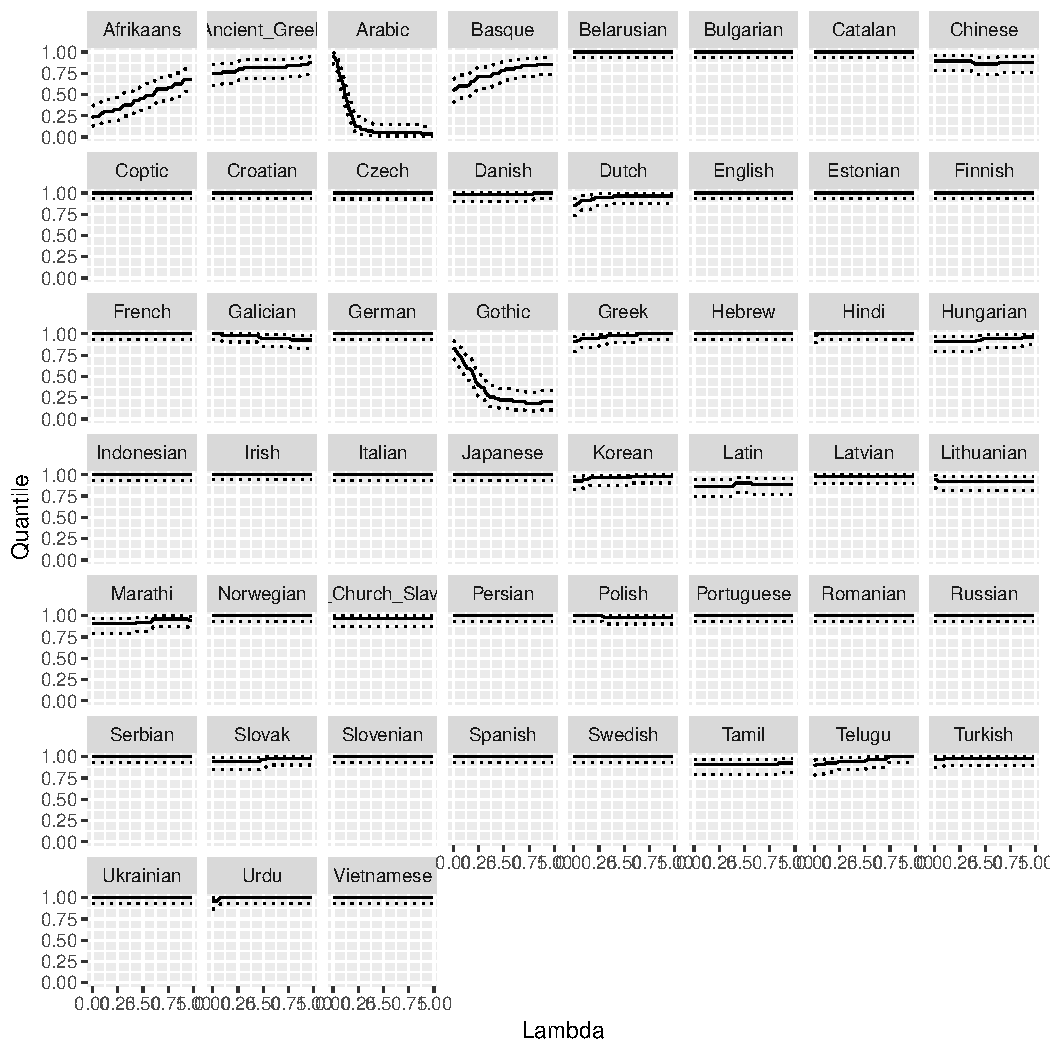
\includegraphics[width=\textwidth]{../results/plane/unlexicalized/analyze_pareto_optimality/figures/quantileByLambda-mle.pdf}
	\caption{Study 1, replication with lexicalized models: Optimality by $\lambda$ (lexicalized models).}\label{fig:byLambda-noPOS}
\end{figure}


\subsection{Original UD Format}

We replicate the comparison between real and random grammars in Study 1.

\begin{figure}
\centering
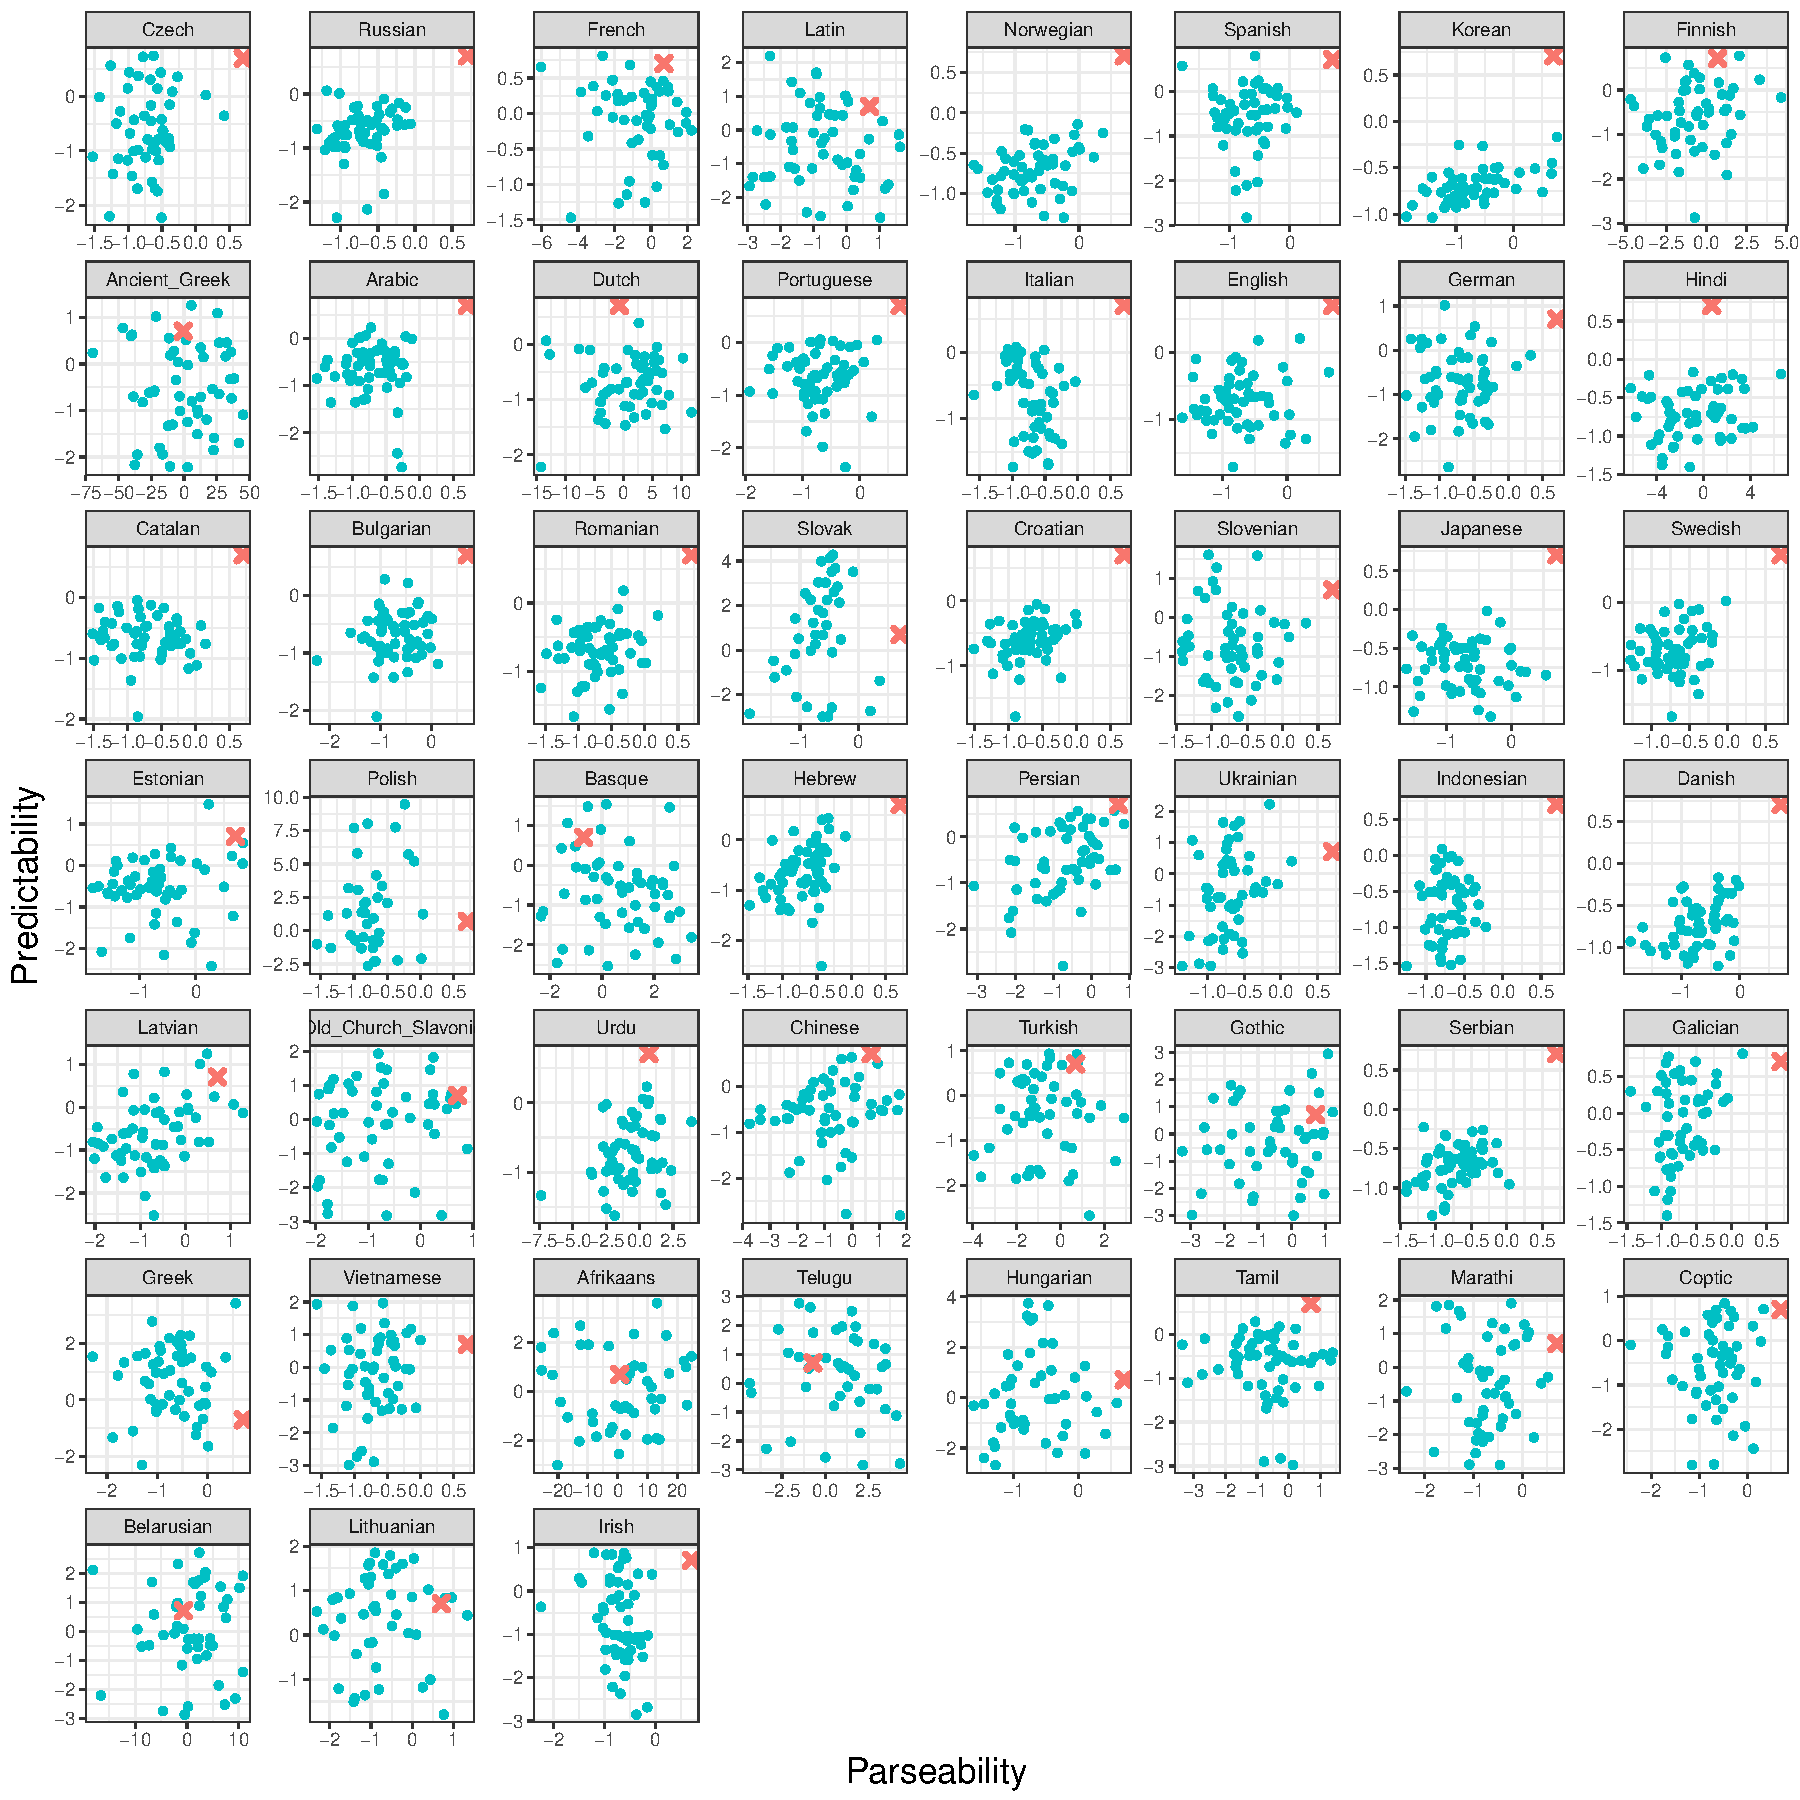
\includegraphics[width=\textwidth]{../results/plane/pureUD/pareto-plane-perLanguage-pureUD-mle.pdf}
	\caption[Predictability and Parseability]{Study 1, replication with the original UD format models: Predictability and parseability of 51 languages, for \emph{lexicalized} models, compare Figure~\ref{fig:pareto-per-lang-pureUD}.}
\end{figure}




\begin{figure}
	\centering
	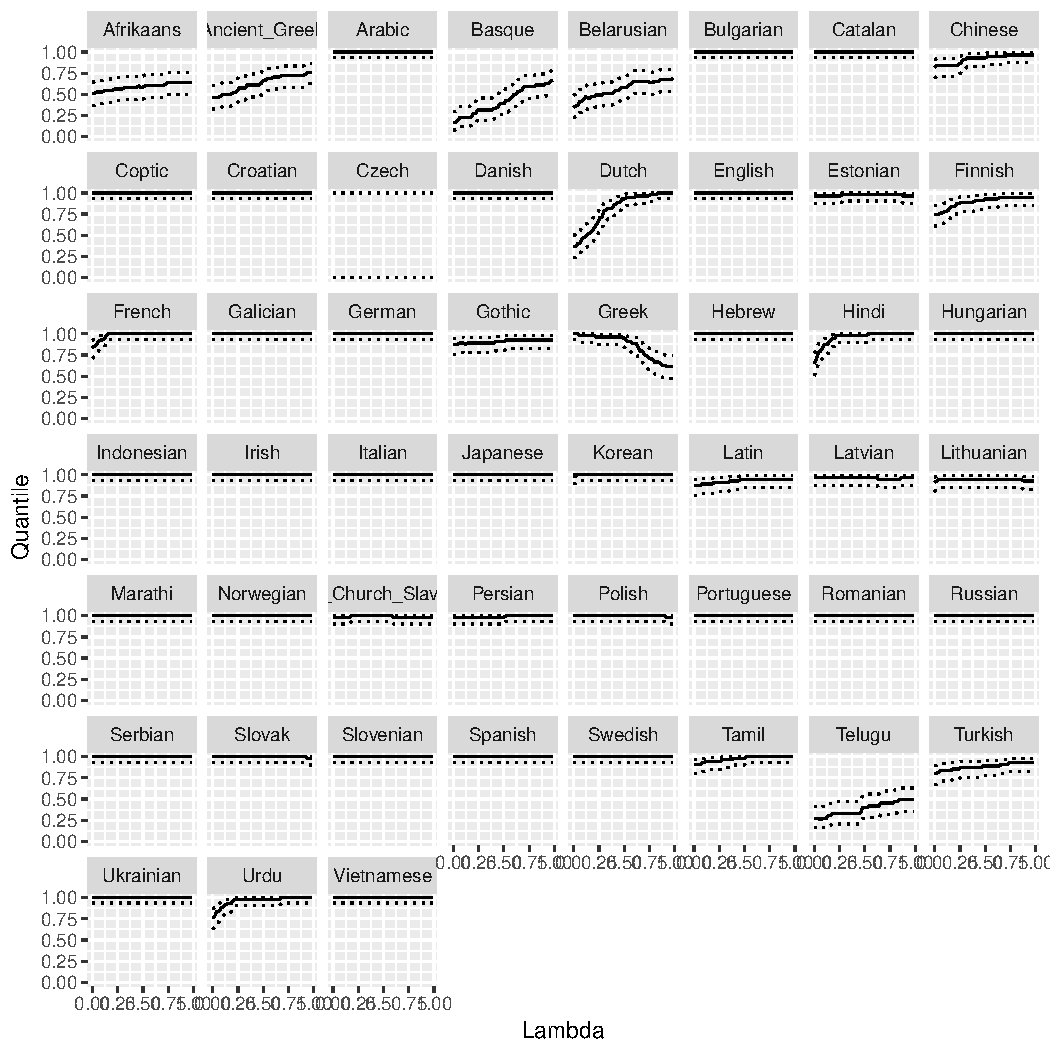
\includegraphics[width=\textwidth]{../results/plane/pureUD/analyze_pareto_optimality/figures/quantileByLambda-mle.pdf}
	\caption{Study 1, replication with original UD format: Optimality by $\lambda$ (lexicalized models).}
\end{figure}




\subsection{Nondeterministic Baseline Grammars}

In Study 1, we considered deterministic ordering grammars, even though real languages have some degree of word order freedom.
Here, we show that deterministic baseline grammars provide conservative baselines: They have higher efficiency than baseline grammars with word order freedom comparable to real languages.


In order to obtain baselines whose freedom is comparable to that of real languages, we constructed baselines that have the same Branching Direction Entropy \cite{futrell2015quantifying}:
For every one of the 37 syntactic relations, we chose $a_\tau$ the direction entropy to be the same as observed in the actual orderings found in the UD corpus.
We kept the relative ordering of siblings on one side deterministic, i.e., we considered the limit where the values $b_\tau$ for different $\tau$ are far apart.

Results are shown in Figure~\ref{fig:nondeterministic-english}.
For every one of the baseline grammars, we show both its deterministic and its nondeterministic version.
Nondeterministic grammars are strongly less efficient than deterministic grammars, showing that deterministic grammars constitute stronger baselines.

\begin{figure}
	\centering
	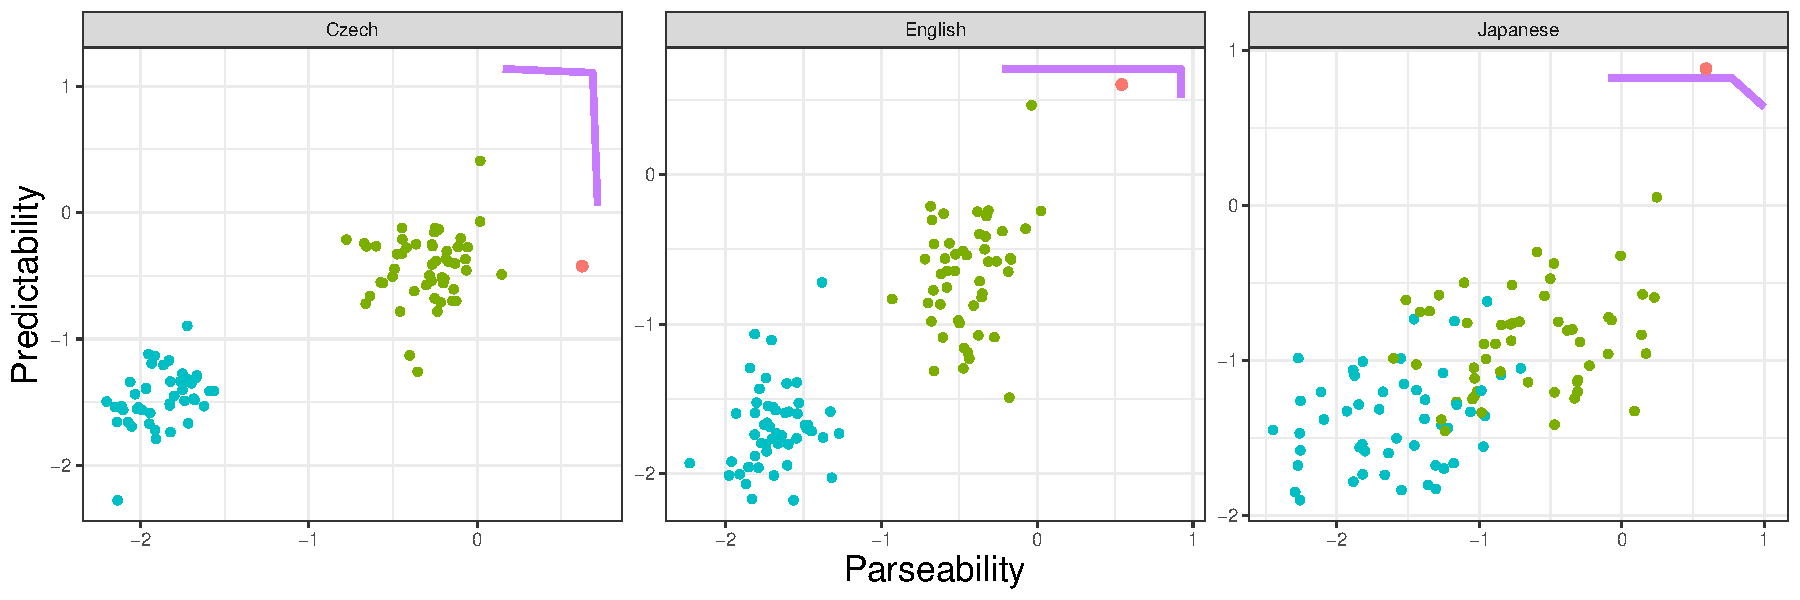
\includegraphics[width=0.4\textwidth]{../results/plane/nondeterministic/pareto-plane-perLanguage-nondeterministic-mle.pdf}
	\caption{Parseability and predictability, including nondeterministic versions of the 50 baseline grammars.}\label{fig:nondeterministic-english}
\end{figure}






\section{Effects of data sparsity}

Here, we investigate whether the difference between real and baseline grammars is affected by the size of available datasets.
We are addressing the following confound: It is conceivable that with enough data, our neural network language models and parsers would do equally well on real grammars and baseline grammars.
If the difference between random and real grammars is due to data sparsity in this way, then we expect that the difference will decrease as the amount of training data is increased.
If, on the other hand, there is an inherent difference in efficiency between random and real grammars, we expect that the difference will persist as training data is increased.

We considered Czech, the UD language with the largest amount of available treebank data (approx. 2.2 million words), up to $\approx$ 300 times more data than is available for some other UD languages.
We considered both a random ordering grammar, and the best ordering grammar optimized for parseabaility.
For both of these ordering grammars, we trained the parser on successively larger portions of the training data (0.1 \%, 1 \%, 5\%, 10\%, 20 \%, ..., 90 \%, 100 \%) and recorded parsing accuracy.
Furthermore, for the random grammar, we varied the number of neurons in the BiLSTM (200, 400, 800) to test whether results depend on the capacity of the network.


The resulting curves are shown in Figure~\ref{fig:learning-czech}.
%A gap in parsing accuracy of about 0.07-0.1 appears already at 0.01 \% of the training data (2000 words), and persists for larger amounts of training data.
A gap in parsing loss of about 0.2 nats appears already at 0.01 \% of the training data (2000 words), and persists for larger amounts of training data.
This shows that the observed efficiency differences between grammars cannot be attributed to data sparsity. 

\begin{figure}[ht]
    \centering
%    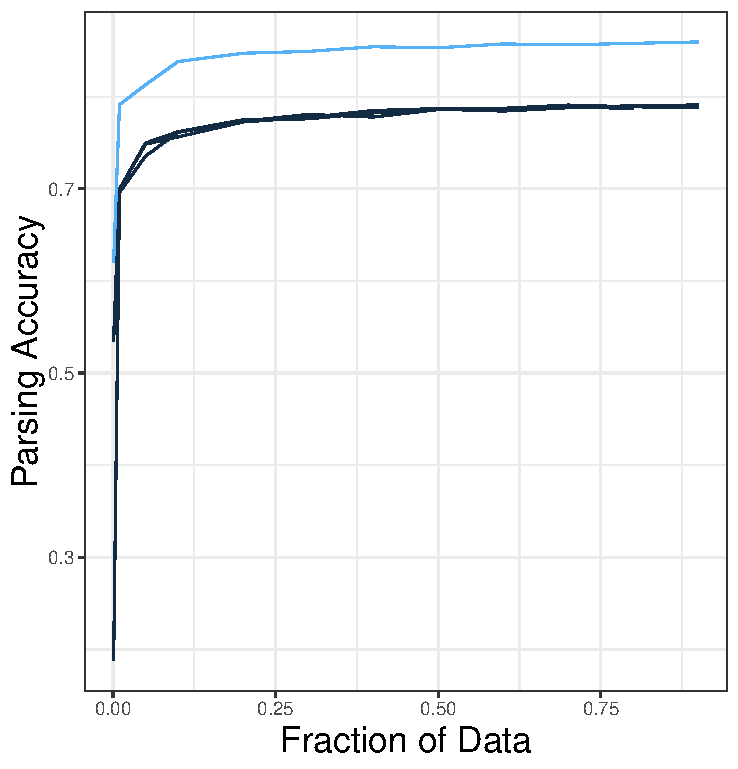
\includegraphics[scale=.4]{../results/learning-curves/figures/learning-parser-czech.pdf} 
    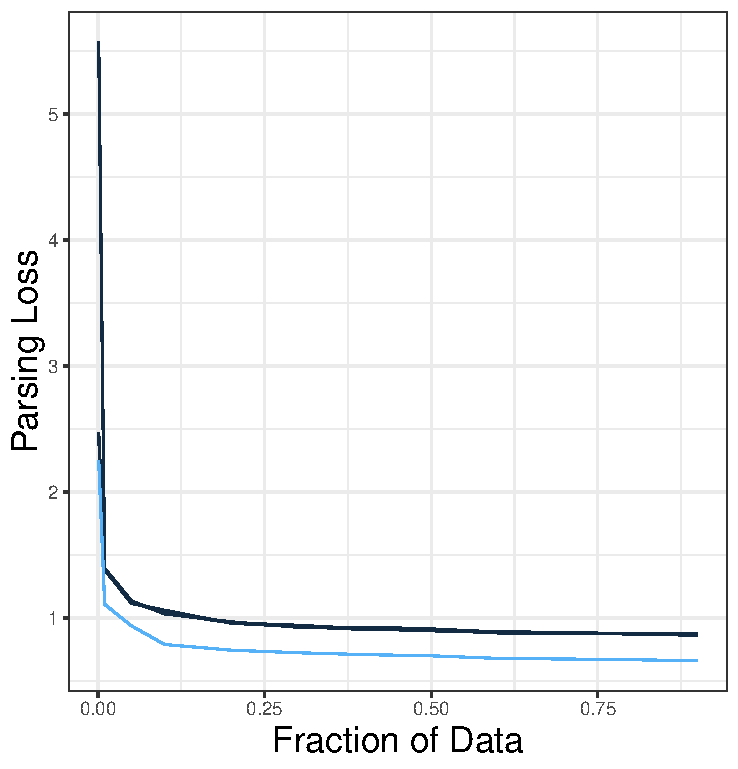
\includegraphics[scale=.4]{../results/learning-curves/figures/learning-parser-czech-logloss.pdf} 

	\caption{Parsing loss ($\operatorname{H}[\tree|\utterance]$, normalized by sentence length) for optimized (light blue) and random (black) ordering grammar on Czech data, as a function of the fraction of total training data provided.}
    \label{fig:learning-czech}
\end{figure}







\section{Languages and Corpus Sizes}
In Table~\ref{tab:langs-iso-sizes}, we list the 51 languages with ISO codes and families, with the size of the available data per language.
We included all UD 2.1 languages for which a training partition was available.

%Among UD 2.1 corpora, three treebanks require a special license (Arabic-NYUAD, French-FTB).
%For a few UD corpora, only the syntactic annotation is freely available, while the individual words require a license.
%For the lexicalized experiment, we had access to the individual words for 

\begin{table}[ht]
\small{
\begin{tabular}{lllllll}
Language & ISO Code & Family & Sentences (train/held-out) & Words (train/held-out) \\ \hline
Afrikaans & afr & Germanic & 1315/194 & 30765/4808   \\
Ancient Greek & grc & Greek & 26322/2156 & 323993/33468   \\
Arabic & arb & Semitic & 21864/2895 & 737410/93666   \\
Basque & eus & Basque & 5396/1798 & 61040/20122   \\
Belarusian & bel & Slavic & 260/65 & 4328/1274   \\
Bulgarian & bul & Slavic & 8907/1115 & 106813/13822   \\
Catalan & cat & Romance & 13123/1709 & 375524/50954   \\
Chinese & cmn & Sino-Tibetan & 3997/500 & 85013/10899   \\
Coptic & cop & Egyptian & 364/41 & 8818/871   \\
Croatian & hrv & Slavic & 7689/600 & 148560/12922   \\
Czech & ces & Slavic & 102993/11311 & 1547431/163578   \\
Danish & dan & Germanic & 4383/564 & 69273/8952   \\
Dutch & nld & Germanic & 18310/1518 & 234859/19115   \\
English & eng & Germanic & 17062/3070 & 263328/39537   \\
Estonian & est & Finnic & 6959/855 & 69754/8709   \\
Finnish & fin & Finnic & 27198/3239 & 248283/29204   \\
French & fra & Romance & 32347/3232 & 780289/77416   \\
Galician & glg & Romance & 2472/1260 & 76208/36450   \\
German & deu & Germanic & 13814/799 & 229204/10727   \\
Gothic & got & Germanic & 3387/985 & 35024/10114   \\
Greek & ell & Greek & 1662/403 & 38139/9404   \\
Hebrew & heb & Semitic & 5241/484 & 122122/10050   \\
Hindi & hin & Indic & 13304/1659 & 262389/32850   \\
Hungarian & hun & Ugric & 910/441 & 17282/9974   \\
Indonesian & ind & Malayo-Sumbawan & 4477/559 & 82963/10676   \\
Irish & gle & Celtic & 121/445 & 2864/9554   \\
Italian & ita & Romance & 17427/1070 & 329477/18790   \\
Japanese & jpn & Japanese & 7164/511 & 145240/10404   \\
Korean & kor & Korean & 27410/3016 & 312830/32849   \\
Latin & lat & Latin & 30598/2568 & 387236/29858   \\
Latvian & lav & Baltic & 4124/989 & 51562/10773   \\
Lithuanian & lit & Baltic & 153/55 & 2536/883   \\
Marathi & mar & Indic & 373/46 & 2447/342   \\
Norwegian & nob & Germanic & 29870/4639 & 432741/62802   \\
Old Church Slavonic & chu & Slavic & 4123/1073 & 37432/10100   \\
Persian & pes & Iranian & 4798/599 & 110345/14474   \\
Polish & pol & Slavic & 6100/1027 & 52445/8613   \\
Portuguese & por & Romance & 17995/1770 & 401487/37388   \\
Romanian & ron & Romance & 8664/752 & 170551/14898   \\
Russian & rus & Slavic & 52664/7163 & 773678/105285   \\
Serbian & srp & Slavic & 2935/465 & 57581/8825   \\
Slovak & slk & Slavic & 8483/1060 & 65044/10648   \\
Slovenian & slv & Slavic & 7532/1817 & 106904/22083   \\
Spanish & spa & Romance & 28492/3054 & 731920/79171   \\
Swedish & swe & Germanic & 7041/1416 & 102400/23585   \\
Tamil & tam & Southern Dravidian & 400/80 & 5664/1118   \\
Telugu & tel & South-Central Dravidian & 1051/131 & 3926/519   \\
Turkish & tur & Southwestern Turkic & 3685/975 & 31271/8203   \\
Ukrainian & ukr & Slavic & 4506/577 & 61011/8384   \\
Urdu & urd & Indic & 4043/552 & 103152/13888   \\
Vietnamese & vie & Viet-Muong & 1400/800 & 17325/9873   \\

\end{tabular}
}
\caption{Languages with ISO codes, families (according to \url{https://universaldependencies.org/}), and the number of available sentences and words.}\label{tab:langs-iso-sizes}
\end{table}



\section{Dependency Length Minimization}\label{sec:DLM}



Prior work has suggested \emph{Dependency Length Minimization} (DLM) as a characteristic of efficient word order~\cite{futrell2015largescale,ferrericancho2004euclidean,liu2017dependency,temperley2018minimizing}.
This is the idea that word order minimizes the average distance between syntactically related words.
It is known that human languages reduce dependency length compared to random baselines~\cite{liu2010dependency,futrell2015largescale,liu2017dependency,temperley2018minimizing}.
Prior work has suggested principles akin to DLM as approximating efficiency optimization of grammars~\cite{hawkins1994performance,hawkins2004efficiency,futrell2017memory, futrell2017generalizing}.
It is a heuristic formalization of the idea that long dependencies should create high memory requirements in parsing and prediction~\cite{hawkins1994performance,gibson1998linguistic,gibson2000dependency, futrell2017memory}.
Indeed, \cite{futrell2017memory} argues specifically that it emerges from efficiency optimization.
%[TODO also cite rijkhof, ferrer i cancho]

Dependency length is typically quantified as the average distance between all pairs of syntactically related words, measured by the number of intervening words~\cite{futrell2015largescale}.
Dependency length quantified in this manner is a heuristic measure of complexity:
The actual empirically-measured processing complexity induced by long dependencies is not a linear function of length and depends crucially on the types of dependencies involved \cite{demberg2008data} and the specific elements intervening between the head and dependent \cite{gibson1998linguistic,gibson2000dependency,lewis2005activationbased}.

We asked whether efficiency optimization predicts dependency length minimization effects.
We first computed dependency length for grammars optimized for efficiency.
We found that 100\% of grammars optimized for efficiency reduce average dependency length compared to baseline grammars ($p < 0.05$, by one-sided $t$-test). 
This suggests that the reduction of dependency length observed in natural language is indeed predicted by efficiency maximization, confirming theoretical arguments made in prior work~\cite{hawkins1994performance,hawkins2004efficiency,futrell2017memory, futrell2017generalizing}.
Next, we constructed grammars that minimize average dependency length, using the same gradient descent method as we used for efficiency optimization (Section~\ref{sec:optim-eff}).
We expect that such grammars should have shorter dependency length than the real grammars, or grammars optimized for efficiency.
In Figure~\ref{fig:dlm-avg}, we plot the mean dependency length for optimized, real, and baseline orderings.
We find that optimizing grammars for efficiency reduces dependency length to a similar degree as found in the actual orderings in the corpora, almost up to the limit given by directly optimizing for dependency length. %[TODO acknowledge  Ferrer i Cancho R, Liu H (2014) The risks of mixing dependency lengths from se-quences of different length.Glottotheory5(2):143–155.]
We also plot more detailed results for four languages in Figure~\ref{fig:dlm-4langs}, plotting dependency length as a function of sentence length as reported in prior work \cite{futrell2015largescale}.
Optiziming grammars for efficiency produces dependency lengths similar to those found in the actual orderings.

\begin{figure}[ht]
    \centering
     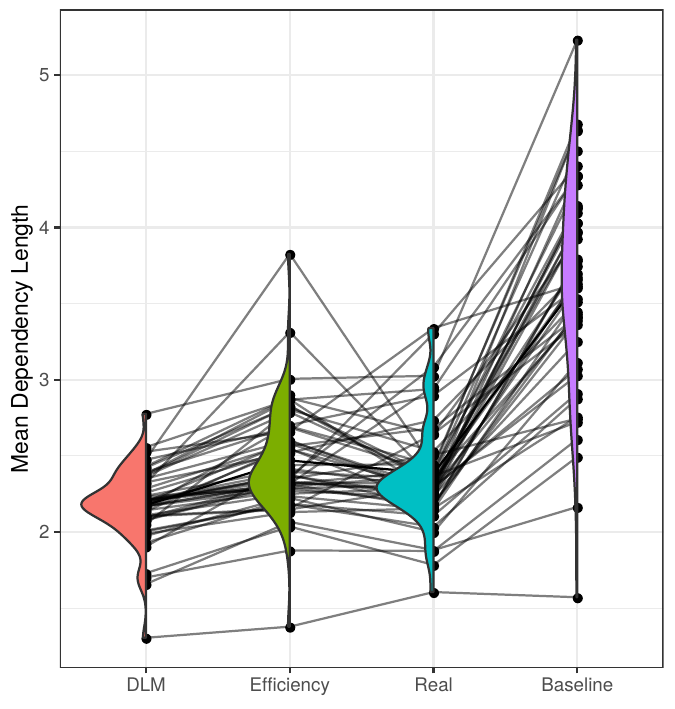
\includegraphics[width=0.5\textwidth]{depl-violin-all-1.png} 
        \caption{Average dependency length for grammars optimized to minimize dependency length (DLM, left), optimized for efficiency (second), the real orderings found in corpora (third), and random baseline grammars (right). The lines connect the mean points for each of the 51 languages in our sample.}
    \label{fig:dlm-avg}
\end{figure}

\begin{figure}[ht]
    \centering
	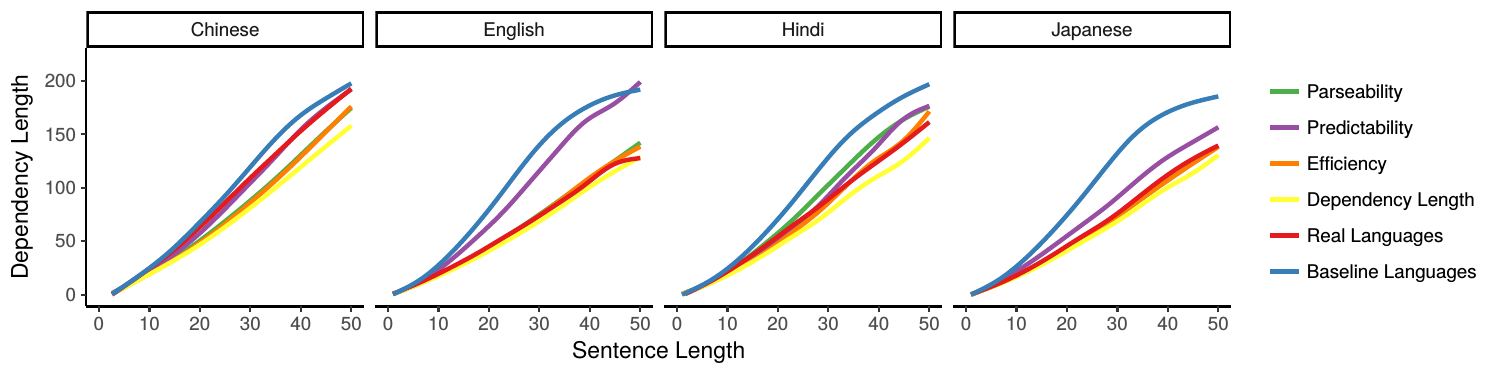
\includegraphics[width=0.9\textwidth]{depLength-facet-1.png} 
        \caption{Total dependency length as a function of sentence length, for four diverse languages. We show results for optimized grammars (parseability, predictability, efficiency), for grammars specifically optimized to minimize dependency length, of the actual real orderings, and of the baseline grammars.}
    \label{fig:dlm-4langs}
\end{figure}


Next, we examined the word order properties of grammars optimized for DLM.
In Table~\ref{tab:all-predictions-1b}, we report the posterior prevalence of word order correlations in grammars optimized for DLM; our results show that optimizing for DLM makes predictions similar to efficiency optimization.
We find that these grammars also exhibit the eight correlations, similar to grammars directly optimized for efficiency.
This is itself a novel result, suggesting that it is in part through favoring short dependencies that efficiency predicts word order universals, an idea that has been proposed in prior theoretical studies, though never tested computationally on large-scale text data \citep{kuno1974position,rijkhoff1986word,frazier1985syntactic,rijkhoff1990explaining,hawkins1994performance, hawkins2004efficiency}.
On other correlations, predictions of DLM also resemble those of efficiency optimization.
However, it predicts strong correlations with \textit{amod} (adjectival modifiers) and \textit{nummod} (numeral modifiers) (see bottom of Table~\ref{tab:all-predictions-1b}), which are not borne out typologically.
In these cases, efficiency optimization predicts prevalences closer to 50\%, in line with typological data.


\begin{table}[ht] 
	\begin{center}	
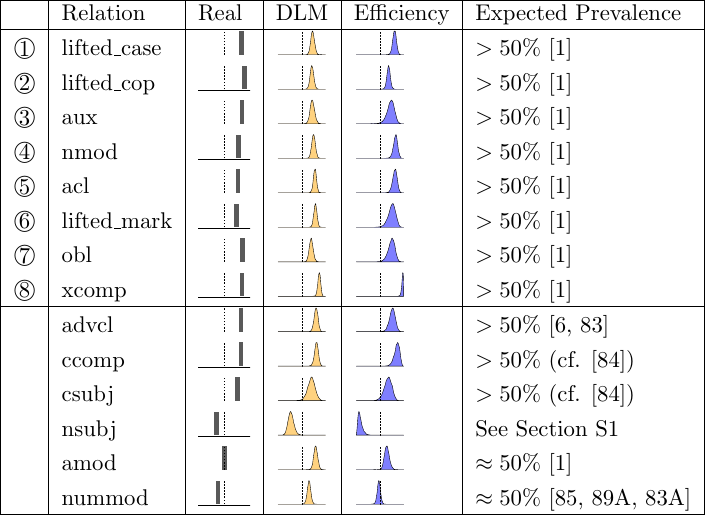
\includegraphics[width=0.7\textwidth]{si-table-perrel-1b-1.png}
\end{center}
\caption{Predictions on UD relations with predictions from the typological literature (compare Table~\ref{tab:all-predictions-1}), for languages optimized for Efficiency and Dependency Length Minimization.
}
\label{tab:all-predictions-1b}
\end{table}

In conclusion, these results suggest that the phenomenon of dependency length minimization is a by-product of efficiency optimization, providing support to theoretical arguments from the linguistic literature~\cite{hawkins1994performance,futrell2017memory, futrell2017generalizing}.
Furthermore, optimizing for dependency length correctly predicts a range of word order facts, though it appears to \emph{overpredict} correlations when compared to direct optimization for communicative efficiency.






\section{Simulation for Parseability and Correlating Orders}

%VP -> V
%VP -> VP[head] VP[xcomp]
%VP -> VP[head] NP[obj]
%
%NP -> N
%NP -> NP[head] VP[acl]

When we optimize grammars for efficiency, we find that the optimized grammars exhibit dependency length minimization and the Greenbergian word order correlations. To some extent, this result is surprising, because previous functional explanations for DLM (and the Greenbergian correlations, which are predicted by DLM) have been based on the idea of limitations in working memory, and yet our models do not instantiate any explicit working memory pressures. Nor is it the case that our parsers have implicit locality biases, as demonstrated by the experiments in Section~\ref{sec:distorted} above. Our results therefore suggest that DLM and word order correlations might arise purely because they enable tree structures to be better recovered from trees, and/or they make sequences more predictable. 

Here we perform some simulation studies to bolster the argument that DLM and word order correlations can enhance the recoverability of tree structures in a generic sense, without any appeal to memory limitations. To do so, we experiment with toy grammars that can be defined to either (1) exhibit word order correlations or (2) not, and we test whether the grammars of type (1) are more or less parseable than the grammars of type (2). We measure parseability using a CYK PCFG parser, thus removing any potential confounds arising from the neural network parsing model.

Our toy grammar consists of the following head-outward generative model.
Verbs generate verb dependents (\emph{xcomp}) and noun dependents (\emph{obj}), independently.
The overall number $N$ of dependents is $NB(1, p_\text{branching})$, the number of \emph{obj} dependents is $Binom(p_{obj}, N)$.
Nouns can generate verb dependents (\emph{acl}), of number $NB(1, p_\text{acl})$.

Trees are linearized using one of two grammars: One (`Correlating') places \emph{obj}, \emph{xcomp}, and \emph{acl} dependents on the same side of the head, and (in accordance with crosslinguistic tendencies) places the \emph{obj} dependents closer to the head than \emph{xcomp} dependents.
The other grammar (`Anti-Correlating') places \emph{xcomp} and \emph{acl} dependents opposite to \emph{obj} dependents.

An example is provided in Figure~\ref{fig:sent-dep}.
We show how the two grammars linearize the same syntactic dependency structure:
The correlating grammar (left) linearizes the three relation types towards the right of the head; the anti-correlating one places \emph{obj} dependencies on the left and the other dependencies on the right.
This example provides some intuitive idea of why the correlating grammar might lead to improved parseability:
Note that the red token labeled `N' occupies the same structural position in both versions.
In the anti-correlating version (right), when given only the token sequence, without the syntactic structure, this word could a priori be an \emph{obj} dependent of any of the three verbs occurring to its right.
In the correlating version (left), this `N' token can only possibly be a dependent of the verb occurring to its left.

\begin{figure}[ht]
    \centering
{
\centering{
\begin{dependency}[theme = simple]
   \begin{deptext}[column sep=1em]
	   V \& \textcolor{red}{N} \& V \& N \& V  \\
   \end{deptext}
   \depedge{1}{2}{obj}
   \depedge{2}{3}{acl}
   \depedge{3}{4}{obj}
   \depedge{1}{5}{xcomp}
\end{dependency}
\begin{dependency}[theme = simple]
   \begin{deptext}[column sep=1em]
	   \textcolor{red}{N} \& N \& V \&  V \&  V   \\
   \end{deptext}
   \depedge{4}{1}{obj}
   \depedge{1}{3}{acl}
   \depedge{3}{2}{obj}
   \depedge{4}{5}{xcomp}
\end{dependency}

}
}
	\caption{Linearizations of a syntactic dependency structure, under a correlating grammar (left) and an anti-correlating grammar (right).}
	\label{fig:sent-dep}
\end{figure}


In order to test this intuition on the level of the entire tree distribution, we formulated this model as a binary-branching PCFG, and used a CKY parser to estimate $I[\mathcal{T}, \mathcal{U}]$ from 10,000 random sample sentences.

We computed this for different settings of $p_\text{branching} \in [0, 0.5]$ and $p_{obj} \in [0,1]$, at $p_\text{acl} \in \{0, 0.3\}$.\footnote{For $p_\text{acl} = 0.3$, we only computed values for $p_\text{branching} \leq 0.4$, due to high computational cost on long sentences resulting from $p_\text{branching} = 0.5$ and $p_\text{acl} = 0.3$.}
For these settings, we computed the difference in $I[\mathcal{T}, \mathcal{U}]$ between the two grammars.




\begin{figure}
	\begin{center}	
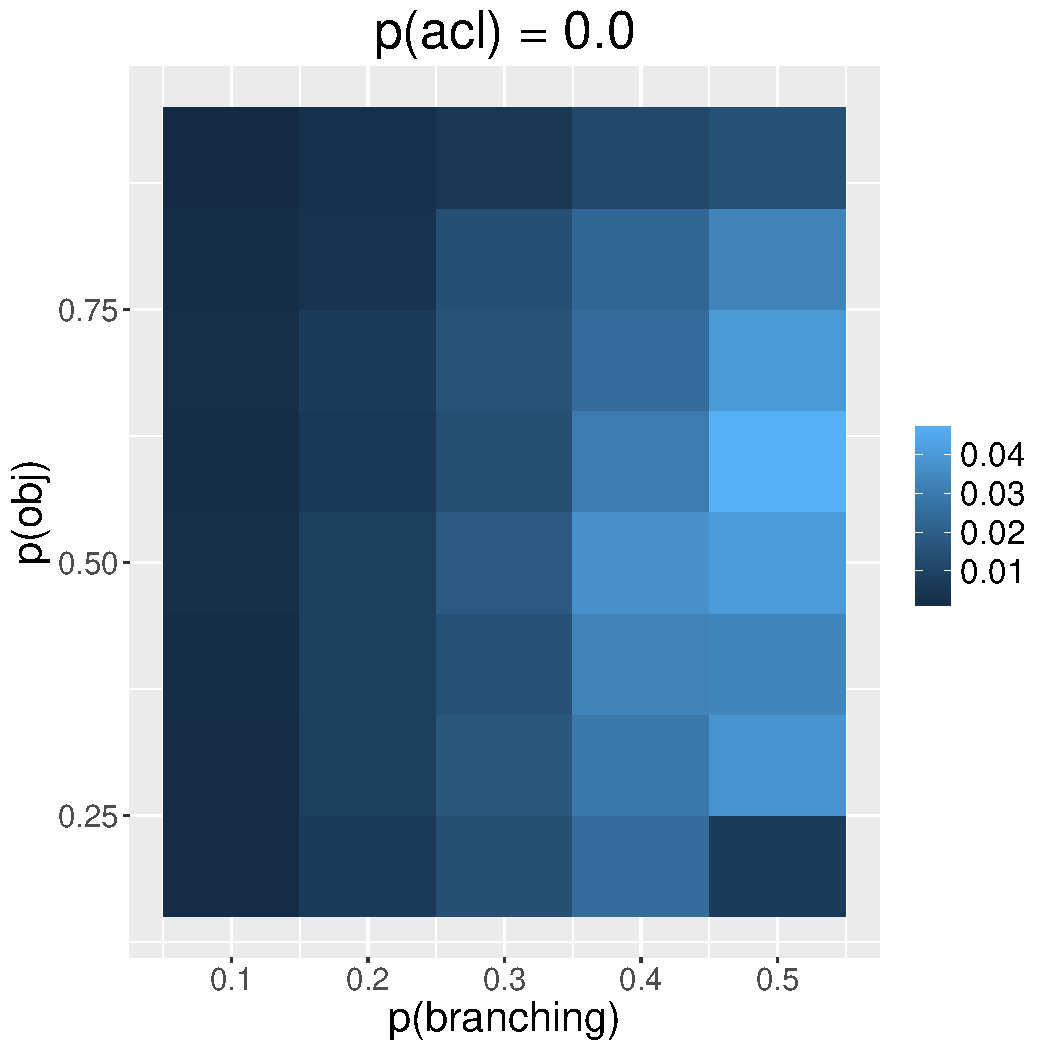
\includegraphics[width=0.4\textwidth]{../models/revision/toy_simulations/result_NPBranching0_0.pdf}
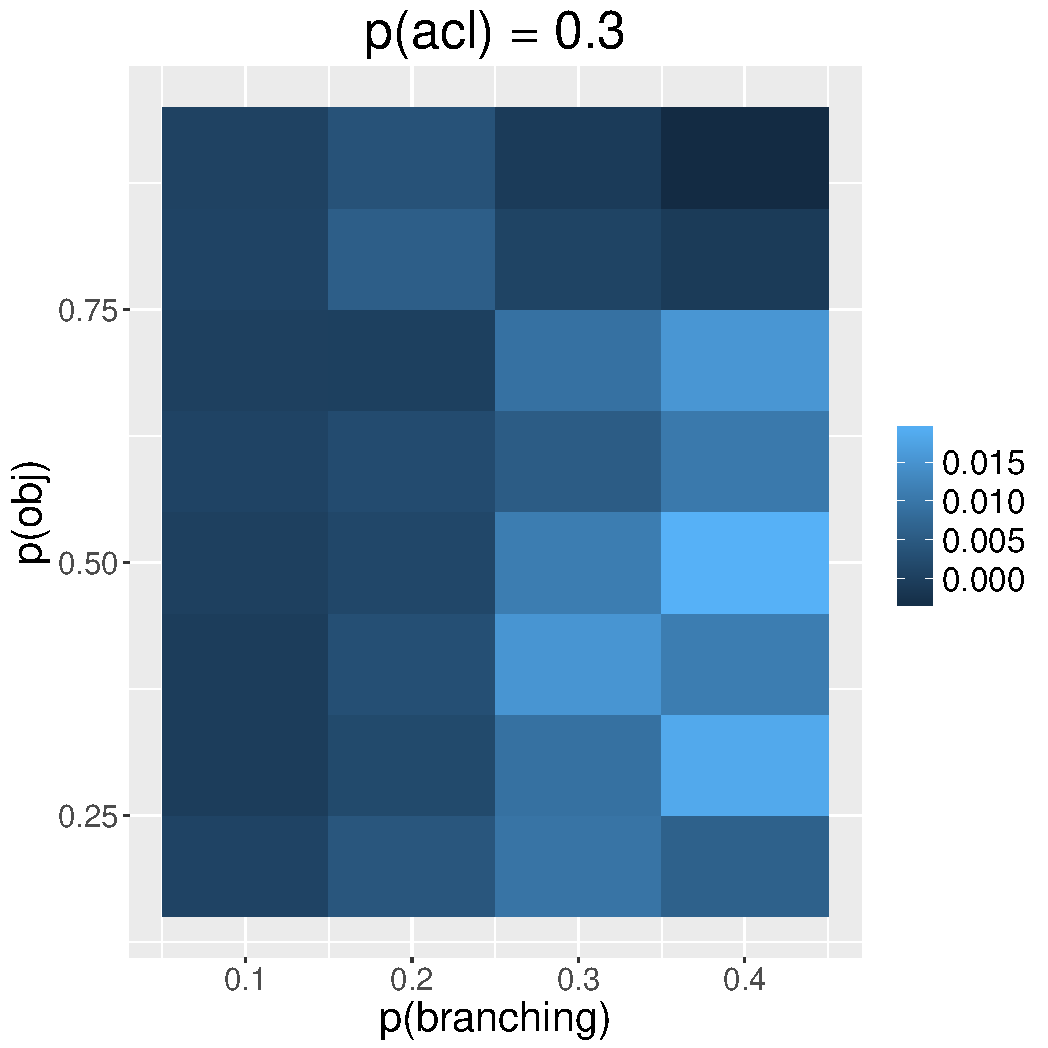
\includegraphics[width=0.4\textwidth]{../models/revision/toy_simulations/result_NPBranching0_3.pdf}
\end{center}

	\caption{Difference in parseability $I[\mathcal{T}, \mathcal{U}]$ (normalized by sentence length) between the correlating and anti-correlating grammars, for $p_\text{acl} = 0.0$ (left) and $p_\text{acl} = 0.3$ (right). Positive values indicate greater values of $I[\mathcal{T}, \mathcal{U}]$ for correlating grammars.}\label{fig:toy-parseability}
\end{figure}


Results are shown in Figure~\ref{fig:toy-parseability}. For almost all parameter regimes, the correlating grammars have better parseability than the anti-correlating grammars. This is especially the case for grammars with high $p_\text{branching}$. 

This simulation shows that correlations can in principle improve parseability in the controlled setting of such a model, without appeal to memory limitations; we leave a full graph-theoretical understanding to future work.


\nocite{diessel2001ordering, dryer1980positional, wals} 


\bibliographystyle{unsrtnat}
\bibliography{everything}


\end{document}



























%\paragraph{Analysis 2: Quantifying Degree of Pareto Optimality}
%
%TODO maybe we can scrap this part as it is harder to explain well, if Analysis 1 sufficient.
%
%
%\begin{figure}
%\centering
%	\begin{tabular}{llll}
%		(a) & (b) & (c) & (d) \\
%		\includegraphics[width=0.22\textwidth]{figures/isocline1.png}&
%		\includegraphics[width=0.22\textwidth]{figures/isocline2.png}&
%		\includegraphics[width=0.22\textwidth]{figures/isocline3.png}&
%\includegraphics[width=0.22\textwidth]{figures/isocline4.png}
%	\end{tabular}
%
%	\caption{Isolines: (a) The set of all possible baseline grammars forms a distribution in the parseability-predictability space.
%	The Pareto frontier consists of those points that are not dominated by any baseline grammar -- that is, those for which $P=0$: For points on this curve, no baseline grammar is both to their top and their right.
%	(b) Other grammars are dominated by some fractions $P > 0$ of baseline grammars. The two green crosses mark grammars that both are dominated by $P=0.05$ of baseline grammars. A blue curve connects all grammars dominated by exactly $P=0.05$ of baseline grammars.
%	(c) We observe a sample of $N=50$ baseline grammars, sampled uniformly from the set of baseline grammars. Samples will tend to concentrate in the high-density regions of the baseline distribution.
%	We also observe the efficiency of the real language (red cross) and an estimate of the Pareto frontier (blue line).
%	(d) We use the $50$ samples from the baseline grammar distribution to construct an estimate of the full abseline distibution, using the Dirichlet Process Gaussian Mixture Model. Using this inferred distribution, we estimate what fraction $P$ of baseline grammars dominate the real language, and the curve connecting all grammars dominated by the same fraction $P$ of baselines.
%	}\label{fig:isoline-explanation}
%\end{figure}
%
%
%\begin{figure}
%\centering
%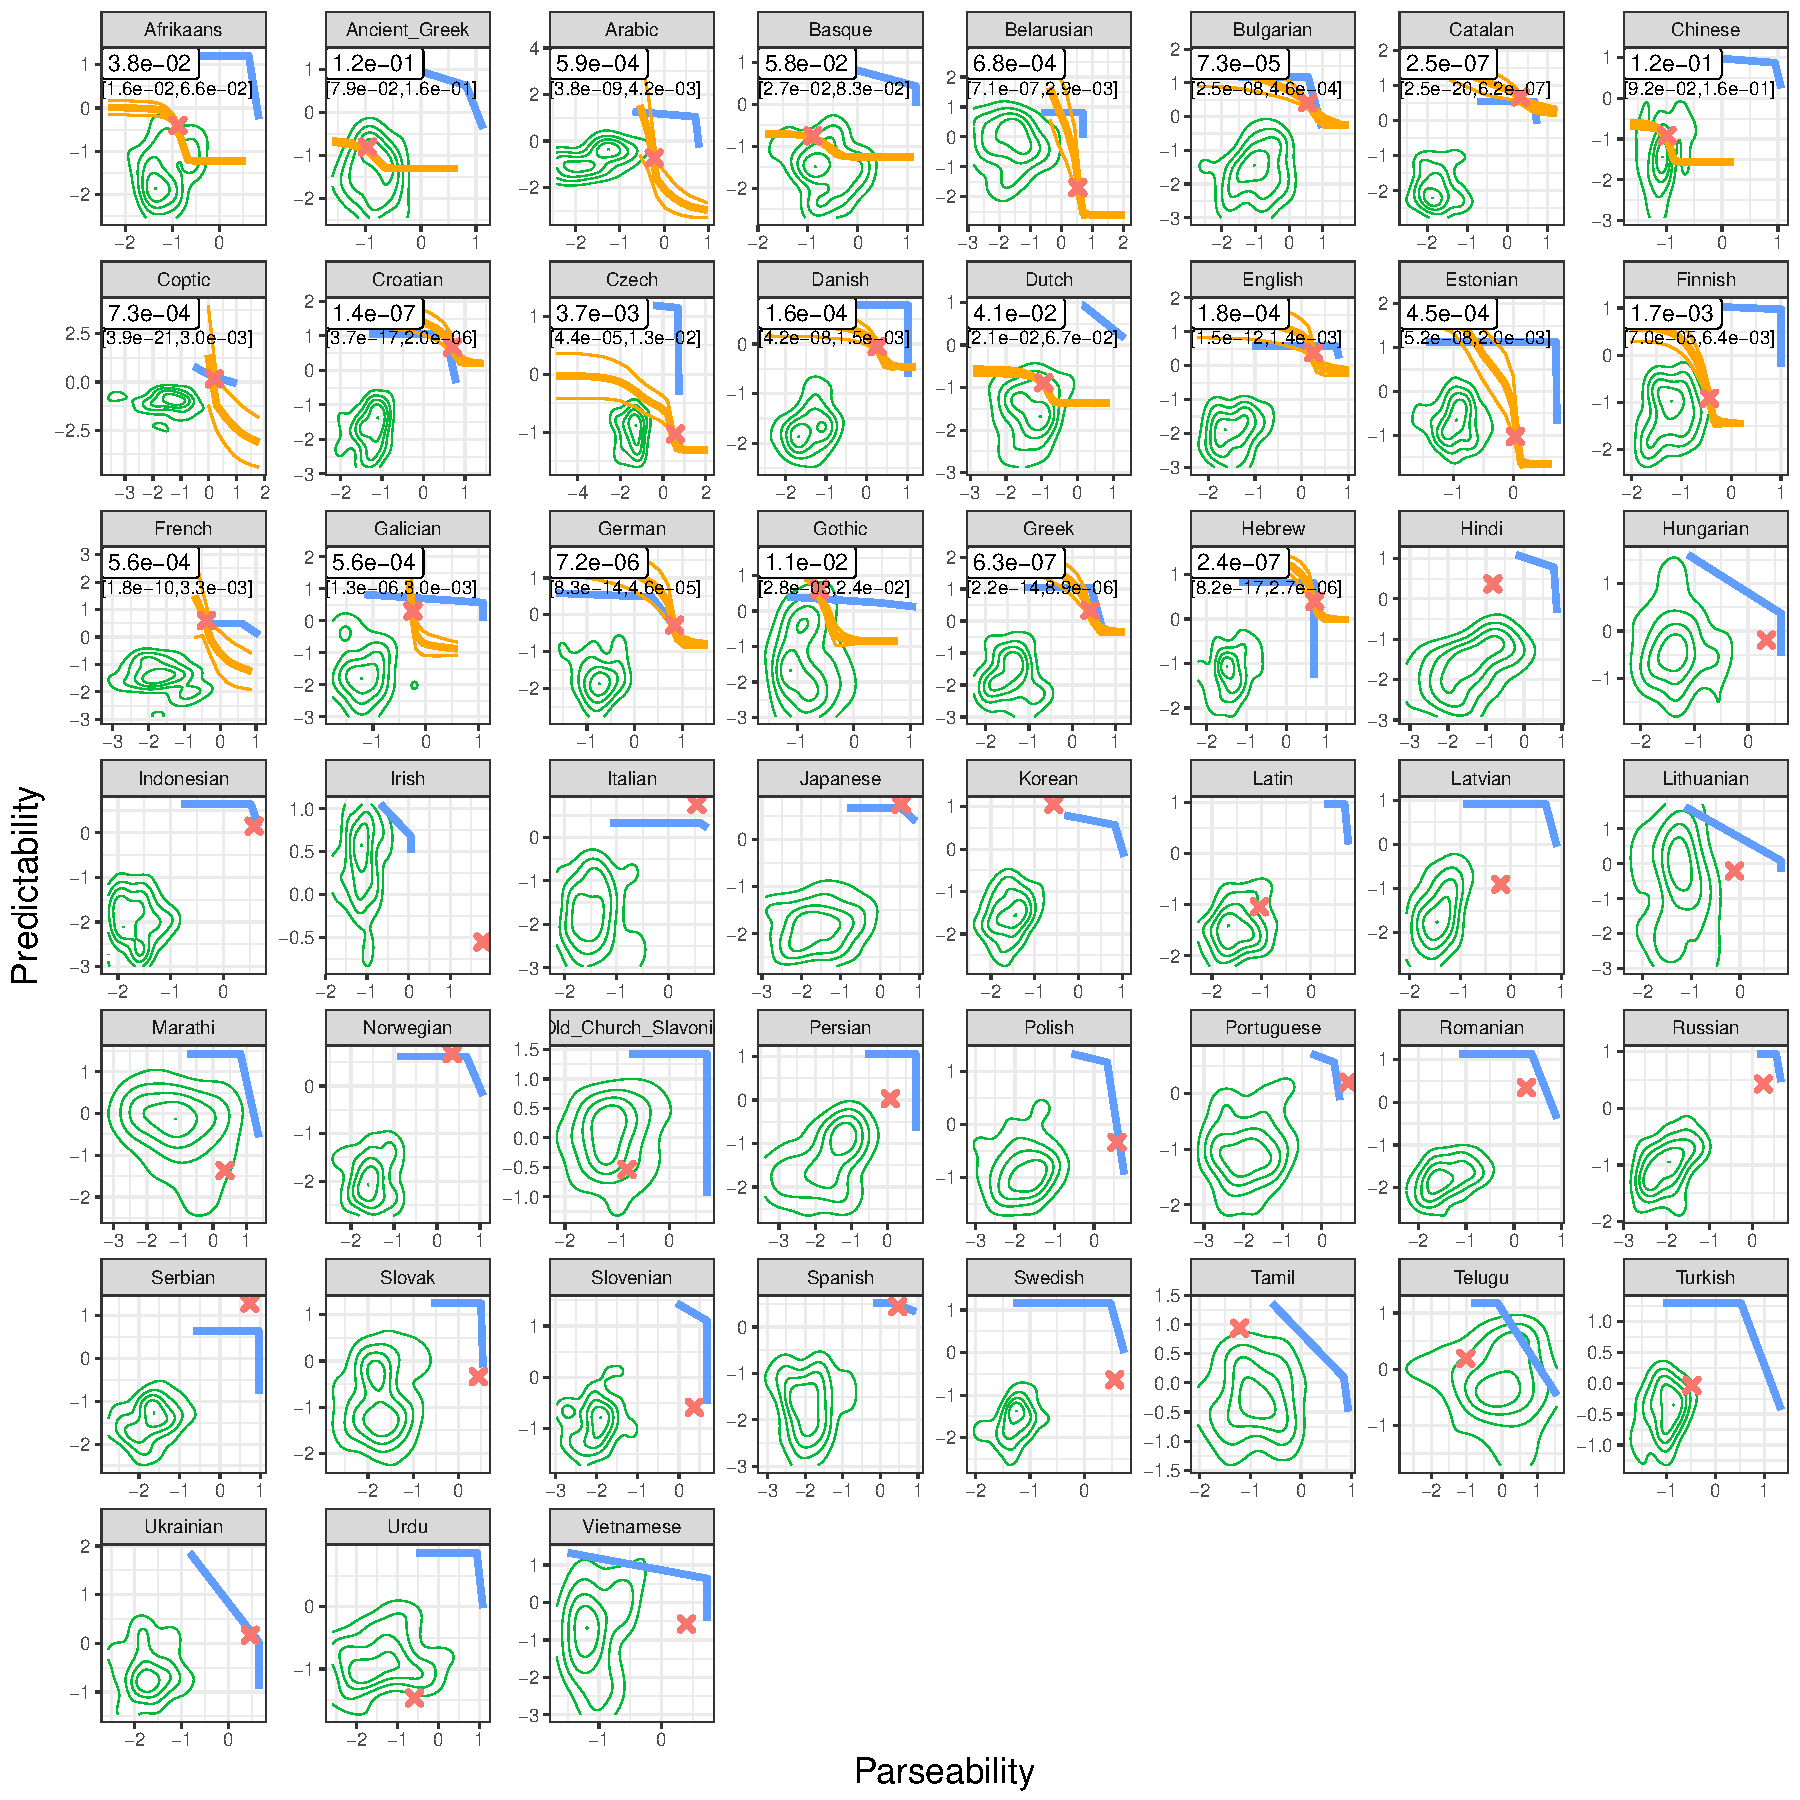
\includegraphics[width=\textwidth]{../results/plane/pareto-plane-perLanguage-isoCurve-smooth-interval.pdf}
%	\caption{Real languages, even those that are not at the estimated Pareto frontier, are Pareto-dominated by very few other hypothetical grammars. Green curves: Baseline distribution, estimated using Kernel Density estimation. Black numbers indicate the fraction of baselines dominating the real language, with a 95\% credible interval, estimated using a nonparametric Bayesian method (see text). Orange curves connect points estimated to be dominated by the same fraction of baselines as the real language, estimated using the same Bayesian method (see text). }\label{fig:isoline}
%\end{figure}
%
%
%%The Pareto curve is formed by those grammars such that no grammar simultaneously achieves higher parseability and higher predictability.
%%This motivates 
%
%We quantify the Pareto-optimality of the language $r$ as the fraction of baselines that Pareto-dominate $r$ -- that is, baselines that are at least as good as $r$ on \emph{both} parseability and predictability:
%\begin{equation}
%P := \frac{\# \{b \in B: R_{Pars}(b) \geq R_{eff}(r) \text{ and }  R_{Pred}(b) \geq R_{Pred}(r) \}}{\#B}
%\end{equation}
%%This quantifies how many hypothetical grammars are more efficient than $r$ for \emph{all} choices of $\lambda$ (make a figure).
%%This quantity is also known as the joint (or bivariate) exceedance probability.
%If we have access to the full distribution over baseline grammars, then the Pareto frontier is formed by exactly those grammars where $P=0$ (make a figure).
%(TODO slight subtlety: $r$ itself is part of $B$, so $P > 0$ TODO change definition)
%Small values of $P$ indicate that only few baseline grammars are better than $r$.
%%In practice, we only have a limited sample of $50$ baseline grammar samples; so only an approximation of $P$ is actually observable, and this approximation will be $0$ in a larger region of the plane (make a figure).
%
%In this section, we aim to estimate $P$, provide uncertainty intervals.
%In order to also compare with the values of $P$ attained by baseline languages, we also estimated the isoline (cotour line) of grammars having the same $P$ value as the real language.
%
%%$P$ is also known as the \emph{joint} or \emph{bivariate} \emph{exceedance probability}, and there are a range of methods for estimating it.
%
%We used a simple nonparametric Bayesian approach to estimate $P$ from the 50 observed baseline samples.
%The baseline languages form a distribution in the parseability-predictability plane, from which 50 independent samples are known.
%We model the underlying distribution using the Dirichlet Process Gaussian Mixture Model (DPGMM), a flexible nonparametric model that can accomodate multimodal and other non-normal distributions \citep{rasmussen2000infinite, escobar1995bayesian, muller1996bayesian}.
%This model is a Gaussian mixture model where the number of components itself is a latent parameter inferred from the data.
%DPGMMs can be seen as a Bayesian version of Kernel Density Smoothing.\footnote{A potential objection to using such Kernel Density Estimation is that it models a continuous distribution with support everywhere, while the distribution of grammars is discrete and finite, in particular bounded by a Pareto frontier. We believe that this does not cause problems for this analysis. First, the number of possible grammars is extremey large, exceeding $37!$, which is more than $10^{43}$, suggesting that the distribution in the parseability-predictability plane is closely approximated by a continuous distribution. Second, the approximate Pareto frontier tends to be clearly separated from the high-density regions of the baseline distribution, in which most sampled baselines fall, showing that the baseline distribution has very small density around and beyond the Pareto frontier.}
%In our context here, the reason for using DPGMMs instead of Kernel Density Smoothing is that Bayesian inference using the DPGMM provides a straightforward method of deriving estimates and credible intervals for $PO$ and the isoline.
%
%% http://mlg.eng.cam.ac.uk/pub/pdf/GoeRas10.pdf
%% TODO report prior
%
%The DPGMM defines a prior over possible baseline distributions in the parseability-predictability plane.
%%Under this prior, each possible distribution is parameterized by a number $n$ of components, $n$ bivariate Gaussians $\mu_i, \Sigma_i$, and $n$ weights $w_i$ for these components ($\sum_{i=1}^n w_i=1$).
%Each possible distribution is parameterized as $\sum_{i=1}^n w_i p_{\mu_i, \Sigma_i}(x)$ where $p_{\mu_i, \Sigma_i}$ is the bivariate Gaussian density.
%The number $n$ of components is inferred from the data together with the weights $w_i$, the means $\mu_i$, and the covariance matrices $\Sigma_i$.
%A Dirichlet process prior (TODO) is placed on $n$, favoring models with smaller numbers of components unless the data provides evidence for more components.
%We use the $50$ observed baseline samples to infer a posterior distribution over such mixture distributions.
%We then use MCMC to obtain 1,000 samples from the posterior, based on these samples.
%We used the MCMC implementation provided by the \texttt{R} \citep{R2013} package \texttt{dirichletprocess}~\citep{ross2018dirichletprocess}, discarding the first 1,000 samples as warmup samples, and obtaining another 1,000 samples, from which we selected an evenly spaced subset of 100 samples.
%
%For each of these samples, we then computed $P$ of the real language, and the isoline.
%The collection of these results provides a set of samples from the posterior distribution over the true value of $P$ and the true isoline.
%We plot the posterior means of $P$ and the isoline in Figure~\ref{fig:isoline}.
%
%
%
%
%




% paretoByFamily.R


%\paragraph{Inferring $\lambda$}
%We choose $\lambda$ to minimize the number of baselines that have better values of $R_\lambda := R_{Pars} + \lambda R_{Pred}$ than the real language:
%\begin{equation}
%	O := \min_\lambda \# \{b \in B: R_{eff}(b) > R_{eff}(r)\}
%\end{equation}
%where $r$ is the real language, and $B$ is the set of baselines.
%Naively choosing $\lambda$ to minimize this quantity from the observed $50$ baseline samples will bias $O$ towards overestimating the optimality of the real language.
%
%TODO maybe add a figure explaining the Bayesian story a bit more -- how we're using a continuous distribution to smooth out the observed samples?
%
%We eliminate this anti-conservative bias by conducting joint Bayesian inference of $\lambda$ of $O$, using the Dirichlet Gaussian Process, a Bayesian version of Kernel Density Smoothing.
%The 50 samples represent an underlying baseline distribution in the predictability-parseability plane.
%We approximate this underlying distribution as a continuous distribution from the Dirichlet Gaussian Process, and infer its parameters using Bayesian inference.
%We use this method to obtain a Bayesian estimate of the distribution of baseline distributions in the Surprisal-Parseability plane.
%The Dirichlet Gaussian Process (CITE) defines a prior over possible baseline distributions.
%Under this prior, each possible distribution is parameterized by a number $n$ of components, and $n$ Gaussians $\mu_n, \sigma^2_n$.
%Due to the flexible number of components, this nonparametric prior can accomodate a wide range of continuous probability distributions, including multimodal ones.
%We use the $50$ observed baseline samples to infer a posterior distribution over such smooth distributions.
%We then use MCMC to obtain 1,000 samples from the posterior, based on these samples.
%We used the MCMC implementation provided by the \texttt{R} \citep{R2013} package \texttt{dirichletprocess}~\citep{ross2018dirichletprocess}, discarding the first 1,000 samples as warmup samples, and obtaining another 1,000 samples.
%
%For every sampled distribution -- consisting of a component number $n$ and $n$ Gaussians, we then computed 
%\begin{equation}
%	O := \min_\lambda P(R_{eff}(b) > R_{eff}(r))\}
%\end{equation}
%where we considered $\lambda \in (0,1)$ in steps of $0.5$.
%
%By taking the values $O, \lambda$ for the 1,000 posterior samples, we obtained an estimate of the posterior of $O$ and $\lambda$.


